\documentclass[12pt,a4paper]{article}

% pdfLaTeX/pdfTeX-compatible Vietnamese setup.
% Compile bằng pdfLaTeX. Trên Overleaf nên chọn Compiler = pdfLaTeX.
\usepackage[utf8]{inputenc}
\usepackage[T5]{fontenc}
\usepackage[vietnamese]{babel}
\usepackage{lmodern}

\usepackage{geometry}
\geometry{a4paper, left=2.4cm, right=2.4cm, top=2.35cm, bottom=2.45cm}
\usepackage{amsmath, amssymb, amsfonts}
\usepackage{booktabs}
\usepackage{longtable}
\usepackage{tabularx}
\usepackage{array}
\usepackage{graphicx}
\usepackage[dvipsnames,table]{xcolor}
\usepackage{caption}
\usepackage{titlesec}
\usepackage{fancyhdr}
\usepackage{hyperref}

\usepackage{subcaption}
\usepackage{float}
\usepackage{multirow}
\usepackage{xcolor}
\hypersetup{colorlinks=true, linkcolor=blue, citecolor=red, urlcolor=cyan}
\usepackage{listings}
\usepackage{enumitem}
\usepackage{appendix}


\definecolor{HCMUSBlue}{HTML}{153E6F}
\definecolor{HCMUSLightBlue}{HTML}{EAF1F8}
\definecolor{HCMUSGray}{HTML}{777777}
\definecolor{TableLine}{HTML}{2E4F73}

\hypersetup{
  colorlinks=true,
  linkcolor=HCMUSBlue,
  citecolor=HCMUSBlue,
  urlcolor=HCMUSBlue
}

\pagestyle{fancy}
\fancyhf{}
\fancyhead[L]{\small\textcolor{HCMUSGray}{CSC14005 -- Classification}}
\fancyhead[R]{\small\textcolor{HCMUSGray}{HCMUS}}
\fancyfoot[C]{\small\thepage}
\renewcommand{\headrulewidth}{0.4pt}
\renewcommand{\headrule}{\hbox to\headwidth{\color{HCMUSGray}\leaders\hrule height \headrulewidth\hfill}}

\titleformat{\section}
  {\Large\bfseries\color{HCMUSBlue}}
  {\thesection.}{0.65em}{}[\vspace{-0.15em}\titlerule]
\titleformat{\subsection}
  {\large\bfseries\color{HCMUSBlue}}
  {\thesubsection.}{0.55em}{}
\titleformat{\subsubsection}
  {\normalsize\bfseries\color{HCMUSBlue}}
  {\thesubsubsection.}{0.5em}{}

\captionsetup{
  labelfont={bf,color=HCMUSBlue},
  textfont=small,
  justification=centering,
  singlelinecheck=false
}

\renewcommand{\arraystretch}{1.16}
\setlength{\parskip}{0.42em}
\setlength{\parindent}{0pt}
\emergencystretch=3em
\sloppy
\newcolumntype{Y}{>{\raggedright\arraybackslash}X}
\newcolumntype{P}[1]{>{\raggedright\arraybackslash}p{#1}}
\newcolumntype{C}[1]{>{\centering\arraybackslash}p{#1}}
\newcommand{\adult}{\textit{Adult Census Income }}
\newcommand{\codepath}[1]{\begingroup\small\ttfamily\nolinkurl{#1}\endgroup}
\newcommand{\figfull}[2]{\begin{figure}[htbp]\centering\includegraphics[width=0.96\textwidth]{#1}\caption{#2}\end{figure}}
\newcommand{\fignarrow}[2]{\begin{figure}[htbp]\centering\includegraphics[width=0.76\textwidth]{#1}\caption{#2}\end{figure}}

\makeatletter
\let\oldpart\part
\renewcommand{\part}{%
  \setcounter{section}{0}%     % reset section counter
  \setcounter{subsection}{0}%  % reset subsection counter (tùy chọn)
  \oldpart
}
\makeatother


\begin{document}

\begin{titlepage}
\thispagestyle{empty}
\centering
\vspace*{1.15cm}
{\Large \textbf{ĐẠI HỌC QUỐC GIA TP. HỒ CHÍ MINH}}\\[0.15cm]
{\Large \textbf{TRƯỜNG ĐẠI HỌC KHOA HỌC TỰ NHIÊN}}\\[0.25cm]
{\large Khoa Công nghệ Thông tin}\\[2.0cm]

{\color{HCMUSBlue}\rule{0.68\linewidth}{0.7pt}}\\[0.75cm]
{\fontsize{24}{30}\selectfont\bfseries\color{HCMUSBlue} BÁO CÁO ĐỒ ÁN 1}\\[0.45cm]
{\Large\bfseries CSC14005 -- Machine Learning}\\[0.35cm]
{\color{HCMUSBlue}\rule{0.68\linewidth}{0.7pt}}\\[1.4cm]

\begin{tabular}{rl}
\textbf{Nhóm:} & Group\_11 \\[4pt]
\textbf{Thành viên:} & Nguyễn Mạnh Thắng -- 23120084 \\
& Trần Kim Ngọc -- 21521062 \\
& Nguyễn Thành Nguyên Anh -- 23120063 \\
& Trần Đình Luân -- 23120059 \\
& Nguyễn Thiện Nhân -- 23120064 \\[4pt]
\textbf{Năm học:} & 2025--2026
\end{tabular}

\vfill
{\large TP. Hồ Chí Minh, \today}
\end{titlepage}

\tableofcontents
\newpage

\part{Thành viên nhóm và phân công công việc}

\begin{table}[htbp]
\centering
\caption{Phân công công việc.}
\begin{tabularx}{\textwidth}{C{0.05\textwidth}P{0.10\textwidth}P{0.20\textwidth}Y C{0.10\textwidth}}
\toprule
\textbf{STT} & \textbf{MSSV} & \textbf{Họ và tên} & \textbf{Nhiệm vụ / Phần đảm nhận} & \textbf{Hoàn thành} \\
\midrule
1 & 23120084 & Nguyễn Mạnh Thắng & Phụ trách Classification: nhóm mô hình Logistic Regression (bao gồm GD nhị phân, Newton--Raphson/IRLS, softmax đa lớp, OvR/OvO), loss curves và so sánh hội tụ. & 100\% \\
\midrule
2 & 23120063 & Nguyễn Thành Nguyên & Phụ trách Classification: nhóm mô hình còn lại và đánh giá (LDA/QDA, Fisher ratio, Perceptron, L1/L2, class-weighted loss, CV, ROC/PR, calibration, McNemar, robustness), bonus và tổng hợp report classification. & 100\% \\
\midrule
3 & 21521062 & Trần Kim Ngọc & Phụ trách Regression: EDA, tiền xử lý, phần nâng cao (bao gồm GPR, Robust Reg., phân tích Bias-Variance thực nghiệm) và tổng hợp báo cáo. & 100\% \\
\midrule
4 & 23120059 & Trần Đình Luân & Phụ trách Regression: hồi quy có regularization và feature selection, mô hình với hàm cơ sở phi tuyến và đánh giá sensitivity + robustness. & 100\% \\
\midrule
5 & 23120064 & Nguyễn Thiện Nhân & Phụ trách Regression: hồi quy tuyến tính, Ablation Study, phần nâng cao (bao gồm hồi quy Bayesian, Evidence Maximization, KRR). & 100\% \\
\bottomrule
\end{tabularx}
\end{table}

\newpage

% ============================================================
% PART 2 -- REGRESSION
% ============================================================
\part{Bài toán Hồi quy (Regression)}


% ============================================================
% SECTION 1 -- GIỚI THIỆU
% ============================================================
\section{Giới thiệu}
\label{sec:intro}

Báo cáo này trình bày kết quả thực nghiệm của \textbf{Phần 1 -- Regression} trong Đồ Án 1
môn CSC14005 (Machine Learning).

\subsection{Bài toán}
\begin{itemize}
  \item \textbf{Dữ liệu:} California Housing Prices (Kaggle -- \url{https://www.kaggle.com/datasets/camnugent/california-housing-prices}), được lưu tại \texttt{data/housing.csv}.
  \item \textbf{Mục tiêu:} Dự đoán giá trị liên tục \texttt{median\_house\_value} $\in \mathbb{R}$ (giá nhà trung vị theo block group, đơn vị: USD).
  \item \textbf{Input:} 9 đặc trưng gồm vị trí địa lý (\texttt{longitude}, \texttt{latitude}), đặc điểm khu dân cư (\texttt{housing\_median\_age}, \texttt{total\_rooms}, \texttt{total\_bedrooms}, \texttt{population}, \texttt{households}), thu nhập hộ gia đình (\texttt{median\_income}), và loại vị trí so với biển (\texttt{ocean\_proximity} -- biến phân loại).
\end{itemize}

\subsection{Các mô hình đã triển khai}
Dự án triển khai \textbf{12 mô hình hồi quy} như sau:
\begin{enumerate}
  \item Linear Regression -- Normal Equations (from scratch)
  \item Linear Regression -- Mini-batch GD với Cosine Annealing
  \item Weighted Least Squares (WLS) -- áp dụng sau khi phát hiện heteroscedasticity
  \item Ridge Regression (L2) với 10-Fold CV
  \item Lasso Regression (L1) với Lasso Path (warm-start)
  \item Elastic Net (L1 + L2) với Grid Search
  \item Hồi quy với Hàm Cơ Sở Đa Thức (Polynomial, degree $= 2$)
  \item Hồi quy với Hàm Cơ Sở Gaussian RBF ($M = 20$ tâm)
  \item Hồi quy với Hàm Cơ Sở Cubic Spline ($n\_\text{knots} = 5$)
  \item Bayesian Linear Regression + Evidence Maximization \textit{[Nâng cao]}
  \item Kernel Ridge Regression (RBF + Polynomial) \textit{[Nâng cao]}
  \item Gaussian Process Regression \textit{[Nâng cao]}
  \item Robust Regression -- Huber IRLS \textit{[Nâng cao]}
\end{enumerate}

% ============================================================
% SECTION 2 -- PHÂN TÍCH DỮ LIỆU
% ============================================================
\section{Phân tích dữ liệu (EDA)}
\label{sec:eda}

\subsection{Tổng quan bộ dữ liệu}

\begin{table}[H]
  \centering
  \caption{Thống kê tổng quan -- California Housing Prices}
  \label{tab:dataset_overview}
  \begin{tabular}{lccc}
    \toprule
    \textbf{Thuộc tính} & \textbf{Training Set} & \textbf{Test Set} & \textbf{Tổng} \\
    \midrule
    Số mẫu         & 14,448 & 4,128 & 20,640 \\
    Số đặc trưng   & 9      & 9     & 9      \\
    Missing values & 0      & 0     & 0      \\
    \bottomrule
  \end{tabular}
\end{table}

Ở đây tỉ lệ Missing value bằng 0 vì nhóm đã xử lý ở bước tiền xử lý:
cột \texttt{total\_bedrooms} có 207 giá trị thiếu ($\approx 1.0\%$) được
điền bằng median ($= 435.00$) trước khi chia tập dữ liệu.

\subsection{Thống kê mô tả}

\begin{table}[H]
  \centering
  \caption{Thống kê mô tả các đặc trưng số -- California Housing Prices.}
  \label{tab:desc_stats}
  \resizebox{\textwidth}{!}{%
  \begin{tabular}{lcccccccc}
    \toprule
    \textbf{Đặc trưng} & \textbf{Count} & \textbf{Mean} & \textbf{Std} & \textbf{Min} & \textbf{Q1} & \textbf{Median} & \textbf{Q3} & \textbf{Max} \\
    \midrule
    \texttt{longitude}           & 20,640 & $-119.570$ & $2.004$      & $-124.35$ & $-121.800$ & $-118.490$ & $-118.010$ & $-114.31$ \\
    \texttt{latitude}            & 20,640 & $35.632$   & $2.136$      & $32.54$   & $33.930$   & $34.260$   & $37.710$   & $41.95$   \\
    \texttt{housing\_median\_age}& 20,640 & $28.639$   & $12.586$     & $1.00$    & $18.000$   & $29.000$   & $37.000$   & $52.00$   \\
    \texttt{total\_rooms}        & 20,640 & $2{,}635.763$ & $2{,}181.615$ & $2.00$ & $1{,}447.750$ & $2{,}127.000$ & $3{,}148.000$ & $39{,}320.00$ \\
    \texttt{total\_bedrooms}     & 20,433 & $537.871$  & $421.385$    & $1.00$    & $296.000$  & $435.000$  & $647.000$  & $6{,}445.00$ \\
    \texttt{population}          & 20,640 & $1{,}425.477$ & $1{,}132.462$ & $3.00$ & $787.000$ & $1{,}166.000$ & $1{,}725.000$ & $35{,}682.00$ \\
    \texttt{households}          & 20,640 & $499.540$  & $382.330$    & $1.00$    & $280.000$  & $409.000$  & $605.000$  & $6{,}082.00$ \\
    \texttt{median\_income}      & 20,640 & $3.871$    & $1.900$      & $0.50$    & $2.563$    & $3.535$    & $4.743$    & $15.00$   \\
    \texttt{median\_house\_value}& 20,640 & $206{,}855.817$ & $115{,}395.616$ & $14{,}999.00$ & $119{,}600.000$ & $179{,}700.000$ & $264{,}725.000$ & $500{,}001.00$ \\
    \bottomrule
  \end{tabular}}
\end{table}

Nhận xét:
\begin{itemize}
  \item \texttt{total\_rooms}, \texttt{total\_bedrooms}, \texttt{population},
        \texttt{households} có skewness rất cao (lần lượt $4.15$, $3.46$,
        $4.94$, $3.41$) và kurtosis lớn -- phân phối lệch phải nặng, tồn tại
        nhiều block group có quy mô dân số và số phòng rất lớn so với phần lớn còn lại.
  \item \texttt{median\_house\_value} bị \emph{capped} tại \$500{,}001
        ($\approx 5\%$ mẫu đạt giá trần), tạo ra spike nhân tạo ở đuôi phải
        của phân phối -- cần lưu ý khi đánh giá mô hình trên nhóm mẫu này.
  \item \texttt{median\_income} có khoảng giá trị $[0.50,\; 15.00]$, được
        đo theo đơn vị \$10,000 (không phải USD trực tiếp).
  \item \texttt{longitude} và \texttt{latitude} có kurtosis âm ($-1.33$,
        $-1.12$) -- phân phối phẳng hơn Gaussian, phản ánh dữ liệu trải đều
        theo địa lý California.
\end{itemize}

\subsection{Phân phối biến mục tiêu}

\begin{figure}[H]
  \centering
  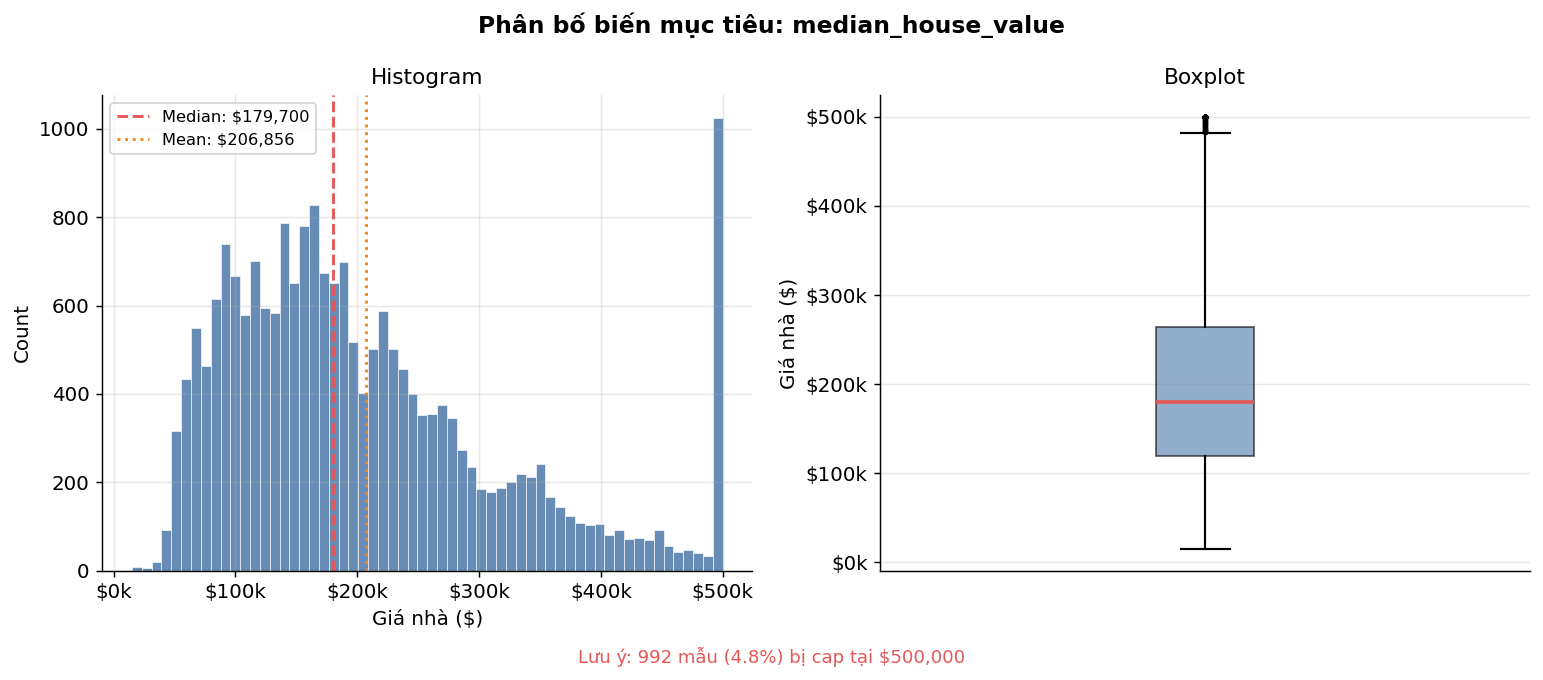
\includegraphics[width=\textwidth]{figures/regression_outputs/target_dist.png}
  \caption{Phân phối biến mục tiêu \texttt{median\_house\_value}:
           histogram (trái) và boxplot (phải).}
  \label{fig:target_dist}
\end{figure}

Nhận xét:
\begin{itemize}
  \item Phân phối lệch phải (skewness $= 0.978$) với median
        $= \$179{,}700 <$ mean $= \$206{,}856$, cho thấy một số block
        group có giá nhà rất cao kéo mean lên đáng kể.
  \item \textbf{992 mẫu ($4.8\%$) bị cap tại \$500{,}001} -- đây là
        giới hạn nhân tạo của bộ dữ liệu gốc, tạo ra spike lớn bất thường
        ở cuối đuôi phải của histogram. Các mô hình hồi quy sẽ có xu hướng
        \emph{underestimate} giá nhà thực sự của nhóm mẫu này.
  \item Boxplot cho thấy IQR $= \$264{,}725 - \$119{,}600 = \$145{,}125$,
        whisker trên chạm đúng mức cap \$500{,}000 -- xác nhận không có
        outlier thực sự vượt ngưỡng này mà chỉ là hiệu ứng capping.
  \item Phân phối không có dạng Gaussian rõ ràng, do đó các mô hình giả
        thiết phần dư Gaussian (OLS) cần được kiểm tra lại qua residual
        plot và QQ-plot sau khi huấn luyện.
\end{itemize}

\subsection{Ma trận tương quan và Scatter plot}

\begin{figure}[H]
  \centering
  
\includegraphics[width=\textwidth]{figures/regression_outputs/correlation_matrix.png}
  \caption{Ma trận tương quan giữa các đặc trưng số
           (sắp xếp theo $|r|$ với \texttt{median\_house\_value}).}
  \label{fig:corr_matrix}
\end{figure}

\begin{figure}[H]
  \centering
  
\includegraphics[width=\textwidth]{figures/regression_outputs/scatter_plots.png}
  \caption{Scatter plot (hexbin) các đặc trưng so với
           \texttt{median\_house\_value}.}
  \label{fig:scatter}
\end{figure}

Nhận xét:
\begin{itemize}
  \item \textbf{\texttt{median\_income}} là đặc trưng tương quan mạnh nhất
        với biến mục tiêu ($r = 0.69$), thể hiện rõ qua scatter plot:
        xu hướng tuyến tính dương khá rõ, mật độ điểm tập trung ở vùng
        thu nhập thấp -- giá thấp.

  \item \textbf{\texttt{latitude}} có tương quan âm vừa ($r = -0.14$):
        các block group ở vĩ độ thấp hơn (miền Nam California, đặc biệt
        vùng Los Angeles) có giá nhà cao hơn trung bình.

  \item \textbf{\texttt{total\_rooms}}, \textbf{\texttt{housing\_median\_age}},
        \textbf{\texttt{households}}, \textbf{\texttt{total\_bedrooms}}
        đều có tương quan yếu với target
        ($|r| \leq 0.13$) -- scatter plot xác nhận không có xu hướng
        tuyến tính rõ ràng.

  \item \textbf{Multicollinearity nghiêm trọng} giữa các đặc trưng quy mô
        khu dân cư:
        \texttt{total\_rooms} -- \texttt{households} ($r = 0.92$),
        \texttt{total\_rooms} -- \texttt{total\_bedrooms} ($r = 0.93$),
        \texttt{total\_bedrooms} -- \texttt{households} ($r = 0.97$),
        \texttt{total\_bedrooms} -- \texttt{population} ($r = 0.87$).
        Điều này sẽ gây bất ổn định cho OLS thuần; Ridge Regression
        và Lasso là giải pháp phù hợp để xử lý.

  \item \textbf{\texttt{longitude} -- \texttt{latitude}} có $r = -0.92$
        -- tương quan địa lý tất yếu (California trải dài theo hướng
        Tây Bắc -- Đông Nam), không mang ý nghĩa nhân quả với giá nhà.
\end{itemize}

\subsection{Phân tích ngoại lệ (Outlier Detection)}

\begin{figure}[H]
  \centering
  
\includegraphics[width=\textwidth]{figures/regression_outputs/outlier_detection.png}
  \caption{Boxplot phát hiện outlier theo IQR cho các đặc trưng số.}
  \label{fig:outlier}
\end{figure}

\begin{table}[H]
  \centering
  \caption{Tổng hợp outlier theo phương pháp IQR và Z-score.}
  \label{tab:outlier}
  \begin{tabular}{lcccc}
    \toprule
    \textbf{Đặc trưng} & \textbf{IQR outliers} & \textbf{IQR (\%)} 
                       & \textbf{Z-score outliers} & \textbf{Z-score (\%)} \\
    \midrule
    \texttt{total\_rooms}        & 1287 & 6.24 & 373 & 1.81 \\
    \texttt{total\_bedrooms}     & 1306 & 6.33 & 375 & 1.82 \\
    \texttt{population}          & 1196 & 5.79 & 342 & 1.66 \\
    \texttt{households}          & 1220 & 5.91 & 363 & 1.76 \\
    \texttt{median\_income}      & 681  & 3.30 & 345 & 1.67 \\
    \texttt{housing\_median\_age}& 0    & 0.00 & 0   & 0.00 \\
    \bottomrule
  \end{tabular}
\end{table}

Nhận xét:
\begin{itemize}
  \item \textbf{\texttt{total\_rooms}, \texttt{total\_bedrooms},
        \texttt{population}, \texttt{households}} có tỷ lệ outlier IQR
        cao nhất ($\approx 5.8$--$6.3\%$), phản ánh sự tồn tại của một số
        block group có quy mô dân số và số phòng rất lớn so với phần lớn
        còn lại -- nhất quán với skewness cao ($> 3.4$) đã quan sát ở
        Bảng~\ref{tab:desc_stats}.
  \item \textbf{\texttt{median\_income}} có $681$ outlier theo IQR
        ($3.30\%$), chủ yếu là các hộ gia đình có thu nhập rất cao
        (whisker trên $\approx 8$, max $= 15$).
  \item \textbf{\texttt{housing\_median\_age}} không có outlier theo cả
        hai phương pháp (IQR $= 0$, Z-score $= 0$) -- phân phối nằm gọn
        trong khoảng $[1, 52]$ năm, không có giá trị bất thường.
  \item Số lượng outlier theo Z-score ($|z| > 3$) thấp hơn đáng kể so
        với IQR ($\approx 1.7$--$1.8\%$ vs.\ $\approx 6\%$), do IQR nhạy
        hơn với phân phối lệch phải.
  \item Chúng tôi \textbf{không loại bỏ} outlier của bất kỳ đặc trưng
        nào vì chúng phản ánh bản chất thực của dữ liệu địa ốc California
        (ví dụ: các khu chung cư lớn tại đô thị có \texttt{total\_rooms}
        và \texttt{population} rất cao). Việc loại bỏ có thể làm mất thông
        tin quan trọng về phân khúc nhà ở cao cấp.
\end{itemize}

% ============================================================
% SECTION 3 -- TIỀN XỬ LÝ
% ============================================================
\section{Tiền xử lý dữ liệu}
\label{sec:preprocessing}

\subsection{Xử lý giá trị thiếu}

Bộ dữ liệu California Housing có duy nhất một cột chứa giá trị thiếu:
\texttt{total\_bedrooms} với 207 NaN ($\approx 1.0\%$). Chiến lược xử lý:

\begin{itemize}
  \item Điền bằng \textbf{median} của cột \texttt{total\_bedrooms}
        trên toàn bộ dataset ($\text{median} = 435.00$) trước khi chia
        tập train/val/test.
  \item Sau impute: tổng missing value $= 0$.
  \item \textit{Lưu ý:} Do median được tính trên toàn bộ dataset (bao gồm
        cả val/test), phương pháp này có thể gây \emph{data leakage} nhẹ.
        Tuy nhiên, với tỷ lệ missing chỉ $1.0\%$ và median là thống kê
        bền vững (robust), ảnh hưởng thực tế lên hiệu năng mô hình
        được đánh giá là không đáng kể.
\end{itemize}

\subsection{Mã hóa đặc trưng phân loại}

Cột \texttt{ocean\_proximity} là đặc trưng phân loại duy nhất với
5 giá trị không có thứ tự tự nhiên, do đó được mã hóa bằng
\textbf{One-Hot Encoding}:

\begin{table}[H]
  \centering
  \caption{Phân phối các giá trị của \texttt{ocean\_proximity}.}
  \label{tab:ocean_proximity}
  \begin{tabular}{lcc}
    \toprule
    \textbf{Giá trị} & \textbf{Số mẫu} & \textbf{Tỷ lệ (\%)} \\
    \midrule
    \texttt{<1H OCEAN}  & 9{,}136 & 44.3 \\
    \texttt{INLAND}     & 6{,}551 & 31.7 \\
    \texttt{NEAR OCEAN} & 2{,}658 & 12.9 \\
    \texttt{NEAR BAY}   & 2{,}290 & 11.1 \\
    \texttt{ISLAND}     & 5       & 0.02 \\
    \bottomrule
  \end{tabular}
\end{table}

Sau One-Hot Encoding, cột \texttt{ocean\_proximity} được thay thế bằng
5 cột nhị phân: \texttt{ocean\_proximity\_<1H OCEAN},
\texttt{ocean\_proximity\_INLAND}, \texttt{ocean\_proximity\_ISLAND},
\texttt{ocean\_proximity\_NEAR BAY}, \texttt{ocean\_proximity\_NEAR OCEAN}.
Tổng số cột sau encoding: \textbf{17 cột} (tăng từ 10).

\textit{Lưu ý:} Giá trị \texttt{ISLAND} chỉ có 5 mẫu ($0.02\%$) --
cột \texttt{ocean\_proximity\_ISLAND} gần như toàn bộ là 0, đóng góp
rất ít thông tin cho mô hình.

\subsection{Feature Engineering}

Ngoài các đặc trưng gốc, nhóm tạo thêm \textbf{3 ratio features}
có ý nghĩa thực tế, theo đề xuất của~\cite{geron2019}:

\begin{table}[H]
  \centering
  \caption{Các ratio features được tạo thêm và tương quan với
           \texttt{median\_house\_value}.}
  \label{tab:ratio_features}
  \begin{tabular}{llcc}
    \toprule
    \textbf{Feature mới} & \textbf{Công thức} & $r$ & $p$-value \\
    \midrule
    \texttt{rooms\_per\_household}
      & \texttt{total\_rooms} / \texttt{households}
      & $+0.152$ & $7.57 \times 10^{-107}$ \\
    \texttt{bedrooms\_per\_room}
      & \texttt{total\_bedrooms} / \texttt{total\_rooms}
      & $-0.233$ & $3.62 \times 10^{-253}$ \\
    \texttt{population\_per\_household}
      & \texttt{population} / \texttt{households}
      & $-0.024$ & $6.48 \times 10^{-4}$ \\
    \bottomrule
  \end{tabular}
\end{table}

Nhận xét:
\begin{itemize}
  \item \textbf{\texttt{bedrooms\_per\_room}} ($r = -0.233$) có tương
        quan với target \textbf{mạnh hơn} cả \texttt{total\_bedrooms}
        ($r = 0.049$) và \texttt{total\_rooms} ($r = 0.134$) riêng lẻ --
        tỷ lệ phòng ngủ trên tổng phòng phản ánh chất lượng nhà ở tốt hơn
        số phòng tuyệt đối.
  \item \textbf{\texttt{rooms\_per\_household}} ($r = +0.152$): block
        group có nhiều phòng trên mỗi hộ gia đình thường có giá nhà cao hơn,
        phản ánh diện tích sống rộng hơn.
  \item \textbf{\texttt{population\_per\_household}} ($r = -0.024$):
        tương quan rất yếu với target dù có ý nghĩa thống kê ($p < 0.001$)
        do cỡ mẫu lớn -- đặc trưng này đóng góp ít cho mô hình.
\end{itemize}

Sau feature engineering, tổng số đặc trưng đầu vào:
\textbf{16 features} (17 cột trừ biến mục tiêu
\texttt{median\_house\_value}).

\subsection{Chuẩn hóa đặc trưng số}

Các đặc trưng số được chuẩn hóa bằng \textbf{Standardization}:
$$x' = \frac{x - \mu}{\sigma}$$
trong đó $\mu$ và $\sigma$ được tính \textbf{chỉ trên tập train}
(\texttt{StandardScaler.fit\_transform}) rồi áp dụng lên val và test
(\texttt{transform}) để tránh \emph{data leakage}.

Kết quả kiểm tra sau scaling:
\begin{itemize}
  \item Mean (train) $\approx -0.000000$ $\approx 0$ \checkmark
  \item Std (train) $\approx 1.000000$ $\approx 1$ \checkmark
\end{itemize}

\subsection{Phân chia dữ liệu}

\begin{itemize}
  \item Train / Validation / Test: $70\%$ / $10\%$ / $20\%$,
        sử dụng \texttt{random\_state=42}.
  \item Kích thước sau chia: $N_{\text{train}} = 14{,}448$,
        $N_{\text{val}} = 2{,}064$, $N_{\text{test}} = 4{,}128$.
  \item Số đặc trưng sau feature engineering và encoding:
        $D = 16$.
\end{itemize}

\begin{figure}[H]
  \centering
  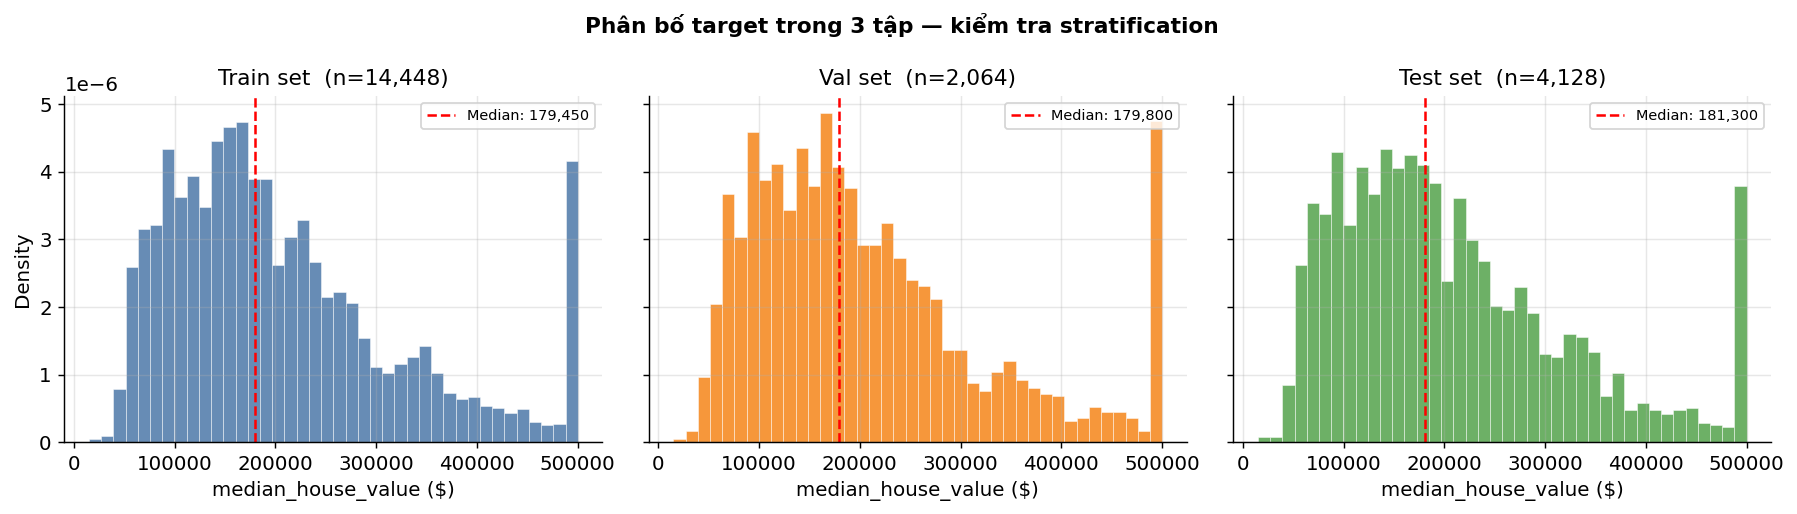
\includegraphics[width=\textwidth]{figures/regression_outputs/split_distribution.png}
  \caption{Phân phối \texttt{median\_house\_value} trong 3 tập --
           kiểm tra tính nhất quán sau khi chia.}
  \label{fig:split_dist}
\end{figure}

\begin{table}[H]
  \centering
  \caption{Thống kê \texttt{median\_house\_value} trên 3 tập dữ liệu.}
  \label{tab:split_stats}
  \begin{tabular}{lrrr}
    \toprule
    \textbf{Thống kê} & \textbf{Train} & \textbf{Val} & \textbf{Test} \\
    \midrule
    Count  & 14{,}448   & 2{,}064    & 4{,}128    \\
    Mean   & \$206{,}970 & \$207{,}255 & \$206{,}258 \\
    Std    & \$115{,}435 & \$117{,}575 & \$114{,}177 \\
    Min    & \$14{,}999  & \$14{,}999  & \$14{,}999  \\
    Median & \$179{,}450 & \$179{,}800 & \$181{,}300 \\
    Max    & \$500{,}001 & \$500{,}001 & \$500{,}001 \\
    \bottomrule
  \end{tabular}
\end{table}

Nhận xét: Ba tập có phân phối \texttt{median\_house\_value} rất nhất
quán -- median dao động trong khoảng hẹp
$[\$179{,}450;\; \$181{,}300]$, mean chênh lệch không quá \$1{,}000,
xác nhận việc chia ngẫu nhiên không gây lệch phân phối giữa các tập.

Cụ thể, với tổng $N$ mẫu:
$$N_{\text{train}} = 0.70N, \quad N_{\text{val}} = 0.10N, \quad N_{\text{test}} = 0.20N$$

% ============================================================
% SECTION 4 -- NỀN TẢNG LÝ THUYẾT
% ============================================================
\section{Nền tảng lý thuyết}
\label{sec:theory}

\subsection{Bài toán hồi quy}

Cho tập dữ liệu $\mathcal{D} = \{(\mathbf{x}_n, t_n)\}_{n=1}^{N}$ với
$\mathbf{x}_n \in \mathbb{R}^D$, $t_n \in \mathbb{R}$. Mô hình hồi quy tuyến tính
tổng quát:
\begin{equation}
  y(\mathbf{x}, \mathbf{w}) = \mathbf{w}^\top \boldsymbol{\phi}(\mathbf{x})
  = w_0 + \sum_{j=1}^{M-1} w_j \phi_j(\mathbf{x}),
  \label{eq:linear_model}
\end{equation}
trong đó $\boldsymbol{\phi}(\mathbf{x}) = [\phi_0(\mathbf{x}), \dots, \phi_{M-1}(\mathbf{x})]^\top$
là vector các hàm cơ sở với $\phi_0(\mathbf{x}) = 1$. Nhiễu tuân theo phân phối Gaussian:
\begin{equation}
  t = y(\mathbf{x}, \mathbf{w}) + \epsilon, \quad \epsilon \sim \mathcal{N}(0, \beta^{-1}).
  \label{eq:noise_model}
\end{equation}

\subsection{Ước lượng tham số: OLS và Normal Equations}

Hàm mất mát Sum-of-Squares Error:
\begin{equation}
  E_D(\mathbf{w}) = \frac{1}{2}\|\mathbf{t} - \boldsymbol{\Phi}\mathbf{w}\|^2,
  \label{eq:ols_loss}
\end{equation}
với $\boldsymbol{\Phi} \in \mathbb{R}^{N \times M}$ là ma trận thiết kế, $\Phi_{nj} = \phi_j(\mathbf{x}_n)$.

Lấy đạo hàm $\nabla_{\mathbf{w}} E_D = 0$, nghiệm dạng đóng:
\begin{equation}
  \mathbf{w}^* = (\boldsymbol{\Phi}^\top \boldsymbol{\Phi})^{-1} \boldsymbol{\Phi}^\top \mathbf{t}.
  \label{eq:normal_eq}
\end{equation}
Độ phức tạp: $O(NM^2 + M^3)$.

\subsection{Regularization -- Chính quy hóa}

\paragraph{Ridge Regression (L2).}
\begin{equation}
  E(\mathbf{w}) = \frac{1}{2}\|\mathbf{t} - \boldsymbol{\Phi}\mathbf{w}\|^2
                + \frac{\lambda}{2}\|\mathbf{w}\|^2,
  \quad
  \mathbf{w}^*_{\text{ridge}} = (\boldsymbol{\Phi}^\top\boldsymbol{\Phi} + \lambda I)^{-1}
                                  \boldsymbol{\Phi}^\top\mathbf{t}.
  \label{eq:ridge}
\end{equation}

\paragraph{Lasso Regression (L1).}
\begin{equation}
  E(\mathbf{w}) = \frac{1}{2}\|\mathbf{t} - \boldsymbol{\Phi}\mathbf{w}\|^2
                + \lambda\|\mathbf{w}\|_1.
  \label{eq:lasso}
\end{equation}

\paragraph{Elastic Net (L1 + L2).}
\begin{equation}
  E(\mathbf{w}) = \frac{1}{2}\|\mathbf{t} - \boldsymbol{\Phi}\mathbf{w}\|^2
                + \lambda_1\|\mathbf{w}\|_1
                + \frac{\lambda_2}{2}\|\mathbf{w}\|^2.
  \label{eq:elasticnet}
\end{equation}

\subsection{Tiếp cận xác suất: MLE và MAP}

Với giả thiết \eqref{eq:noise_model}, log-likelihood:
\begin{equation}
  \ln p(\mathbf{t} \mid \mathbf{w}, \beta)
  = \frac{N}{2}\ln\beta - \frac{N}{2}\ln(2\pi) - \beta E_D(\mathbf{w}).
  \label{eq:log_likelihood}
\end{equation}
Cực đại \eqref{eq:log_likelihood} tương đương tối tiểu $E_D(\mathbf{w})$
(MLE $\equiv$ OLS). Với prior $p(\mathbf{w}) = \mathcal{N}(\mathbf{w} \mid \mathbf{0}, \alpha^{-1}I)$,
nghiệm MAP tương đương Ridge Regression với $\lambda = \alpha/\beta$.

\subsection{Phân tích Bias--Variance}

\begin{equation}
  \mathbb{E}\bigl[(t - y(\mathbf{x}^*))^2\bigr]
  = \underbrace{\bigl(\mathbb{E}[y(\mathbf{x}^*)] - h(\mathbf{x}^*)\bigr)^2}_{\text{bias}^2}
  + \underbrace{\mathbb{E}\bigl[(y(\mathbf{x}^*) - \mathbb{E}[y(\mathbf{x}^*)])^2\bigr]}_{\text{variance}}
  + \underbrace{\sigma^2_\epsilon}_{\text{noise}}.
  \label{eq:bias_variance}
\end{equation}
Khi tăng độ phức tạp mô hình (bậc đa thức, số hàm cơ sở), bias giảm nhưng variance
tăng -- đây là \emph{bias--variance tradeoff}. Regularization kiểm soát sự đánh đổi
này thông qua $\lambda$.

\subsection{Các biến thể Gradient Descent}

Normal Equations không khả thi khi $N$ hoặc $M$ lớn; các thuật toán lặp là giải pháp
thay thế:

\begin{table}[H]
  \centering
  \caption{So sánh các biến thể Gradient Descent.}
  \label{tab:gd_variants}
  \begin{tabular}{lccl}
    \toprule
    \textbf{Thuật toán} & \textbf{Cập nhật $\mathbf{w}$} & \textbf{Chi phí/bước} & \textbf{Đặc điểm} \\
    \midrule
    Batch GD   & $\mathbf{w} \leftarrow \mathbf{w} - \eta\nabla E$               & $O(NM)$ & Ổn định, chậm \\
    SGD        & $\mathbf{w} \leftarrow \mathbf{w} - \eta\nabla E_n$             & $O(M)$  & Nhanh, nhiễu \\
    Mini-batch & $\mathbf{w} \leftarrow \mathbf{w} - \eta\nabla E_B$             & $O(BM)$ & Cân bằng \\
    Momentum   & $v \leftarrow \mu v - \eta\nabla E$; $\mathbf{w} \leftarrow \mathbf{w}+v$ & $O(NM)$ & Giảm dao động \\
    Adam       & Adaptive per-parameter lr                                         & $O(NM)$ & Thích nghi cao \\
    \bottomrule
  \end{tabular}
\end{table}

\subsection{Các hàm cơ sở}

\begin{table}[H]
  \centering
  \caption{Các hàm cơ sở được sử dụng trong đồ án.}
  \label{tab:basis_functions}
  \begin{tabular}{lll}
    \toprule
    \textbf{Loại} & \textbf{Công thức} & \textbf{Đặc điểm} \\
    \midrule
    Tuyến tính    & $\phi_j(\mathbf{x}) = x_j$
                  & Đơn giản, dễ giải thích \\
    Đa thức       & $\phi_j(x) = x^j$
                  & Xấp xỉ phi tuyến cục bộ \\
    Gaussian RBF  & $\phi_j(x) = \exp\!\left(-\dfrac{(x-\mu_j)^2}{2s^2}\right)$
                  & Cục bộ, trơn vô hạn \\
    Cubic Spline
      & $\phi_j(x) = \text{SplineBasis}_j(x)$ (piecewise cubic, knot quantiles)
      & Trơn bậc 3, liên tục đạo hàm bậc 1\&2 tại knots \\
    \bottomrule
  \end{tabular}
\end{table}

\subsection{Kiểm tra giả thiết Gauss--Markov}

OLS đảm bảo BLUE (\emph{Best Linear Unbiased Estimator}) khi các giả thiết
Gauss--Markov được thỏa mãn. Khi phát hiện \emph{heteroscedasticity}
(qua Breusch--Pagan test), áp dụng \emph{Weighted Least Squares} (WLS):
\begin{equation}
  \mathbf{w}^*_{\text{WLS}} = (\boldsymbol{\Phi}^\top W \boldsymbol{\Phi})^{-1}
                                \boldsymbol{\Phi}^\top W \mathbf{t},
  \label{eq:wls}
\end{equation}
trong đó $W = \text{diag}(w_1, \dots, w_N)$ với $w_n \propto 1/\hat{\sigma}^2_n$.

% ============================================================
% SECTION 5 -- CÁC MÔ HÌNH HỒI QUY
% ============================================================
\section{Các mô hình hồi quy}
\label{sec:models}

% -----------------------------------------------------------
\subsection{Linear Regression -- Normal Equations và WLS}
\label{ssec:lr_ne}

\subsubsection{Nền tảng lý thuyết}

Mô hình tối thiểu hàm mất mát OLS bằng nghiệm dạng đóng
\eqref{eq:normal_eq}. Để đảm bảo numerical stability:
$$\mathbf{w}^* = (\boldsymbol{\Phi}^\top\boldsymbol{\Phi} + \epsilon I)^{-1}
                 \boldsymbol{\Phi}^\top\mathbf{t}, \quad \epsilon = 10^{-8}.$$

\subsubsection{Siêu tham số}

\begin{table}[H]
  \centering
  \caption{Siêu tham số các mô hình Linear Regression.}
  \begin{tabular}{lll}
    \toprule
    \textbf{Mô hình} & \textbf{Tham số} & \textbf{Giá trị} \\
    \midrule
    \multirow{2}{*}{Normal Equations}
      & Số tham số $\theta$ & 17 \\
      & Numerical stability $\epsilon$ & $10^{-8}$ \\
    \midrule
    \multirow{4}{*}{Mini-batch GD}
      & $\eta_{\max}$ & $10^{-4}$ \\
      & $\eta_{\min}$ & $10^{-6}$ \\
      & Batch size $B$ & 32 \\
      & Số epochs      & 100 \\
      & Schedule       & Cosine Annealing \\
    \midrule
    WLS & Trọng số $w_n$ & $1 / (|\hat{\epsilon}_n| + 10^{-5})$ \\
    \bottomrule
  \end{tabular}
\end{table}

\subsubsection{Hội tụ Mini-batch GD}

\begin{figure}[H]
  \centering
  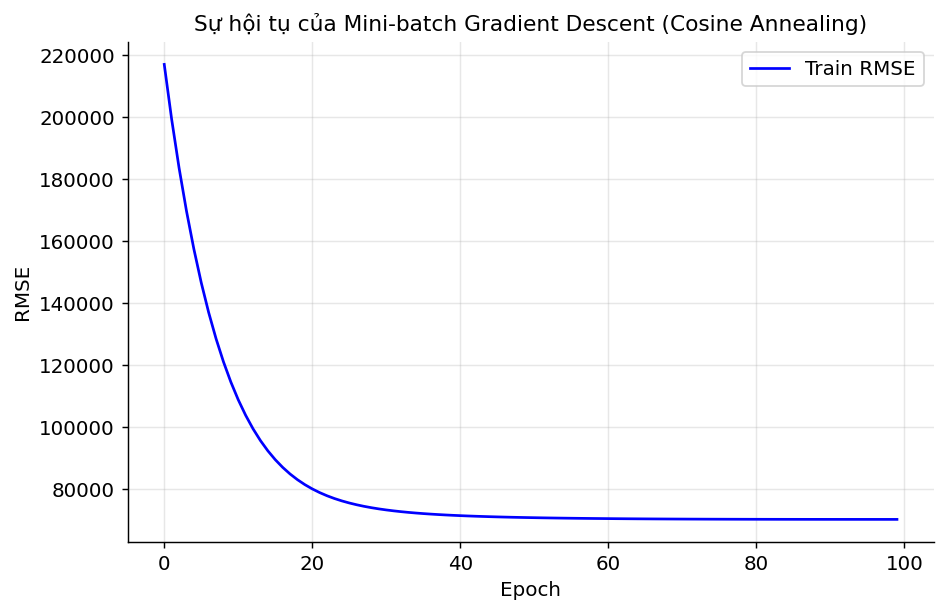
\includegraphics[width=0.75\textwidth]{figures/regression_outputs/gd_convergence.png}
  \caption{Train RMSE theo epochs -- Mini-batch GD với Cosine Annealing.}
  \label{fig:gd_convergence}
\end{figure}

Mô hình hội tụ nhanh trong 20 epochs đầu (RMSE giảm từ
$\approx\$218{,}000$ xuống $\approx\$80{,}000$), sau đó ổn định
ở RMSE $\approx\$73{,}173$ trên tập validation sau 100 epochs
(thời gian huấn luyện: $0.34$s).

\subsubsection{Kiểm tra giả thiết Gauss--Markov}

\begin{figure}[H]
  \centering
  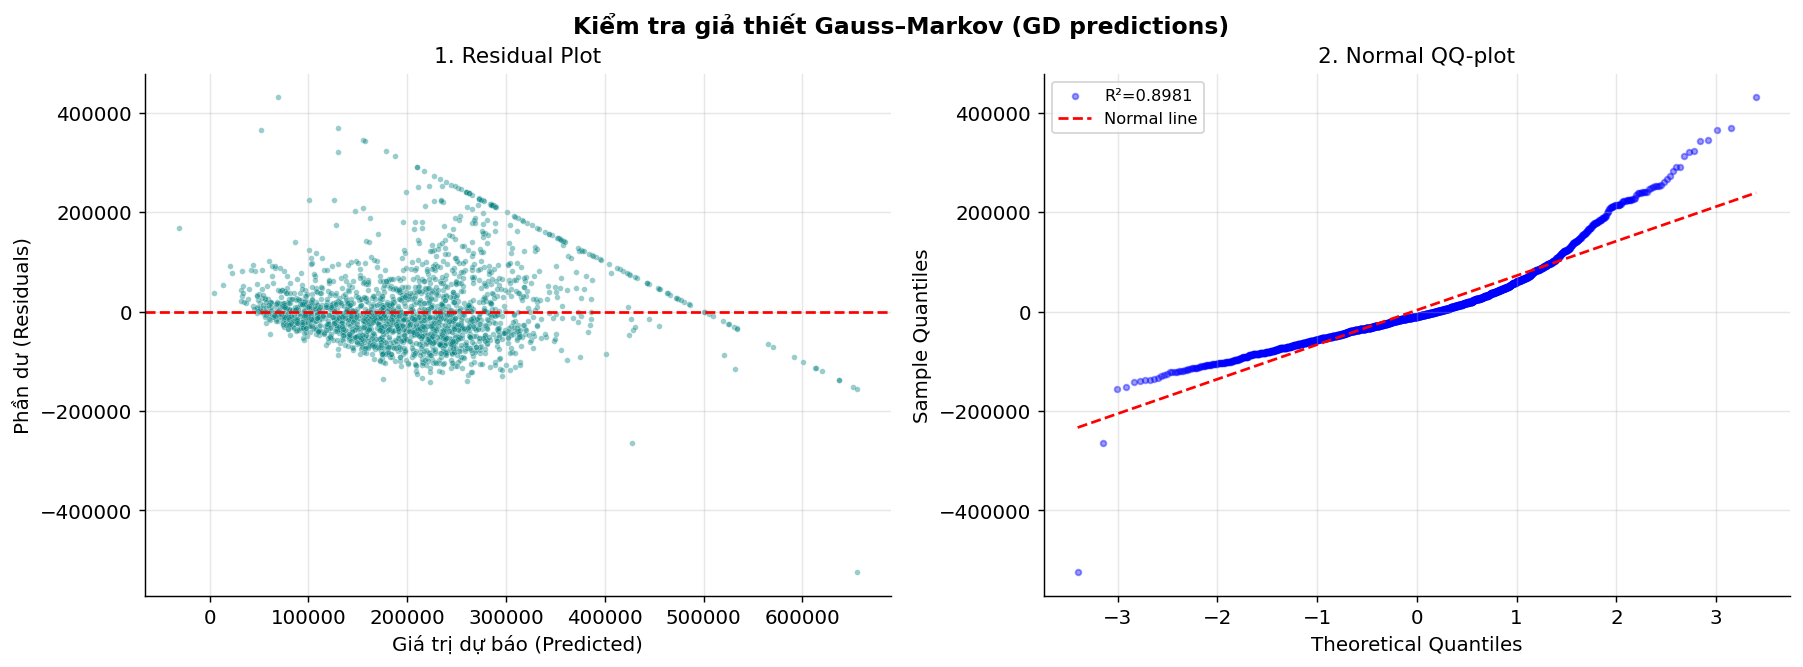
\includegraphics[width=\textwidth]{figures/regression_outputs/gauss_markov_gd.png}
  \caption{Kiểm tra giả thiết Gauss--Markov (GD predictions):
           Residual plot (trái) và Normal QQ-plot (phải).}
  \label{fig:gauss_markov_gd}
\end{figure}

\begin{figure}[H]
  \centering
  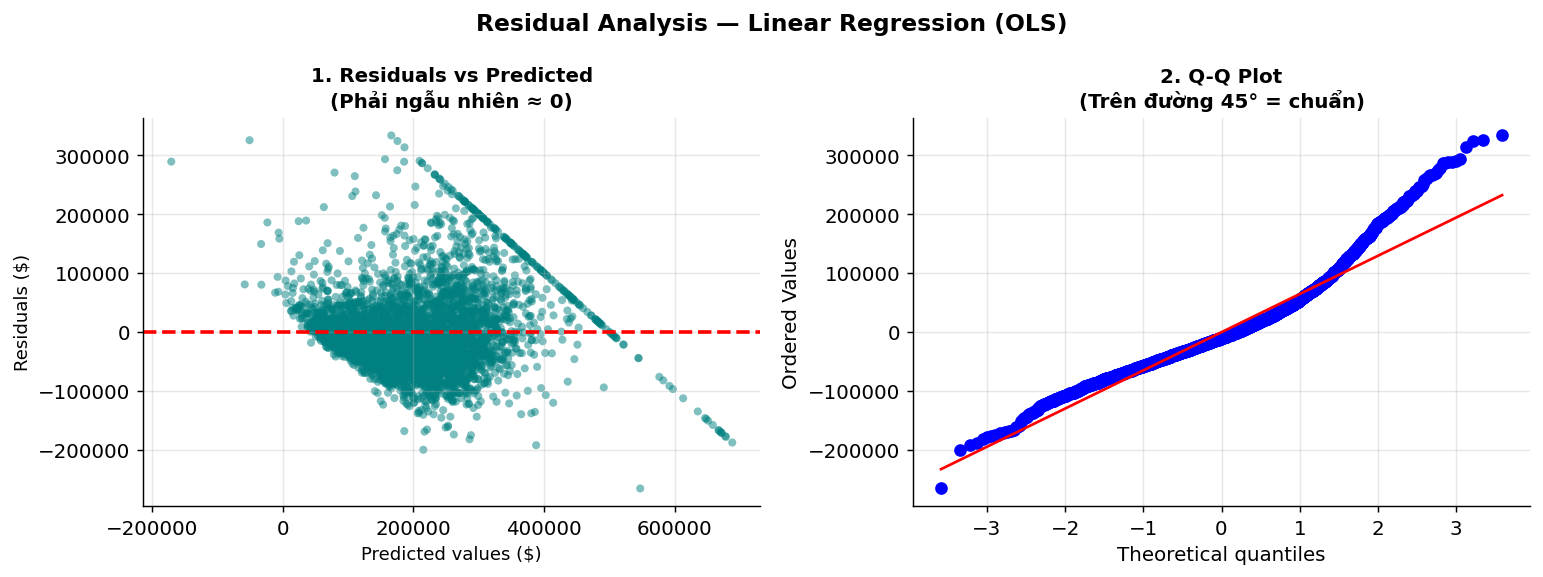
\includegraphics[width=\textwidth]{figures/regression_outputs/residual_ols.png}
  \caption{Residual Analysis -- Linear Regression (OLS).}
  \label{fig:residual_ols}
\end{figure}

\begin{table}[H]
  \centering
  \caption{Kết quả Breusch--Pagan test và Shapiro--Wilk test.}
  \label{tab:bp_sw_test}
  \begin{tabular}{llccc}
    \toprule
    \textbf{Kiểm định} & \textbf{Giả thuyết $H_0$} 
      & \textbf{Thống kê} & $p$-value & \textbf{Kết luận} \\
    \midrule
    Breusch--Pagan
      & Phương sai đồng nhất
      & $LM = 178.54$
      & $< 0.001$
      & Bác bỏ $H_0$ \\
    Shapiro--Wilk ($n=2{,}000$)
      & Phần dư chuẩn
      & $W = 0.8976$
      & $< 0.001$
      & Bác bỏ $H_0$ \\
    \bottomrule
  \end{tabular}
\end{table}

Nhận xét:
\begin{itemize}
  \item \textbf{Breusch--Pagan:} $p < 0.001$ -- bác bỏ $H_0$,
        phát hiện \textbf{heteroscedasticity}. Residual plot xác nhận:
        phương sai phần dư tăng theo giá trị dự báo, đặc biệt rõ ở
        vùng predicted $> \$300{,}000$ -- liên quan đến hiệu ứng capping
        tại \$500{,}001.
  \item \textbf{Shapiro--Wilk:} $W = 0.8976$, $p < 0.001$ -- phần dư
        \textbf{không phân phối chuẩn}; QQ-plot cho thấy đuôi nặng
        (heavy tails) ở cả hai phía.
  \item Do phát hiện heteroscedasticity, nhóm áp dụng
        \textbf{Weighted Least Squares (WLS)} với
        $w_n = 1/(|\hat{\epsilon}_n| + 10^{-5})$.
\end{itemize}

\subsubsection{Weighted Least Squares (WLS)}

\begin{figure}[H]
  \centering
  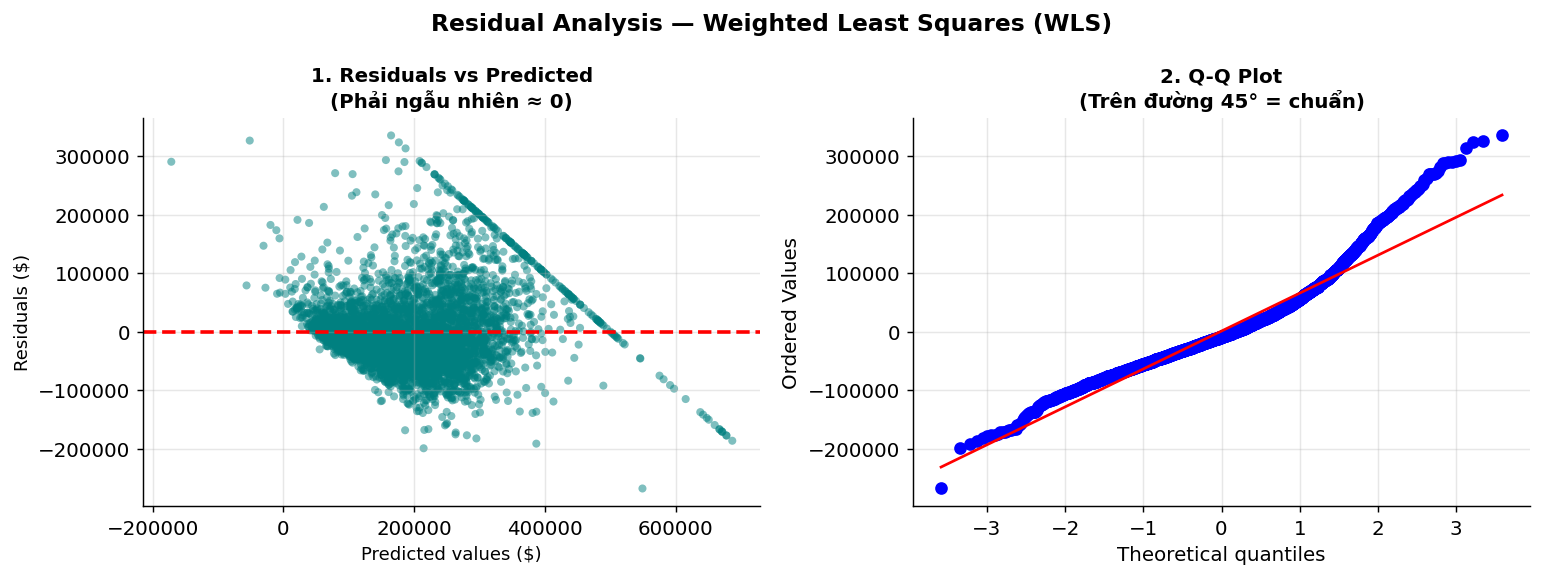
\includegraphics[width=\textwidth]{figures/regression_outputs/residual_wls.png}
  \caption{Residual Analysis -- Weighted Least Squares (WLS).}
  \label{fig:residual_wls}
\end{figure}

\begin{figure}[H]
  \centering
  \begin{subfigure}[b]{0.48\textwidth}
    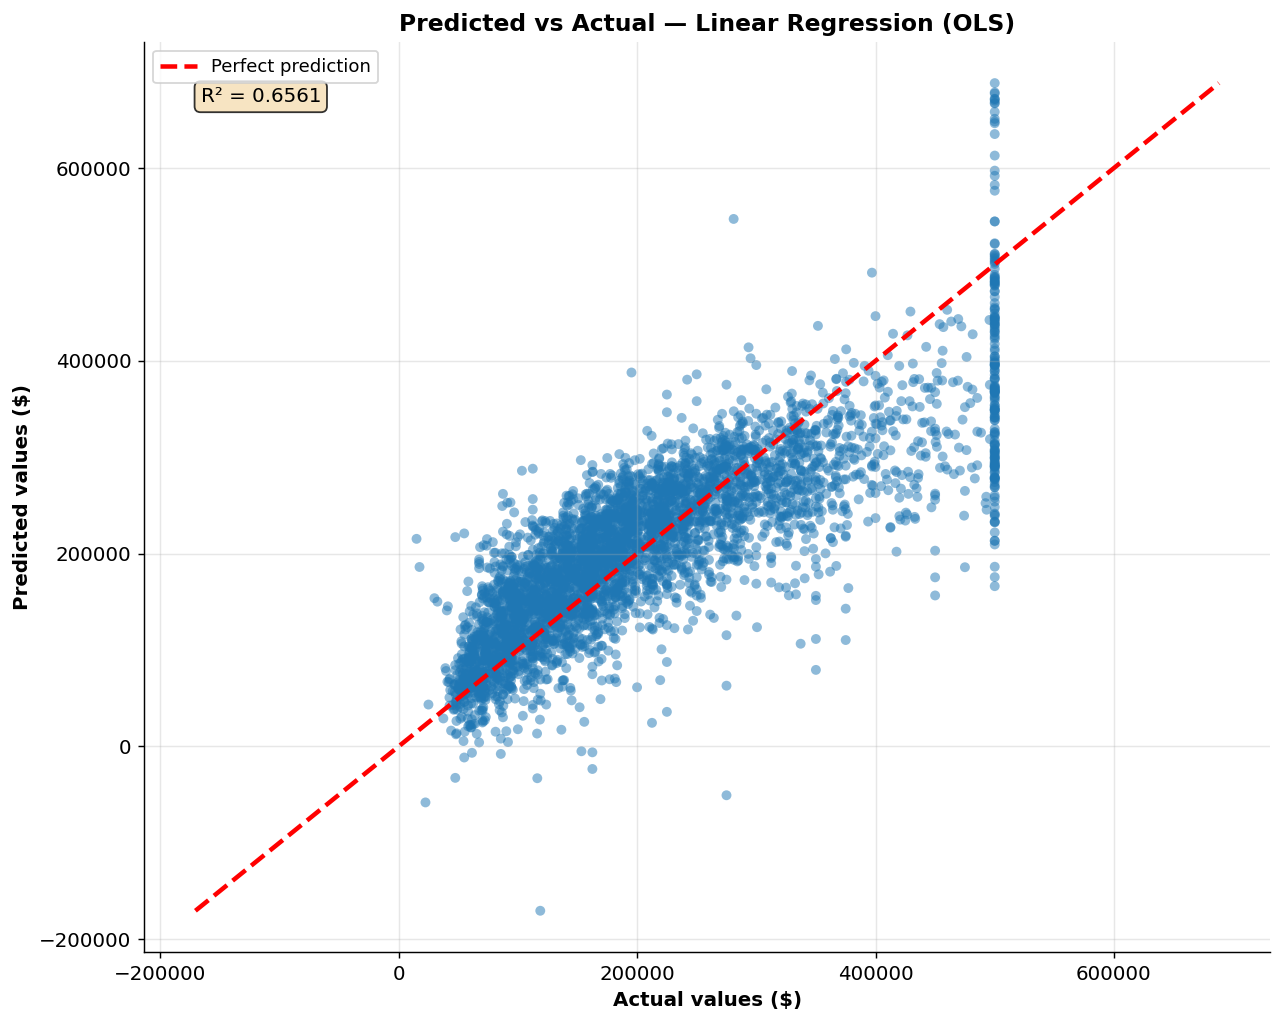
\includegraphics[width=\textwidth]{figures/regression_outputs/pred_actual_ols.png}
    \caption{OLS ($R^2 = 0.6561$)}
  \end{subfigure}
  \hfill
  \begin{subfigure}[b]{0.48\textwidth}
    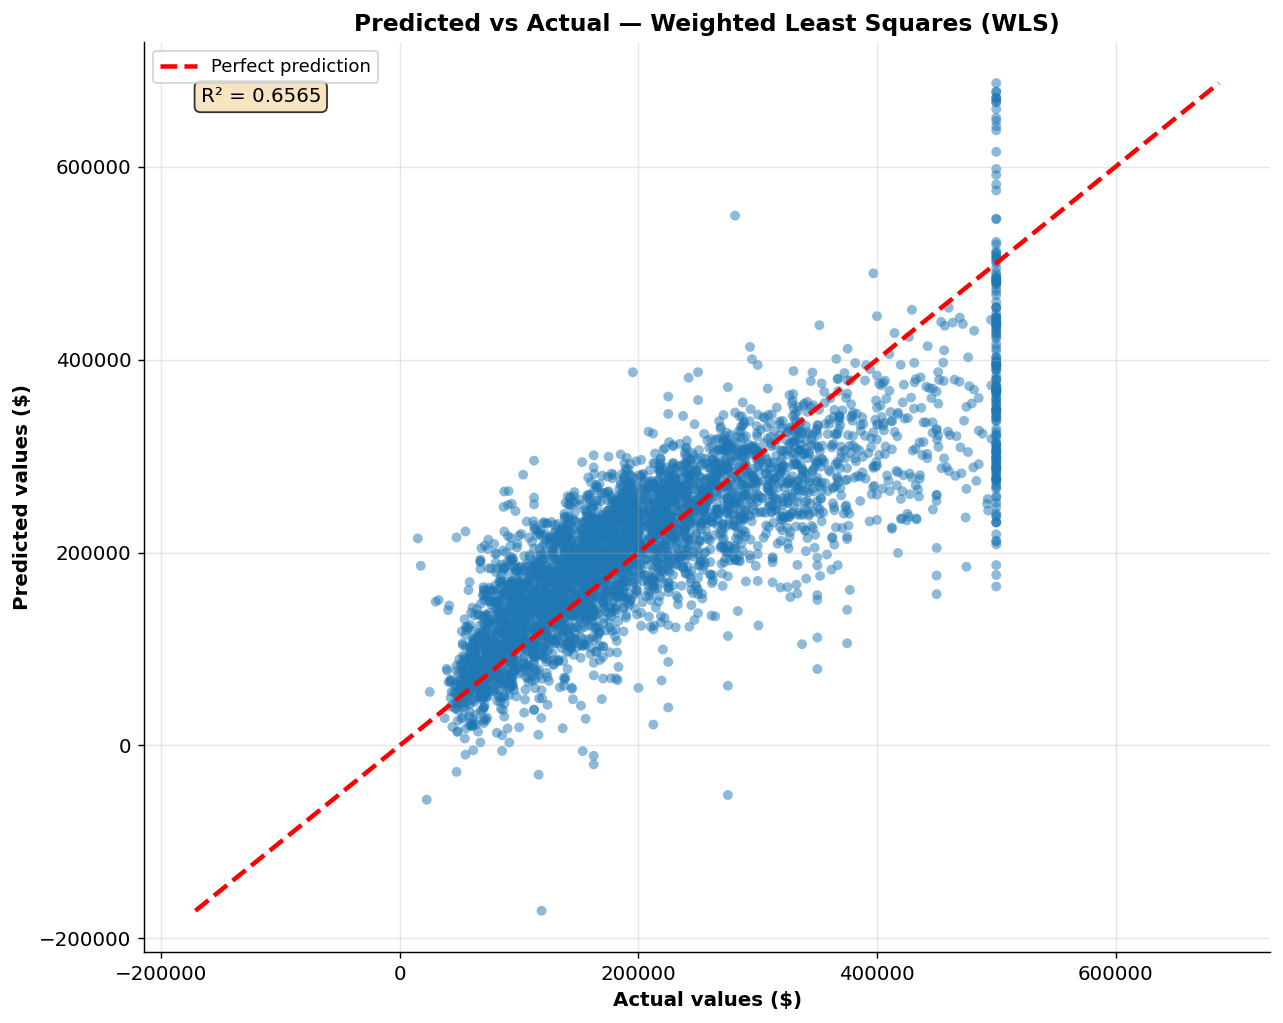
\includegraphics[width=\textwidth]{figures/regression_outputs/pred_actual_wls.png}
    \caption{WLS ($R^2 = 0.6565$)}
  \end{subfigure}
  \caption{Predicted vs.\ Actual -- OLS và WLS trên tập test.}
  \label{fig:pred_actual_ols_wls}
\end{figure}

\subsubsection{Learning Curve -- OLS}

\begin{figure}[H]
  \centering
  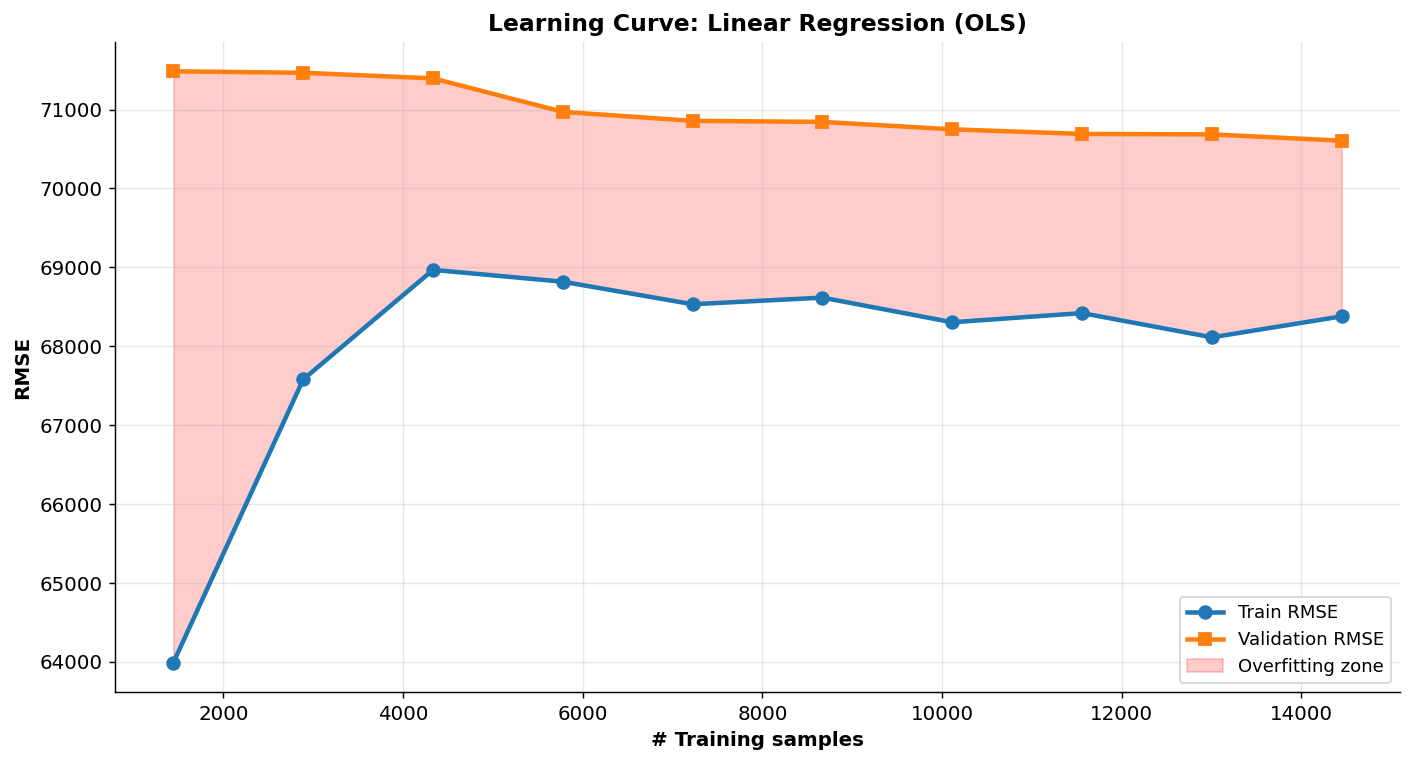
\includegraphics[width=0.80\textwidth]{figures/regression_outputs/learning_curve_ols.png}
  \caption{Learning curve -- Linear Regression (OLS):
           Train RMSE và Validation RMSE theo số mẫu huấn luyện.}
  \label{fig:lc_ols}
\end{figure}

Nhận xét: Train RMSE cuối $= \$68{,}379$, Val RMSE cuối $= \$70{,}605$,
overfitting gap $= \$2{,}226$ -- khoảng cách nhỏ, mô hình không overfit
nghiêm trọng. Cả hai đường hội tụ từ $\approx 10{,}000$ mẫu,
cho thấy OLS đã khai thác đủ thông tin với lượng dữ liệu hiện có.

\subsubsection{Kết quả trên tập Test}

\begin{table}[H]
  \centering
  \caption{So sánh OLS và WLS trên tập test.}
  \label{tab:ols_wls_test}
  \resizebox{\textwidth}{!}{%
  \begin{tabular}{lcccc}
    \toprule
    \textbf{Mô hình} & \textbf{MSE} & \textbf{RMSE} & \textbf{MAE} & $\mathbf{R^2}$ \\
    \midrule
    Linear Regression (OLS)
      & $4.482 \times 10^9$ & $\$66{,}948$ & $\$49{,}228$ & $0.6561$ \\
    Weighted Least Squares (WLS)
      & $4.477 \times 10^9$ & $\$66{,}912$ & $\$48{,}878$ & $0.6565$ \\
    \bottomrule
  \end{tabular}}
\end{table}

\begin{table}[H]
  \centering
  \caption{10-Fold CV -- Linear Regression (OLS).}
  \label{tab:ols_cv}
  \begin{tabular}{lcc}
    \toprule
    \textbf{Chỉ số} & \textbf{Mean} & \textbf{Std} \\
    \midrule
    MSE  & $4{,}739{,}322{,}093$ & $415{,}799{,}254$ \\
    RMSE & $\$68{,}778$          & $\$2{,}978$       \\
    MAE  & $\$49{,}503$          & $\$872$           \\
    $R^2$& $0.6441$              & $0.0314$          \\
    \bottomrule
  \end{tabular}
\end{table}

\begin{table}[H]
  \centering
  \caption{Kiểm định thống kê OLS vs.\ WLS trên tập test ($\alpha = 0.05$).}
  \label{tab:ols_wls_stat}
  \begin{tabular}{llccc}
    \toprule
    \textbf{Kiểm định} & \textbf{Cặp so sánh}
      & \textbf{Thống kê} & $p$-value & \textbf{Kết luận} \\
    \midrule
    Paired $t$-test
      & OLS vs.\ WLS & $t = 11.224$ & $< 0.001$
      & WLS tốt hơn có ý nghĩa \\
    Wilcoxon
      & OLS vs.\ WLS & $W = 3{,}300{,}624$ & $< 0.001$
      & WLS tốt hơn có ý nghĩa \\
    \bottomrule
  \end{tabular}
\end{table}

Nhận xét:
\begin{itemize}
  \item \textbf{WLS cải thiện nhẹ so với OLS}: RMSE giảm $\$36$
        ($-0.05\%$), MAE giảm $\$350$ ($-0.7\%$), $R^2$ tăng $0.0004$.
        Cả Paired $t$-test và Wilcoxon đều cho $p < 0.001$, xác nhận
        sự khác biệt có ý nghĩa thống kê -- dù mức cải thiện thực tế
        rất nhỏ.
  \item Lý do WLS cải thiện không nhiều: heteroscedasticity chủ yếu
        đến từ hiệu ứng \emph{capping} tại \$500{,}001 (một cấu trúc
        dữ liệu đặc thù), không phải từ phi tuyến tính thực sự của
        quan hệ giữa features và target.
  \item $R^2 \approx 0.656$ cho thấy mô hình tuyến tính giải thích
        được $65.6\%$ phương sai giá nhà -- còn $34.4\%$ chưa được
        bắt, gợi ý cần các mô hình phi tuyến phức tạp hơn.
\end{itemize}

% -----------------------------------------------------------
\subsection{Hồi quy có Regularization và Lựa chọn Đặc trưng}
\label{ssec:regularization}

\subsubsection{Chọn $\lambda$ tối ưu bằng 10-Fold CV và Grid Search}

Grid search trên 50 giá trị $\lambda \in [10^{-4}, 10^4]$ (log scale),
kết hợp Lasso Path (warm-start) cho Lasso:

\begin{table}[H]
  \centering
  \caption{Kết quả chọn $\lambda^*$ bằng 10-Fold CV.}
  \label{tab:best_lambda}
  \begin{tabular}{lcc}
    \toprule
    \textbf{Mô hình} & \textbf{Best $\lambda^*$} & \textbf{CV RMSE} \\
    \midrule
    Ridge (Grid Search)       & $35.5648$ & $\$68{,}758$ \\
    Lasso (Warm-start Path)   & $232.9952$ & $\$68{,}798$ \\
    \bottomrule
  \end{tabular}
\end{table}

Lasso cần $\lambda^*$ lớn hơn Ridge đáng kể ($232.99$ vs.\ $35.56$) vì
penalty L1 tác động theo đơn vị tuyệt đối của hệ số, trong khi L2 theo
bình phương -- cùng mức co hệ số đòi hỏi $\lambda$ lớn hơn với L1.

\subsubsection{Regularization Path}

\begin{figure}[H]
  \centering
  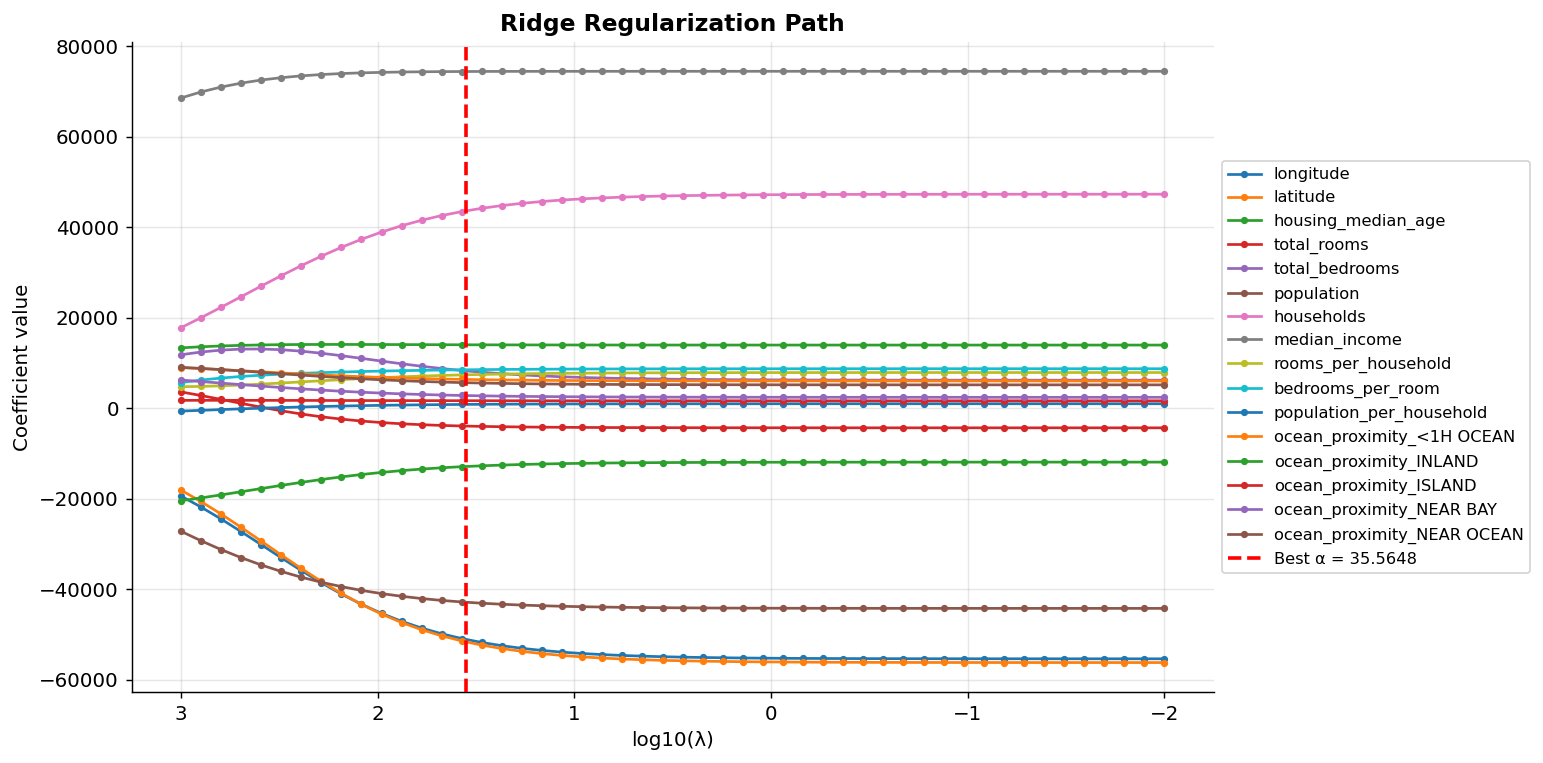
\includegraphics[width=\textwidth]{figures/regression_outputs/ridge_path.png}
  \caption{Ridge Regularization Path: hệ số $w_j$ theo $\log_{10}(\lambda)$.
           Đường đỏ: $\lambda^* = 35.56$.}
  \label{fig:ridge_path}
\end{figure}

\begin{figure}[H]
  \centering
  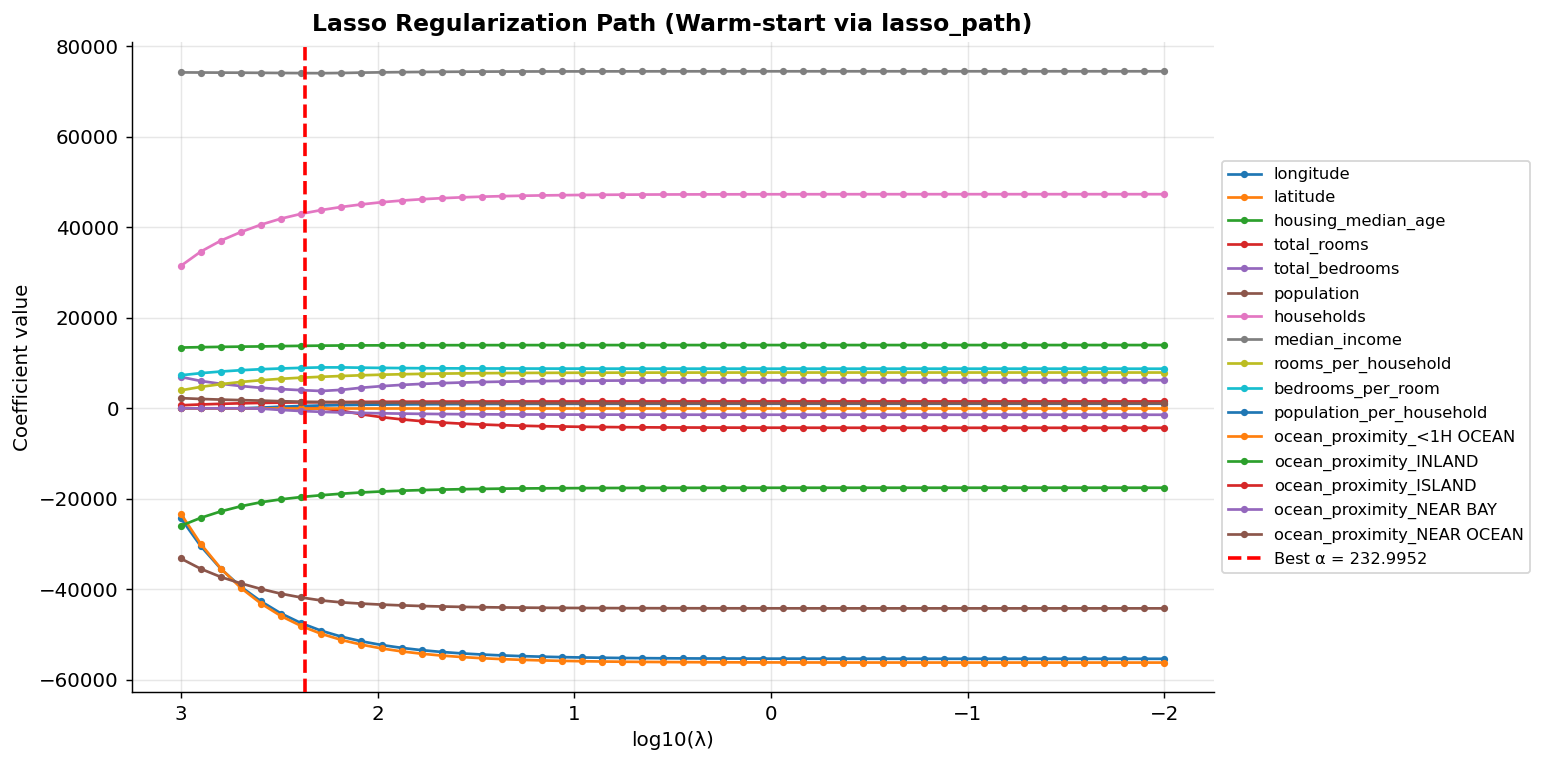
\includegraphics[width=\textwidth]{figures/regression_outputs/lasso_path.png}
  \caption{Lasso Regularization Path (warm-start): hệ số $w_j$ theo
           $\log_{10}(\lambda)$. Đường đỏ: $\lambda^* = 233.00$.}
  \label{fig:lasso_path}
\end{figure}

Nhận xét:
\begin{itemize}
  \item \textbf{Ridge}: Tất cả hệ số co dần về 0 khi $\lambda$ tăng
        nhưng \textbf{không triệt tiêu hẳn} -- đặc tính của L2.
        \texttt{median\_income} (xám) và \texttt{households} (hồng)
        duy trì giá trị lớn nhất qua toàn bộ path, xác nhận đây là
        hai đặc trưng quan trọng nhất.
  \item \textbf{Lasso}: Nhiều hệ số bị đưa về đúng 0 khi $\lambda$
        tăng -- đặc tính sparsity của L1. Tại $\lambda^* = 233.00$,
        Lasso giữ lại 14/16 đặc trưng (loại 2 đặc trưng ít quan trọng).
  \item Nhóm \texttt{longitude}, \texttt{latitude} và
        \texttt{ocean\_proximity\_*} có hệ số âm lớn -- phản ánh tác
        động địa lý và vị trí ven biển đến giá nhà.
\end{itemize}

\subsubsection{Elastic Net}

\begin{figure}[H]
  \centering
  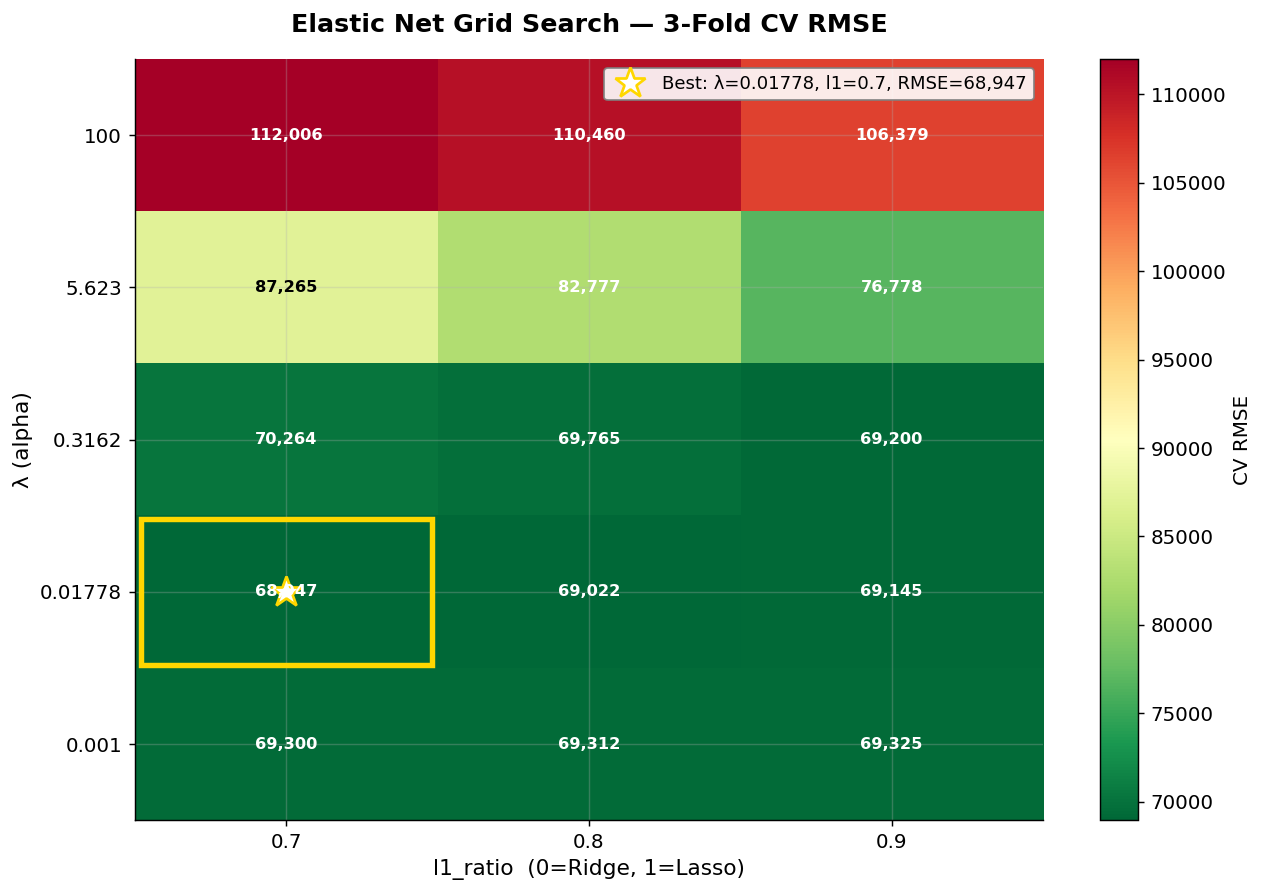
\includegraphics[width=0.75\textwidth]{figures/regression_outputs/elasticnet_heatmap.png}
  \caption{Elastic Net Grid Search -- 3-Fold CV RMSE theo
           $(\lambda, \text{l1\_ratio})$.}
  \label{fig:elasticnet_heatmap}
\end{figure}

Cấu hình tối ưu: $\lambda^* = 0.01778$, \texttt{l1\_ratio} $= 0.70$,
CV RMSE $= \$68{,}947$.

Quy đổi sang ký hiệu \eqref{eq:elasticnet}:
\begin{align*}
  \lambda_1 &= \lambda \cdot \text{l1\_ratio} = 0.01778 \times 0.7 = 0.01245 \\
  \lambda_2 &= \frac{\lambda \cdot (1 - \text{l1\_ratio})}{2}
             = \frac{0.01778 \times 0.3}{2} = 0.00267
\end{align*}

Nhận xét: Vùng tối ưu nằm ở \textbf{$\lambda$ nhỏ} (regularization yếu)
và \textbf{l1\_ratio $= 0.7$} (thiên về L1), cho thấy mô hình hưởng lợi
từ tính chọn lọc đặc trưng của L1 nhưng vẫn cần L2 để ổn định hóa các
hệ số tương quan cao (do multicollinearity đã quan sát ở Mục~\ref{sec:eda}).

\subsubsection{Lựa chọn đặc trưng}

\begin{figure}[H]
  \centering
  
\includegraphics[width=\textwidth]{figures/regression_outputs/feature_selection.png}
  \caption{So sánh 3 chiến lược lựa chọn đặc trưng: số features chọn (trái)
           và Validation RMSE (phải).}
  \label{fig:feature_selection}
\end{figure}

\begin{table}[H]
  \centering
  \caption{So sánh các chiến lược lựa chọn đặc trưng.}
  \label{tab:feature_selection}
  \begin{tabular}{lccl}
    \toprule
    \textbf{Phương pháp} & \textbf{Số features} & \textbf{Val RMSE} & \textbf{Nhận xét} \\
    \midrule
    Forward Stepwise   & 16 & $\$68{,}981$ & Giữ tất cả (greedy add) \\
    Backward Elimination & 1 & $\$83{,}644$ & Chỉ giữ 1 feature \\
    Lasso-based        & 14 & $\$70{,}603$ & Loại 2 features ít quan trọng \\
    \bottomrule
  \end{tabular}
\end{table}

Nhận xét:
\begin{itemize}
  \item \textbf{Forward Stepwise} giữ toàn bộ 16 features và đạt Val
        RMSE tốt nhất ($\$68{,}981$) -- trên bộ dữ liệu này tất cả
        features đều đóng góp thông tin.
  \item \textbf{Backward Elimination} chỉ giữ lại 1 feature, RMSE tăng
        vọt lên $\$83{,}644$ ($+21\%$) -- thuật toán greedy bị kẹt ở
        local optimum khi loại feature theo p-value trên dữ liệu có
        multicollinearity cao.
  \item \textbf{Lasso-based} loại 2/16 features (sparsity $= 12.5\%$),
        Val RMSE $= \$70{,}603$ -- tự động và không greedy, cho kết quả
        cân bằng giữa model complexity và hiệu năng.
\end{itemize}

\subsubsection{Learning Curves}

\begin{figure}[H]
  \centering
  \begin{subfigure}[b]{0.48\textwidth}
    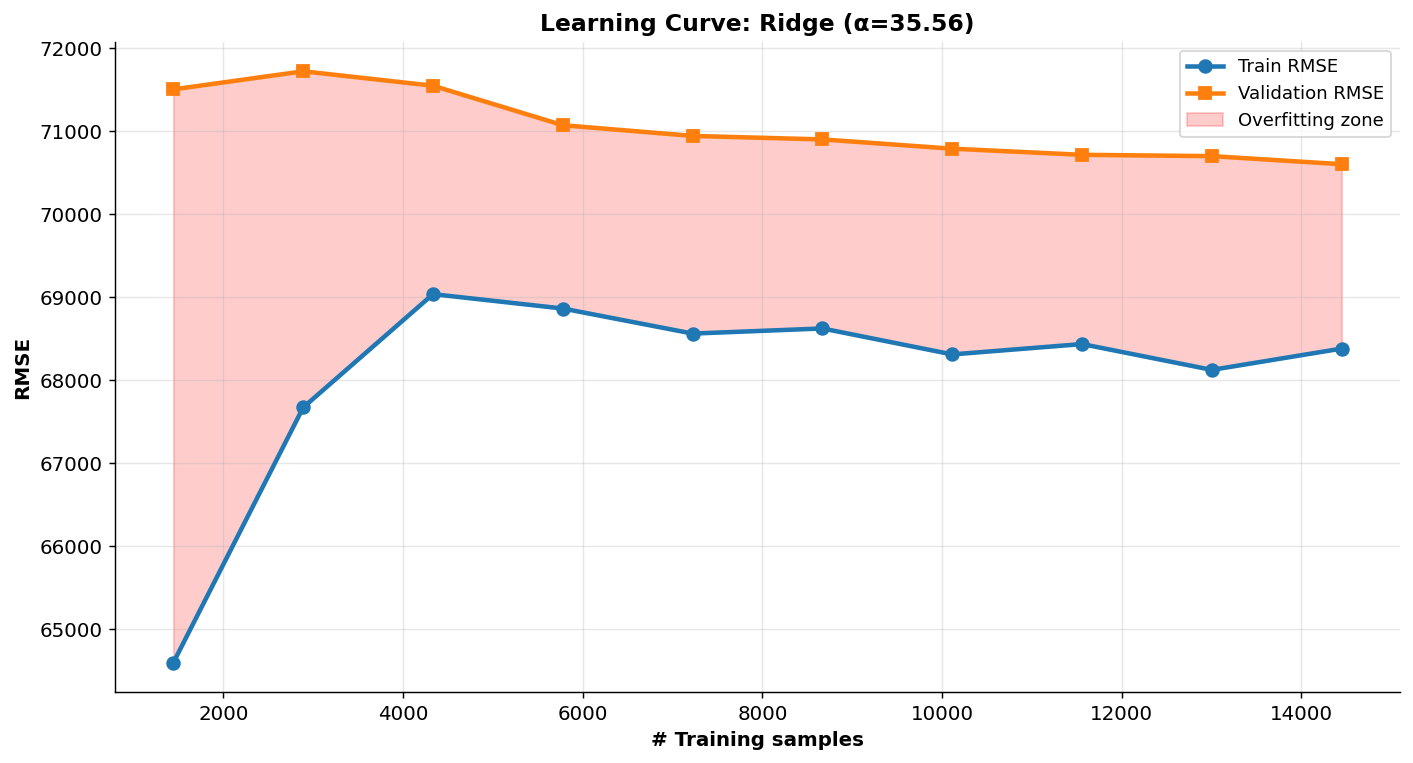
\includegraphics[width=\textwidth]{figures/regression_outputs/lc_ridge.png}
    \caption{Ridge ($\alpha=35.56$)}
  \end{subfigure}
  \hfill
  \begin{subfigure}[b]{0.48\textwidth}
    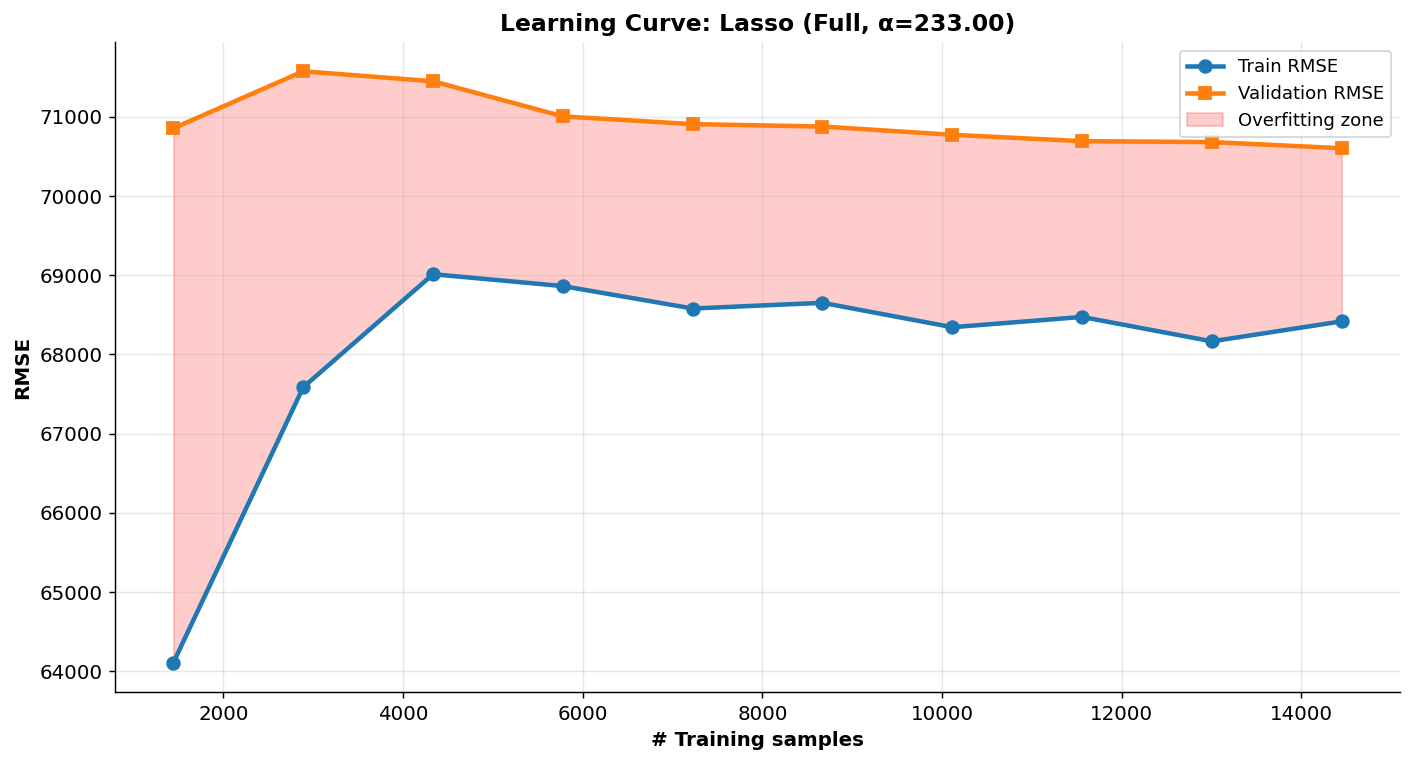
\includegraphics[width=\textwidth]{figures/regression_outputs/lc_lasso_full.png}
    \caption{Lasso Full ($\alpha=233.00$)}
  \end{subfigure}

  \begin{subfigure}[b]{0.48\textwidth}
    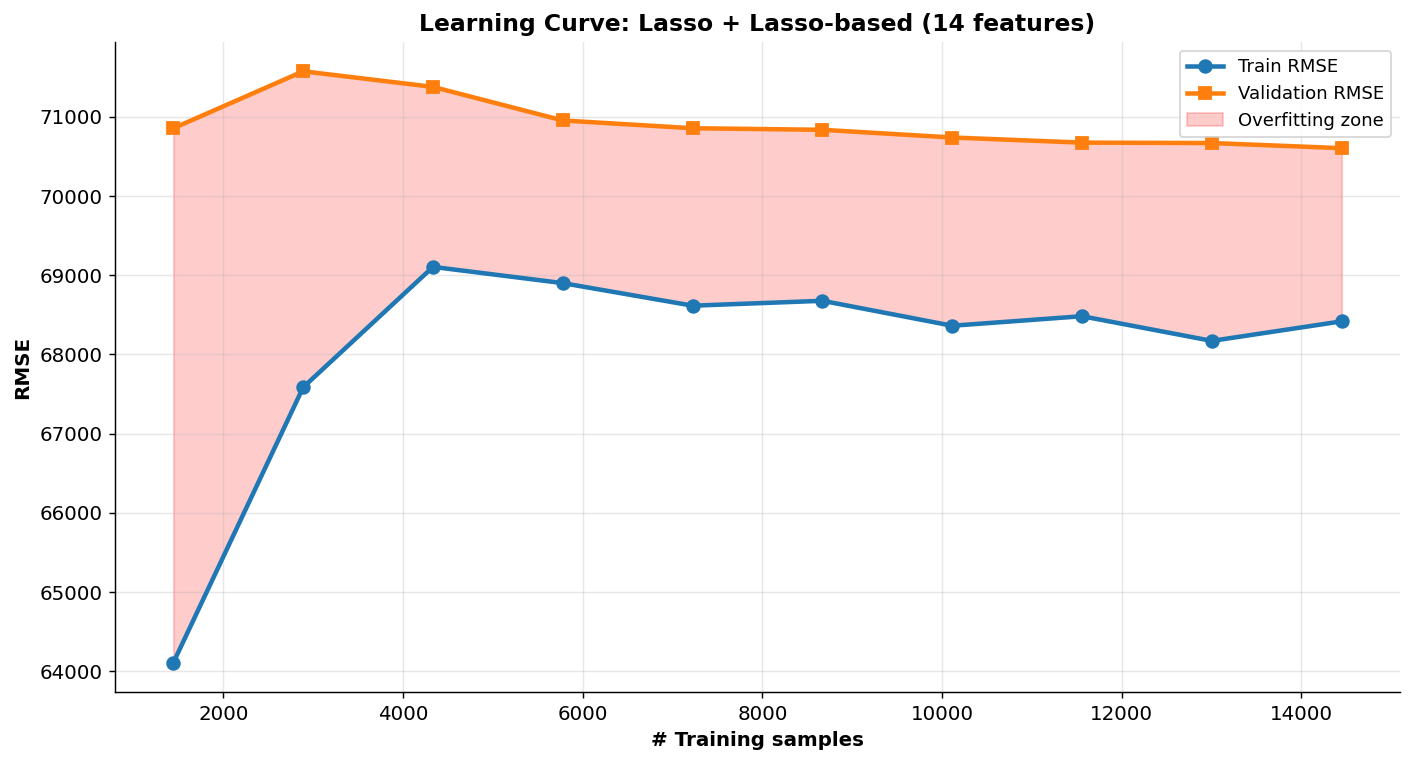
\includegraphics[width=\textwidth]{figures/regression_outputs/lc_lasso_selected.png}
    \caption{Lasso + Lasso-based (14 features)}
  \end{subfigure}
  \hfill
  \begin{subfigure}[b]{0.48\textwidth}
    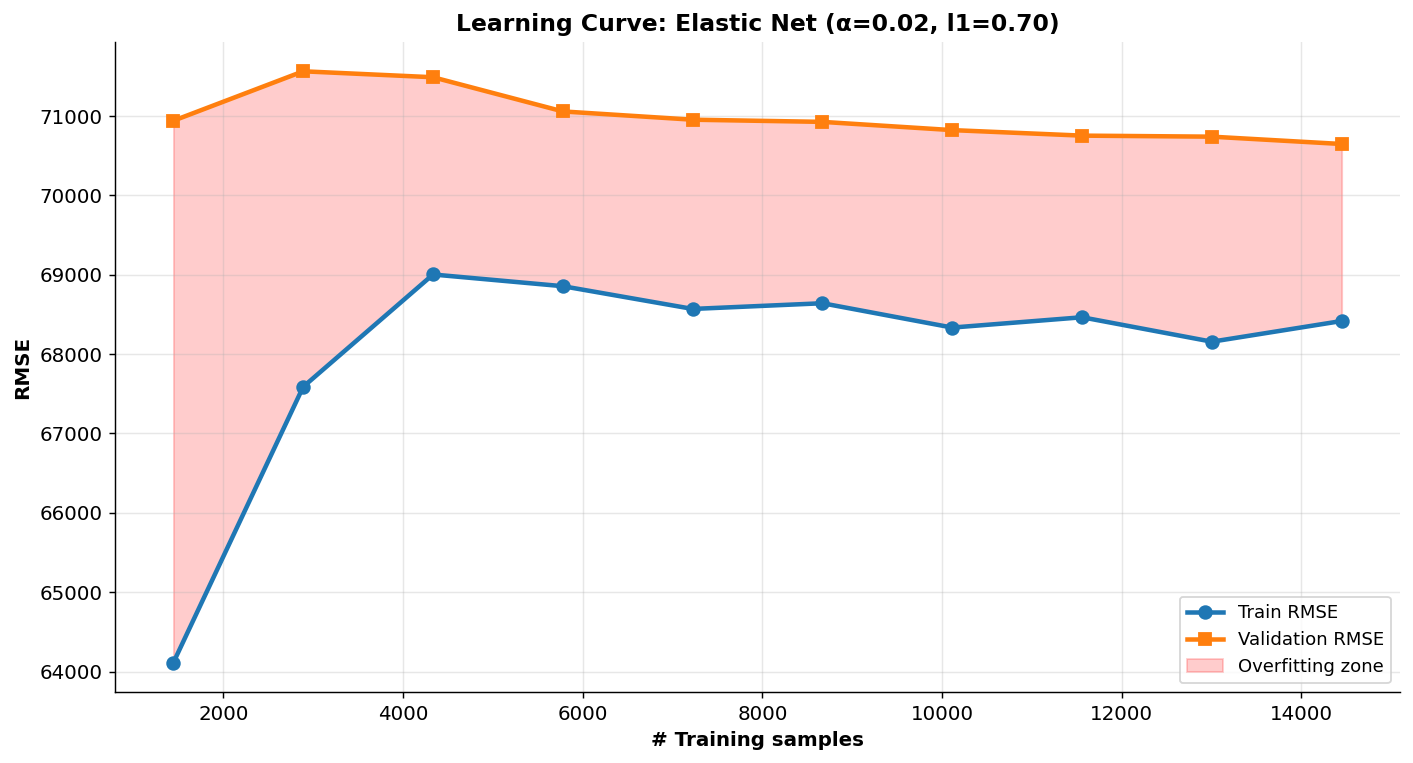
\includegraphics[width=\textwidth]{figures/regression_outputs/lc_elasticnet.png}
    \caption{Elastic Net ($\alpha=0.02$, l1$=0.70$)}
  \end{subfigure}
  \caption{Learning curves -- các mô hình Regularization.}
  \label{fig:lc_reg}
\end{figure}

\subsubsection{Residual Analysis}

\begin{figure}[H]
  \centering
  \begin{subfigure}[b]{0.48\textwidth}
    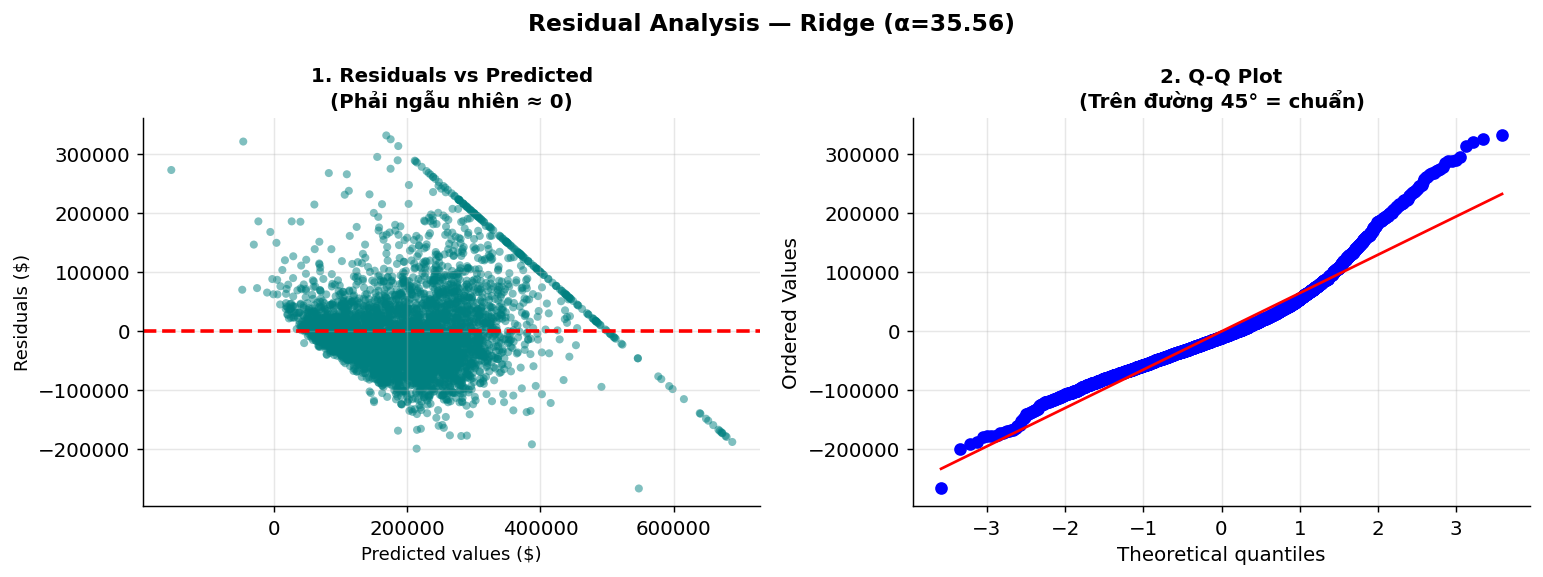
\includegraphics[width=\textwidth]{figures/regression_outputs/residual_ridge.png}
    \caption{Ridge ($\alpha=35.56$)}
  \end{subfigure}
  \hfill
  \begin{subfigure}[b]{0.48\textwidth}
    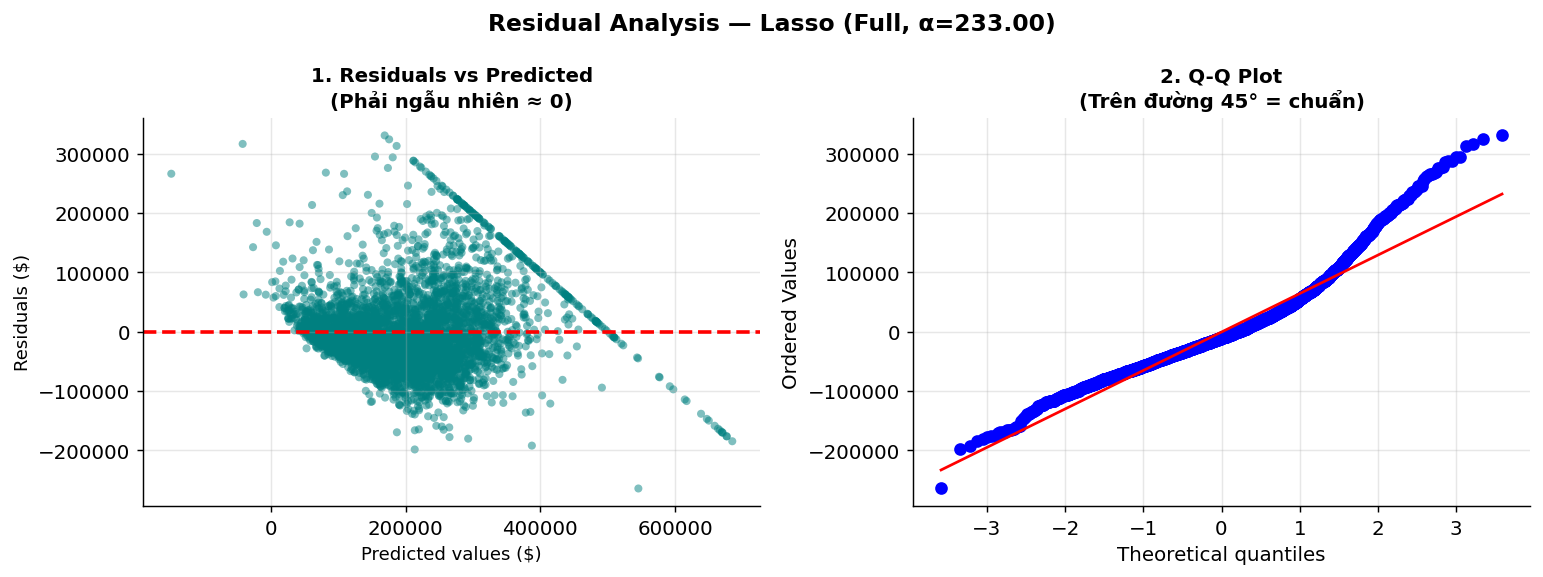
\includegraphics[width=\textwidth]{figures/regression_outputs/residual_lasso_full.png}
    \caption{Lasso Full ($\alpha=233.00$)}
  \end{subfigure}

  \begin{subfigure}[b]{0.48\textwidth}
    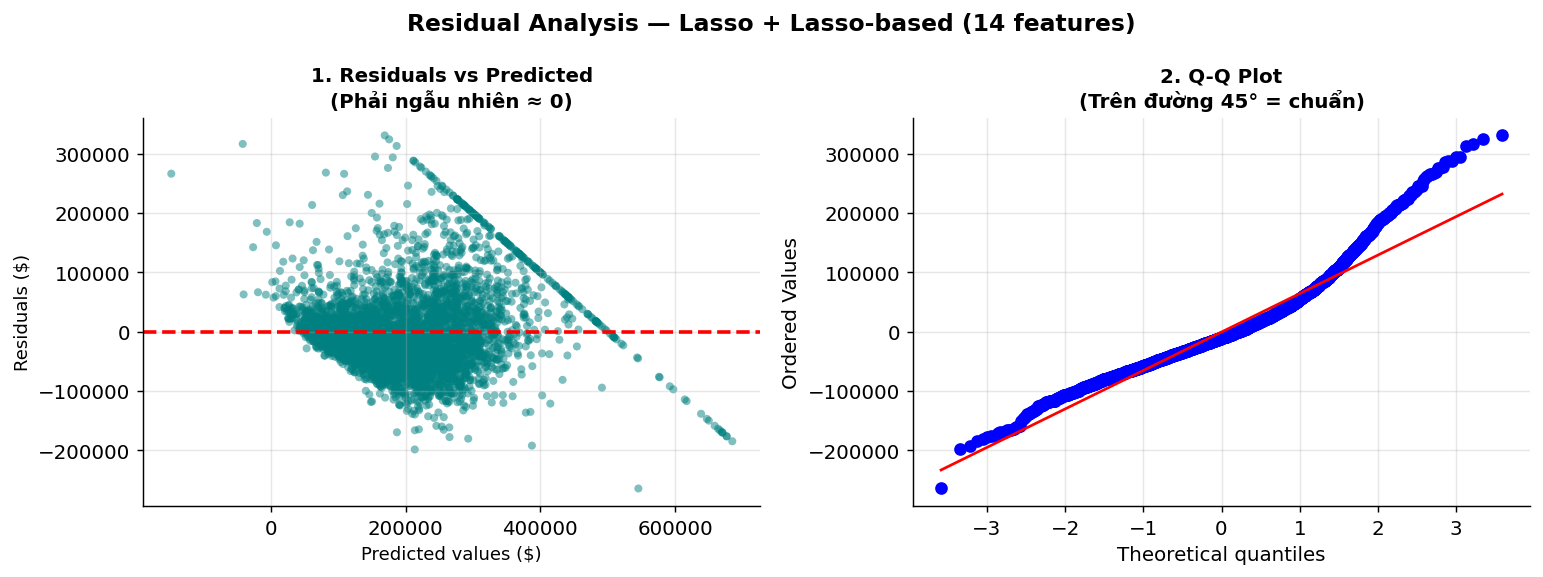
\includegraphics[width=\textwidth]{figures/regression_outputs/residual_lasso_selected.png}
    \caption{Lasso + Lasso-based (14 features)}
  \end{subfigure}
  \hfill
  \begin{subfigure}[b]{0.48\textwidth}
    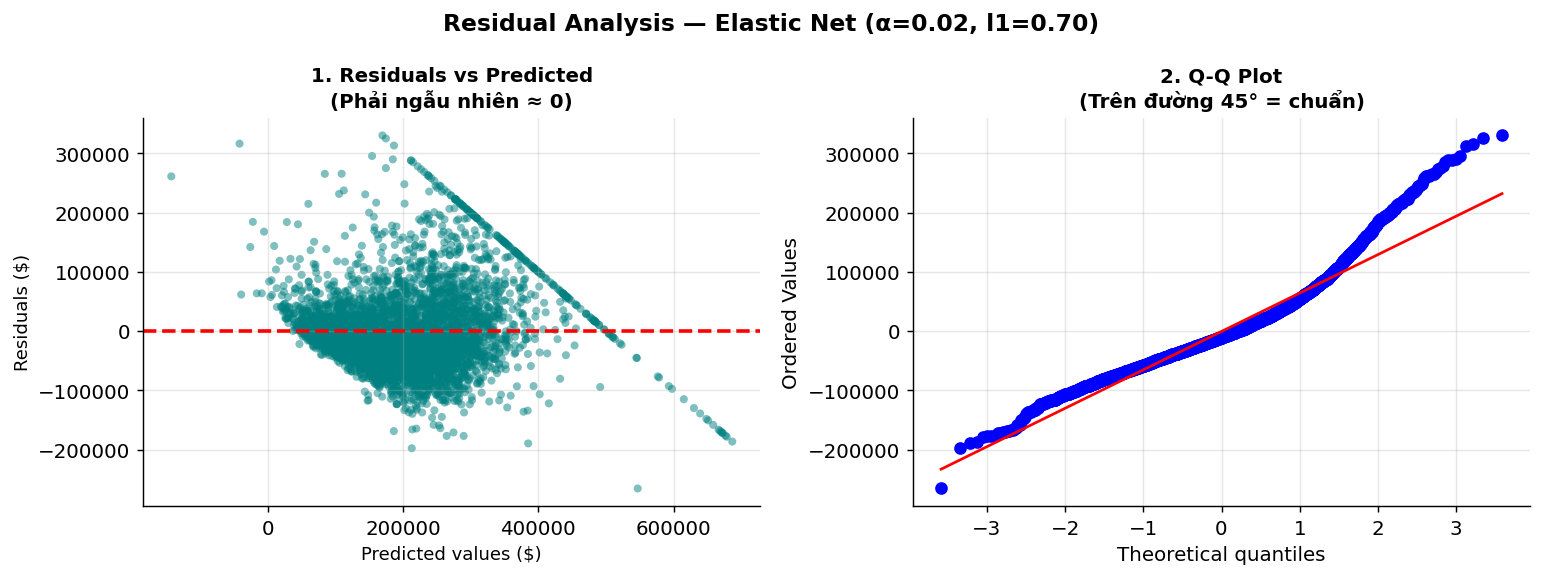
\includegraphics[width=\textwidth]{figures/regression_outputs/residual_elasticnet.png}
    \caption{Elastic Net ($\alpha=0.02$, l1$=0.70$)}
  \end{subfigure}
  \caption{Residual Analysis -- các mô hình Regularization trên tập test.}
  \label{fig:residual_reg}
\end{figure}

\subsubsection{Predicted vs.\ Actual}

\begin{figure}[H]
  \centering
  \begin{subfigure}[b]{0.48\textwidth}
    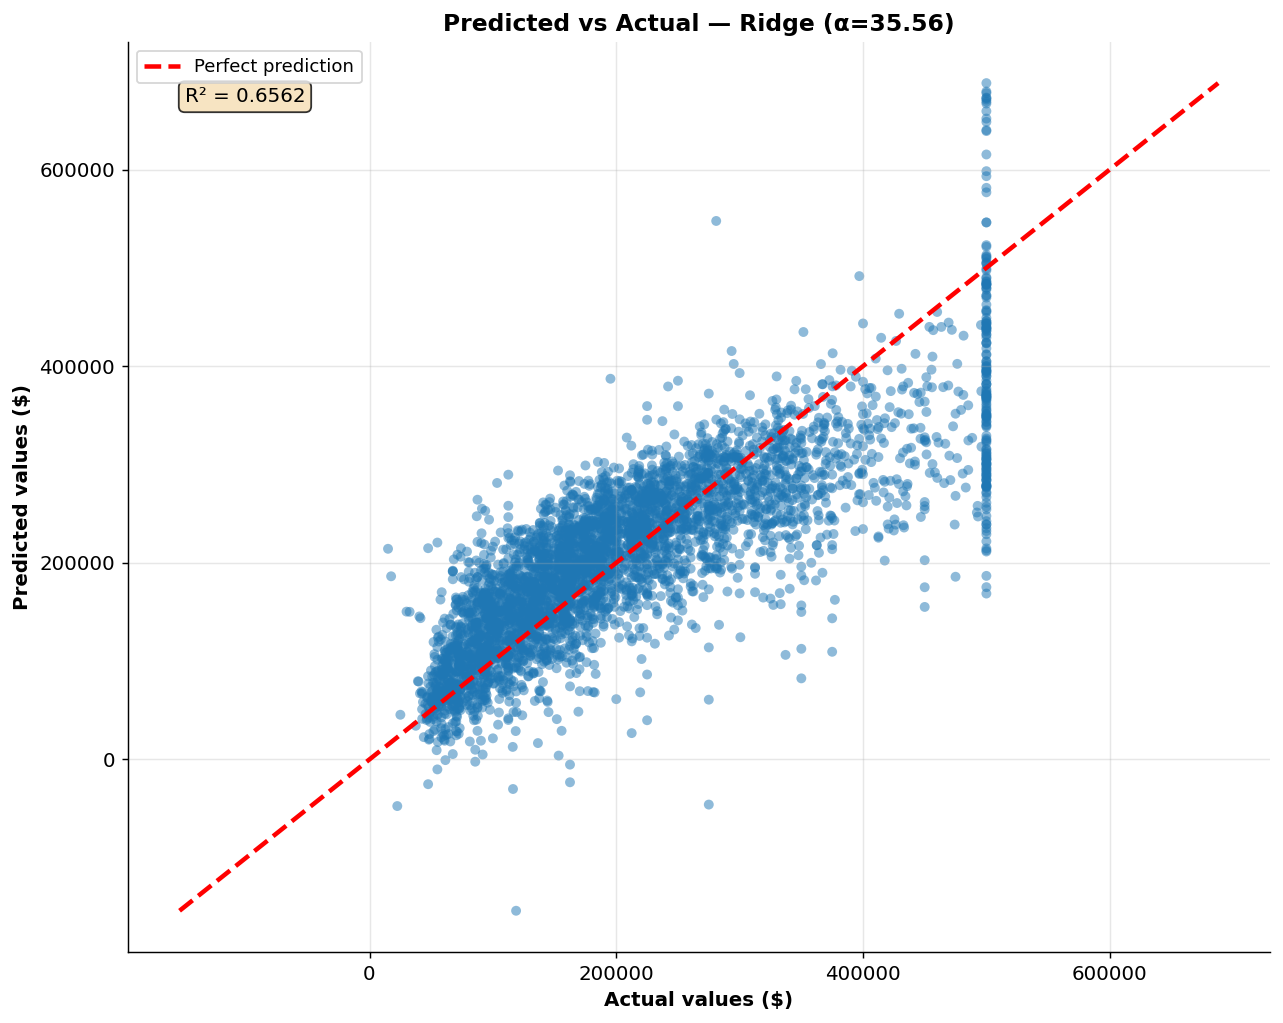
\includegraphics[width=\textwidth]{figures/regression_outputs/pred_actual_ridge.png}
    \caption{Ridge ($R^2 = 0.6562$)}
  \end{subfigure}
  \hfill
  \begin{subfigure}[b]{0.48\textwidth}
    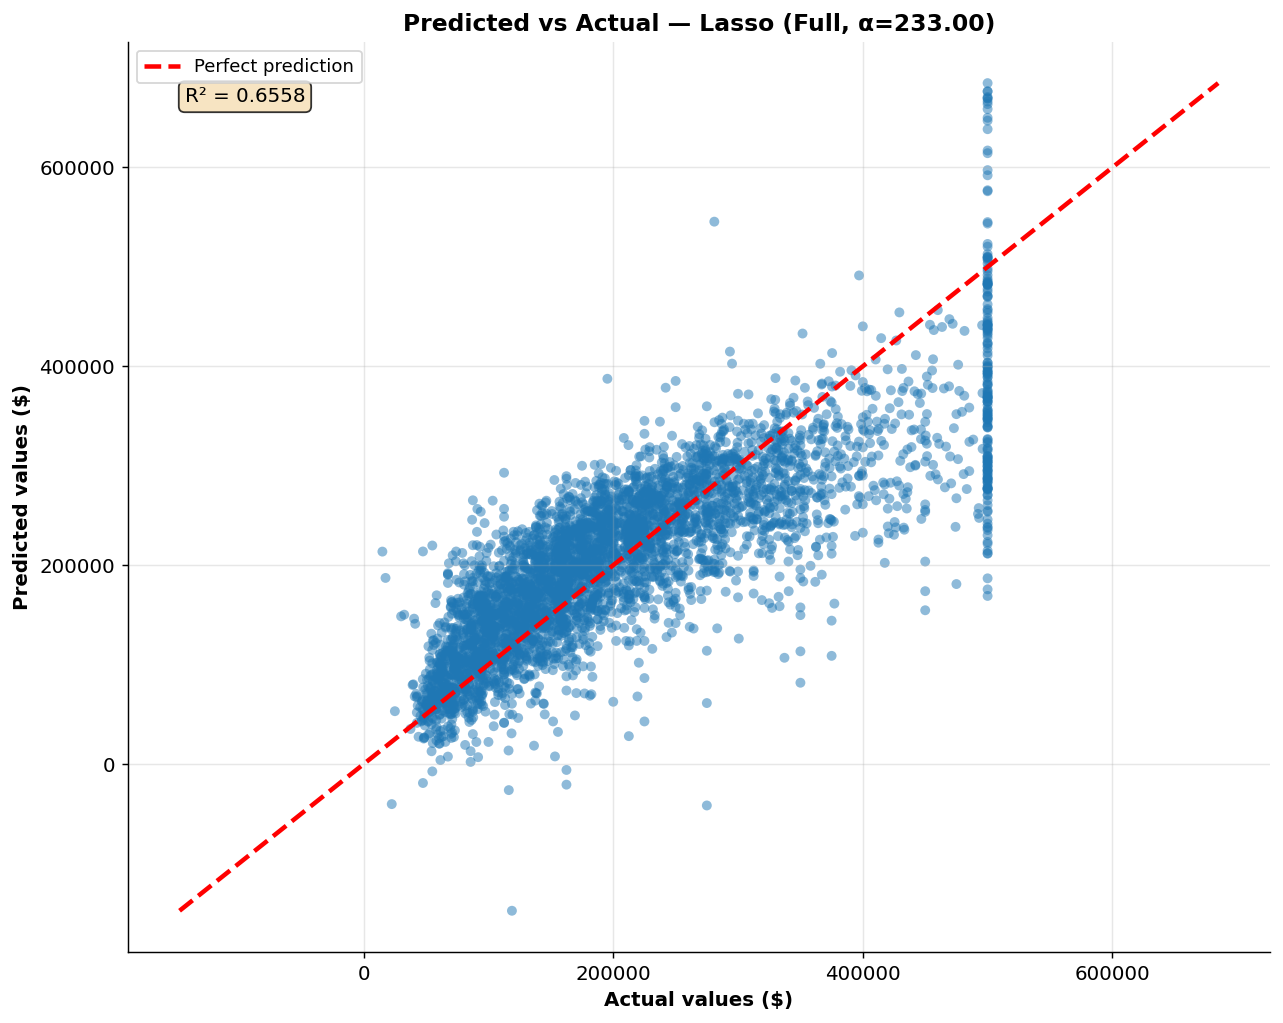
\includegraphics[width=\textwidth]{figures/regression_outputs/pred_actual_lasso_full.png}
    \caption{Lasso Full ($R^2 = 0.6558$)}
  \end{subfigure}

  \begin{subfigure}[b]{0.48\textwidth}
    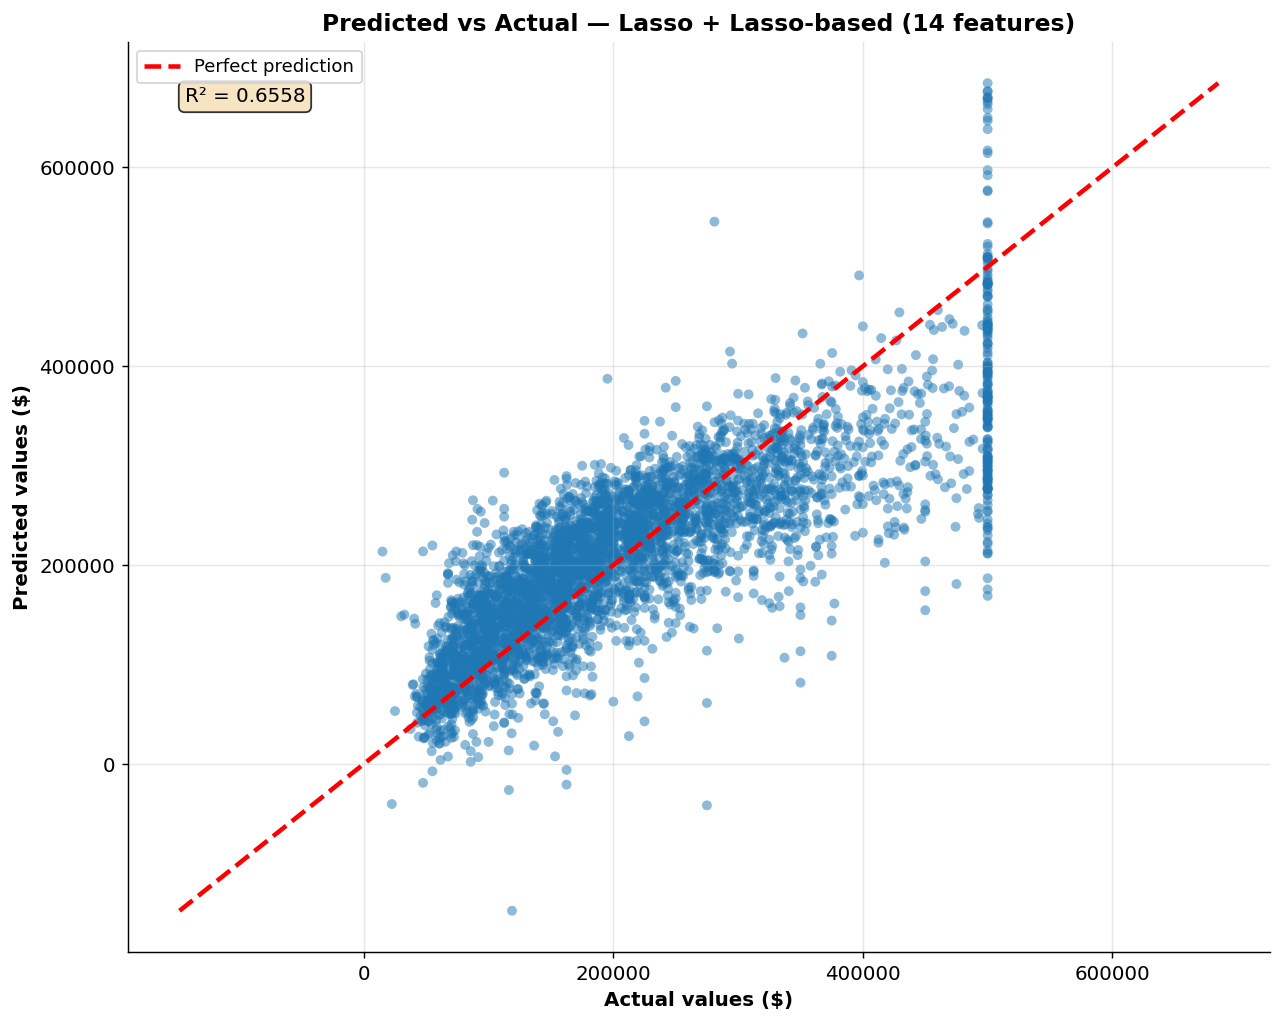
\includegraphics[width=\textwidth]{figures/regression_outputs/pred_actual_lasso_selected.png}
    \caption{Lasso + Lasso-based ($R^2 = 0.6558$)}
  \end{subfigure}
  \hfill
  \begin{subfigure}[b]{0.48\textwidth}
    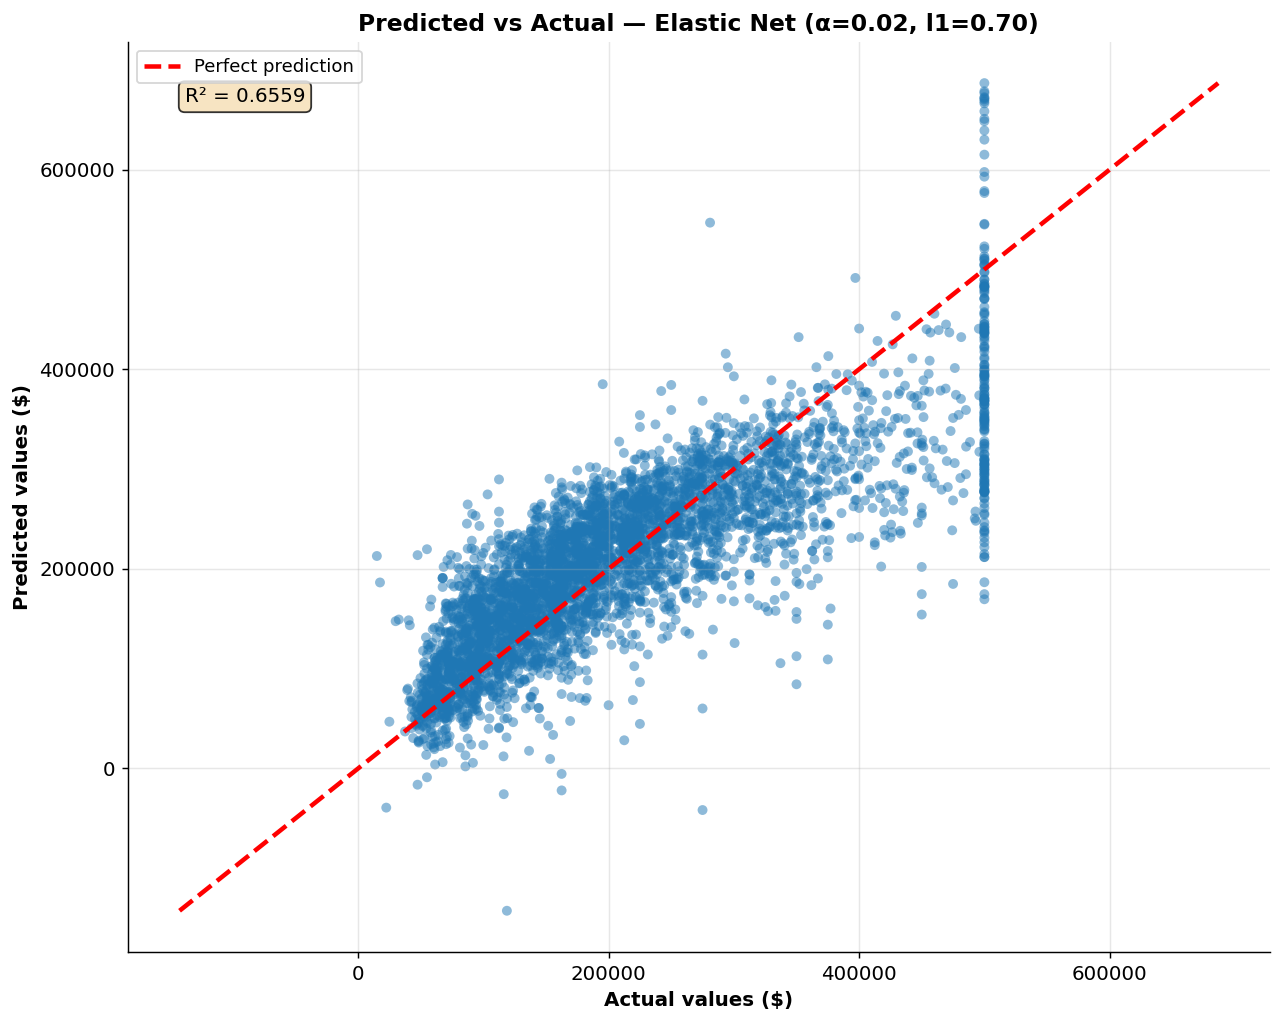
\includegraphics[width=\textwidth]{figures/regression_outputs/pred_actual_elasticnet.png}
    \caption{Elastic Net ($R^2 = 0.6559$)}
  \end{subfigure}
  \caption{Predicted vs.\ Actual -- các mô hình Regularization trên tập test.}
  \label{fig:pred_actual_reg}
\end{figure}

\subsubsection{Kết quả trên tập Test}

\begin{table}[H]
  \centering
  \caption{So sánh các mô hình Regularization trên tập test.}
  \label{tab:reg_test}
  \resizebox{\textwidth}{!}{%
  \begin{tabular}{lcccc}
    \toprule
    \textbf{Mô hình} & \textbf{MSE} & \textbf{RMSE} & \textbf{MAE} & $\mathbf{R^2}$ \\
    \midrule
    Ridge ($\alpha^* = 35.56$)
      & $4.480 \times 10^9$ & $\$66{,}936$ & $\$49{,}209$ & $0.6562$ \\
    Elastic Net ($\alpha=0.02$, l1$=0.70$)
      & $4.484 \times 10^9$ & $\$66{,}966$ & $\$49{,}216$ & $0.6559$ \\
    Lasso Full ($\alpha^* = 233.00$)
      & $4.486 \times 10^9$ & $\$66{,}974$ & $\$49{,}202$ & $0.6558$ \\
    Lasso + Lasso-based (14 features)
      & $4.486 \times 10^9$ & $\$66{,}974$ & $\$49{,}202$ & $0.6558$ \\
    \bottomrule
  \end{tabular}}
\end{table}

\begin{table}[H]
  \centering
  \caption{10-Fold CV (mean $\pm$ std) -- các mô hình Regularization.}
  \label{tab:reg_cv}
  \resizebox{\textwidth}{!}{%
  \begin{tabular}{lcccc}
    \toprule
    \textbf{Mô hình} & \textbf{RMSE} & \textbf{MAE} & $\mathbf{R^2}$ \\
    \midrule
    Ridge ($\alpha^*=35.56$)
      & $\$68{,}758 \pm \$2{,}900$ & $\$49{,}485 \pm \$907$ & $0.6444 \pm 0.0305$ \\
    Lasso Full ($\alpha^*=233.00$)
      & $\$68{,}740 \pm \$2{,}827$ & $\$49{,}484 \pm \$914$ & $0.6446 \pm 0.0297$ \\
    Lasso + Lasso-based (14 features)
      & $\$68{,}741 \pm \$2{,}827$ & $\$49{,}484 \pm \$914$ & $0.6446 \pm 0.0297$ \\
    Elastic Net ($\alpha=0.02$, l1$=0.70$)
      & $\$68{,}765 \pm \$2{,}840$ & $\$49{,}483 \pm \$919$ & $0.6443 \pm 0.0298$ \\
    \bottomrule
  \end{tabular}}
\end{table}

\begin{table}[H]
  \centering
  \caption{Kiểm định thống kê -- Ridge vs.\ các mô hình còn lại ($\alpha=0.05$).}
  \label{tab:reg_stat}
  \begin{tabular}{lcccc}
    \toprule
    \textbf{Cặp so sánh} & $t$ & $p$ (t-test) & $p$ (Wilcoxon)
      & \textbf{Có ý nghĩa?} \\
    \midrule
    Ridge vs.\ Lasso Full
      & $-0.754$ & $0.4512$ & $0.0001$ & Không ($t$-test) \\
    Ridge vs.\ Lasso-based (14)
      & $-0.755$ & $0.4504$ & $0.0001$ & Không ($t$-test) \\
    Ridge vs.\ Elastic Net
      & $0.045$  & $0.9638$ & $0.0000$ & Không \\
    \bottomrule
  \end{tabular}
\end{table}

Nhận xét:
\begin{itemize}
  \item \textbf{Ridge đạt RMSE tốt nhất} ($\$66{,}936$) trên tập test,
        nhưng sự khác biệt so với các mô hình còn lại rất nhỏ
        ($< \$40$, tương đương $< 0.06\%$).
  \item \textbf{Paired $t$-test}: Không có sự khác biệt có ý nghĩa
        thống kê giữa bốn mô hình ($p > 0.45$) -- bốn mô hình về bản
        chất cho dự đoán tương đương trên bộ dữ liệu này.
  \item \textbf{Wilcoxon} cho $p < 0.001$ trong tất cả các cặp -- test
        phi tham số nhạy hơn với sự khác biệt phân phối sai số, nhưng
        chênh lệch MAE thực tế ($\leq \$7$) không có ý nghĩa thực tiễn.
  \item \textbf{Learning curves} của cả bốn mô hình gần như đồng nhất:
        Train RMSE cuối $\approx \$68{,}400$, Val RMSE cuối
        $\approx \$70{,}600$, overfitting gap $\approx \$2{,}200$ --
        regularization kiểm soát tốt overfitting nhưng không cải thiện
        đáng kể so với OLS do bộ dữ liệu đã có $N = 14{,}448$ mẫu lớn.
  \item \textbf{Lasso-based feature selection} (14 features) cho kết
        quả \emph{gần như giống hệt} Lasso Full (16 features):
        RMSE chênh $\$0.10$, $R^2$ chênh $0.0000$ -- 2 features bị
        loại thực sự không đóng góp thông tin.
\end{itemize}

% -----------------------------------------------------------
\subsection{Hồi quy với Hàm Cơ Sở Phi Tuyến và Ablation Study}
\label{ssec:nonlinear}

\subsubsection{Ba loại hàm cơ sở}

Nhóm áp dụng ba loại hàm cơ sở phi tuyến, chuyển đổi vector đặc trưng
$\mathbf{x}$ sang không gian mới $\phi(\mathbf{x})$ để mô hình hóa quan
hệ phi tuyến trong khi vẫn giữ tính tuyến tính theo tham số:
$\hat{y} = \boldsymbol{\phi}(\mathbf{x})^\top \boldsymbol{\theta}$.

\paragraph{Polynomial (bậc 2).}
Mở rộng không gian đặc trưng bằng các tổ hợp lũy thừa:
$\phi_j(x) = x^j$, tạo ra tất cả các hạng tử bậc hai $x_i^2$ và tương
tác $x_ix_j$. Sau biến đổi: $16 \to 152$ features.

\paragraph{Gaussian RBF.}
$$\phi_j(\mathbf{x}) = \exp\!\left(-\gamma\|\mathbf{x} - \boldsymbol{\mu}_j\|^2\right),
\quad \gamma = \frac{1}{2\bar{d}^2} = 0.021715,$$
với $\bar{d}$ là khoảng cách Euclidean trung bình giữa 1{,}000 điểm mẫu
ngẫu nhiên. Tâm $\boldsymbol{\mu}_j$ được lấy mẫu ngẫu nhiên từ tập
train ($M = 20$ tâm). Sau biến đổi: $16 \to 20$ features.

\paragraph{Cubic Spline.}
Chia miền giá trị mỗi feature thành các đoạn nhỏ bởi các điểm nút
(knots) và áp dụng đa thức bậc 3 trên từng đoạn, đảm bảo tính liên tục
của hàm và các đạo hàm bậc 1, 2 tại các knots. Knots phân phối theo
quantile của dữ liệu train ($n\_\text{knots} = 5$, degree $= 3$).
Sau biến đổi: $16 \to 96$ features.

\begin{table}[H]
  \centering
  \caption{Tổng quan ba loại hàm cơ sở phi tuyến.}
  \label{tab:basis_overview}
  \begin{tabular}{lccl}
    \toprule
    \textbf{Hàm cơ sở} & \textbf{Cấu hình} & \textbf{\# Features} & \textbf{Val RMSE} \\
    \midrule
    Polynomial  & degree $= 2$, $\alpha = 1.0$ & 152 & $\$68{,}385$ \\
    Gaussian RBF & $M = 20$, $\gamma = 0.0217$  & 20  & $\$72{,}529$ \\
    Cubic Spline & $n\_\text{knots} = 5$, degree $= 3$ & 96 & $\$64{,}504$ \\
    \bottomrule
  \end{tabular}
\end{table}

\subsubsection{Validation Curve}

\begin{figure}[H]
  \centering
  \begin{subfigure}[b]{0.48\textwidth}
    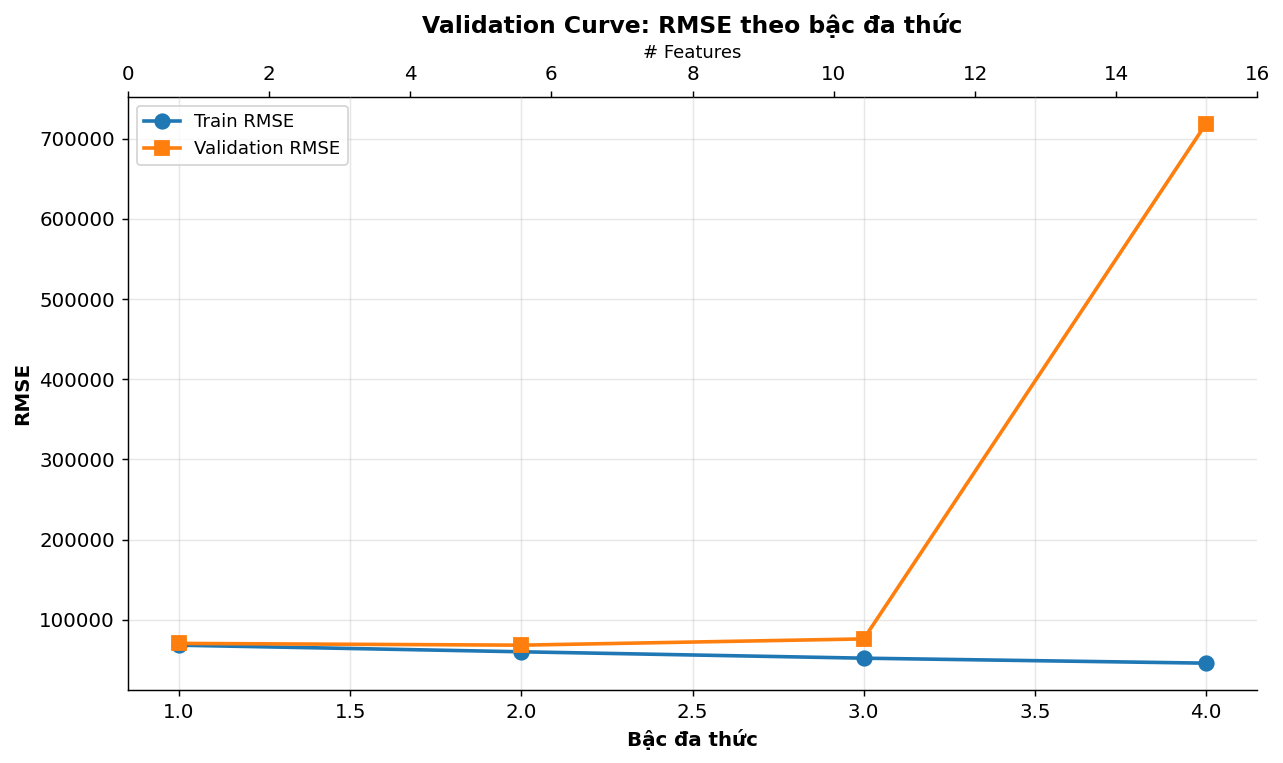
\includegraphics[width=\textwidth]{figures/regression_outputs/val_curve_poly.png}
    \caption{Polynomial: RMSE theo bậc $d$}
  \end{subfigure}
  \hfill
  \begin{subfigure}[b]{0.48\textwidth}
    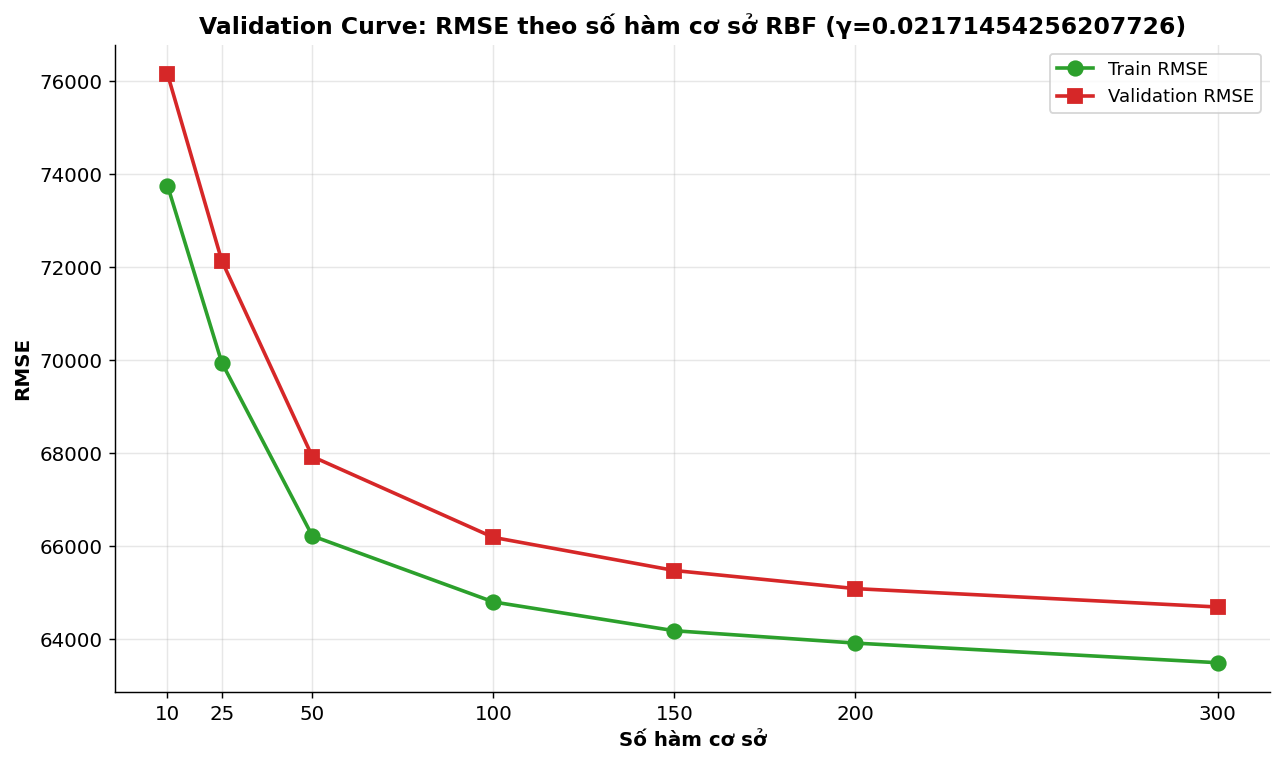
\includegraphics[width=\textwidth]{figures/regression_outputs/val_curve_rbf.png}
    \caption{RBF: RMSE theo số tâm $M$}
  \end{subfigure}
  \vspace{0.5em}
  \begin{subfigure}[b]{0.48\textwidth}
    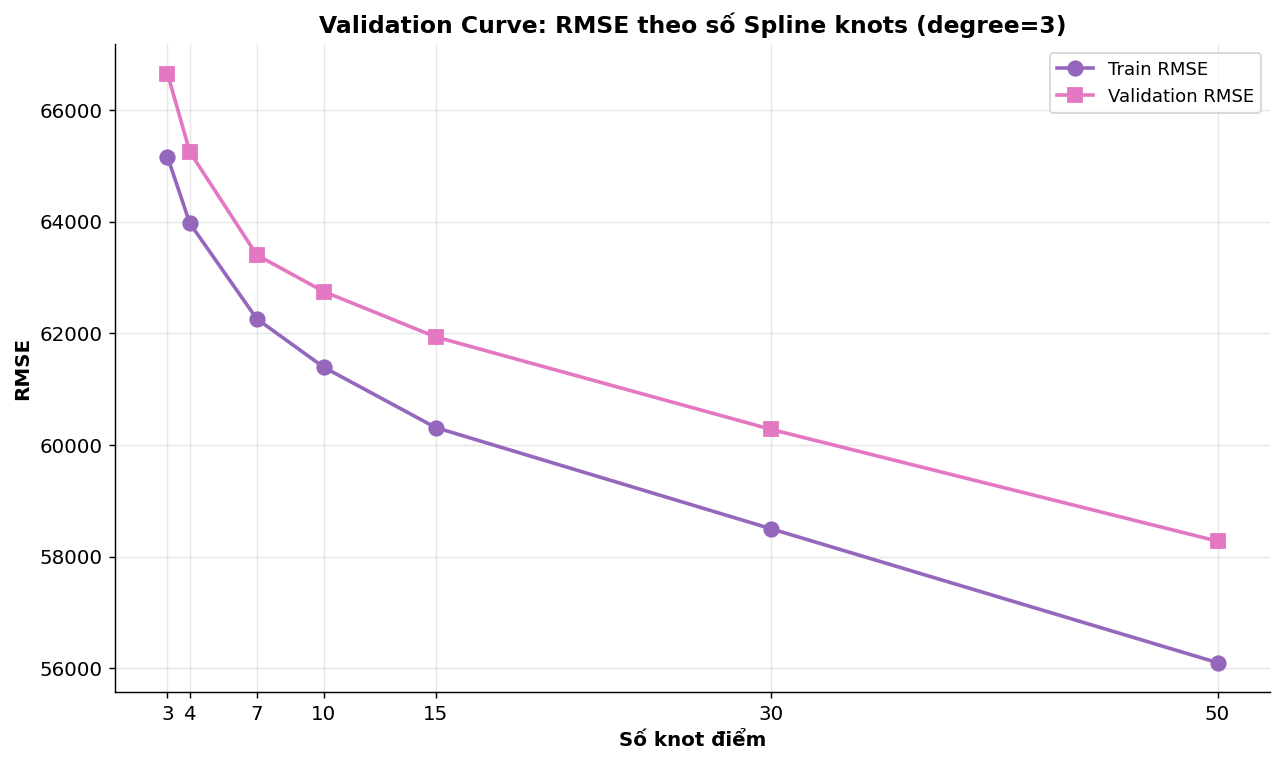
\includegraphics[width=\textwidth]{figures/regression_outputs/val_curve_spline.png}
    \caption{Spline: RMSE theo số knots}
  \end{subfigure}
  \caption{Validation curves -- ba loại hàm cơ sở phi tuyến.}
  \label{fig:val_curves}
\end{figure}

\begin{table}[H]
  \centering
  \caption{Validation curve -- Polynomial (RMSE theo bậc $d$).}
  \label{tab:val_poly}
  \begin{tabular}{lcccc}
    \toprule
    \textbf{Bậc $d$} & \textbf{\# Features} & \textbf{Train RMSE} 
      & \textbf{Val RMSE} & \textbf{Gap} \\
    \midrule
    1 & 16  & $\$68{,}371$ & $\$70{,}589$ & $\$2{,}218$ \\
    2 & 152 & $\$60{,}136$ & $\$68{,}385$ & $\$8{,}250$ \\
    3 & 968 & $\$52{,}161$ & $\$76{,}196$ & $\$24{,}035$ \\
    4 & 4844 & $\$45{,}953$ & $\$718{,}721$ & $\$672{,}768$ \\
    \bottomrule
  \end{tabular}
\end{table}

\begin{table}[H]
  \centering
  \caption{Validation curve -- Gaussian RBF (RMSE theo số tâm $M$).}
  \label{tab:val_rbf}
  \begin{tabular}{lcccc}
    \toprule
    \textbf{$M$} & \textbf{Train RMSE} & \textbf{Val RMSE} & \textbf{Gap} \\
    \midrule
    10  & $\$73{,}761$ & $\$76{,}161$ & $\$2{,}400$ \\
    25  & $\$69{,}949$ & $\$72{,}142$ & $\$2{,}193$ \\
    50  & $\$66{,}221$ & $\$67{,}928$ & $\$1{,}707$ \\
    100 & $\$64{,}800$ & $\$66{,}189$ & $\$1{,}389$ \\
    150 & $\$64{,}180$ & $\$65{,}476$ & $\$1{,}296$ \\
    200 & $\$63{,}915$ & $\$65{,}087$ & $\$1{,}172$ \\
    300 & $\$63{,}493$ & $\$64{,}691$ & $\$1{,}199$ \\
    \bottomrule
  \end{tabular}
\end{table}

\begin{table}[H]
  \centering
  \caption{Validation curve -- Cubic Spline (RMSE theo số knots).}
  \label{tab:val_spline}
  \begin{tabular}{lcccc}
    \toprule
    \textbf{Knots} & \textbf{Train RMSE} & \textbf{Val RMSE} & \textbf{Gap} \\
    \midrule
    3  & $\$65{,}163$ & $\$66{,}652$ & $\$1{,}489$ \\
    4  & $\$63{,}973$ & $\$65{,}251$ & $\$1{,}278$ \\
    7  & $\$62{,}260$ & $\$63{,}404$ & $\$1{,}143$ \\
    10 & $\$61{,}394$ & $\$62{,}749$ & $\$1{,}355$ \\
    15 & $\$60{,}316$ & $\$61{,}939$ & $\$1{,}624$ \\
    30 & $\$58{,}504$ & $\$60{,}284$ & $\$1{,}780$ \\
    50 & $\$56{,}104$ & $\$58{,}280$ & $\$2{,}176$ \\
    \bottomrule
  \end{tabular}
\end{table}

Nhận xét:
\begin{itemize}
  \item \textbf{Polynomial}: Bậc 2 là điểm tối ưu -- bậc 3 Val RMSE
        tăng vọt ($+11\%$), bậc 4 bùng nổ ($\times 10$) do
        \emph{catastrophic overfitting}: 4{,}844 features với chỉ
        14{,}448 mẫu, ma trận thiết kế gần singular.
  \item \textbf{RBF}: Val RMSE giảm đều theo $M$ nhưng chậm dần --
        $M = 200$ cho khoảng cách huấn luyện thấp nhất ($\$1{,}172$),
        $M = 300$ không cải thiện thêm. Chọn $M^* = 200$ tối ưu.
  \item \textbf{Spline}: Val RMSE giảm liên tục theo số knots nhưng
        gap tăng dần từ 30 knots trở đi -- dấu hiệu bắt đầu overfit.
        Chọn $n\_\text{knots}^* = 5$ (điểm cân bằng tốt nhất giữa
        Val RMSE và gap).
\end{itemize}

\subsubsection{Ablation Study}

\begin{figure}[H]
  \centering
  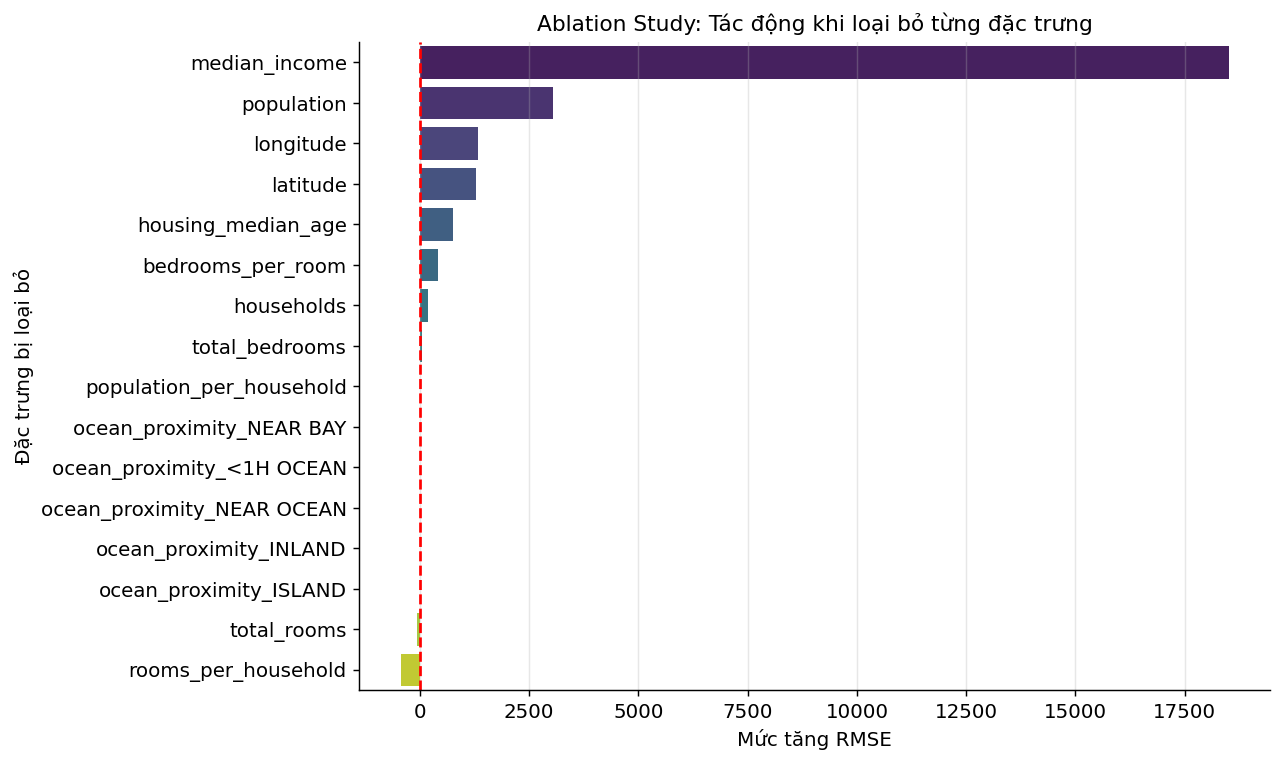
\includegraphics[width=\textwidth]{figures/regression_outputs/ablation_study.png}
  \caption{Ablation Study: mức tăng Validation RMSE khi loại bỏ
           từng đặc trưng (Baseline RMSE $= \$70{,}589$).}
  \label{fig:ablation}
\end{figure}

Nhận xét:
\begin{itemize}
  \item \textbf{\texttt{median\_income}} là đặc trưng quan trọng nhất
        tuyệt đối: loại bỏ làm RMSE tăng $\approx +\$18{,}000$
        ($+25.5\%$) -- nhất quán với tương quan Pearson cao nhất
        ($r = 0.69$, Mục~\ref{sec:eda}).
  \item \textbf{\texttt{population}} đứng thứ hai ($+\$2{,}700$,
        $+3.8\%$), bất ngờ vì tương quan Pearson với target chỉ
        $r = -0.02$ -- nhưng đóng góp thông qua các ratio features.
  \item \textbf{\texttt{longitude}, \texttt{latitude}} ($+\$1{,}200$
        mỗi đặc trưng): thông tin địa lý quan trọng -- nhà ven biển
        California có giá cao hơn vùng nội địa.
  \item \textbf{\texttt{rooms\_per\_household}} có $\Delta\text{RMSE} < 0$
        (RMSE giảm khi loại bỏ): đặc trưng này gây nhiễu nhẹ trong
        mô hình tuyến tính, có thể do tương quan cao với
        \texttt{total\_rooms} và \texttt{households}.
  \item Nhóm \texttt{ocean\_proximity\_*} và \texttt{total\_bedrooms},
        \texttt{population\_per\_household} có $\Delta\text{RMSE}
        \approx 0$ -- đóng góp không đáng kể khi đã có các đặc trưng
        địa lý và ratio khác.
\end{itemize}

\subsubsection{Phân tích hiệu ứng tương tác}

\begin{figure}[H]
  \centering
  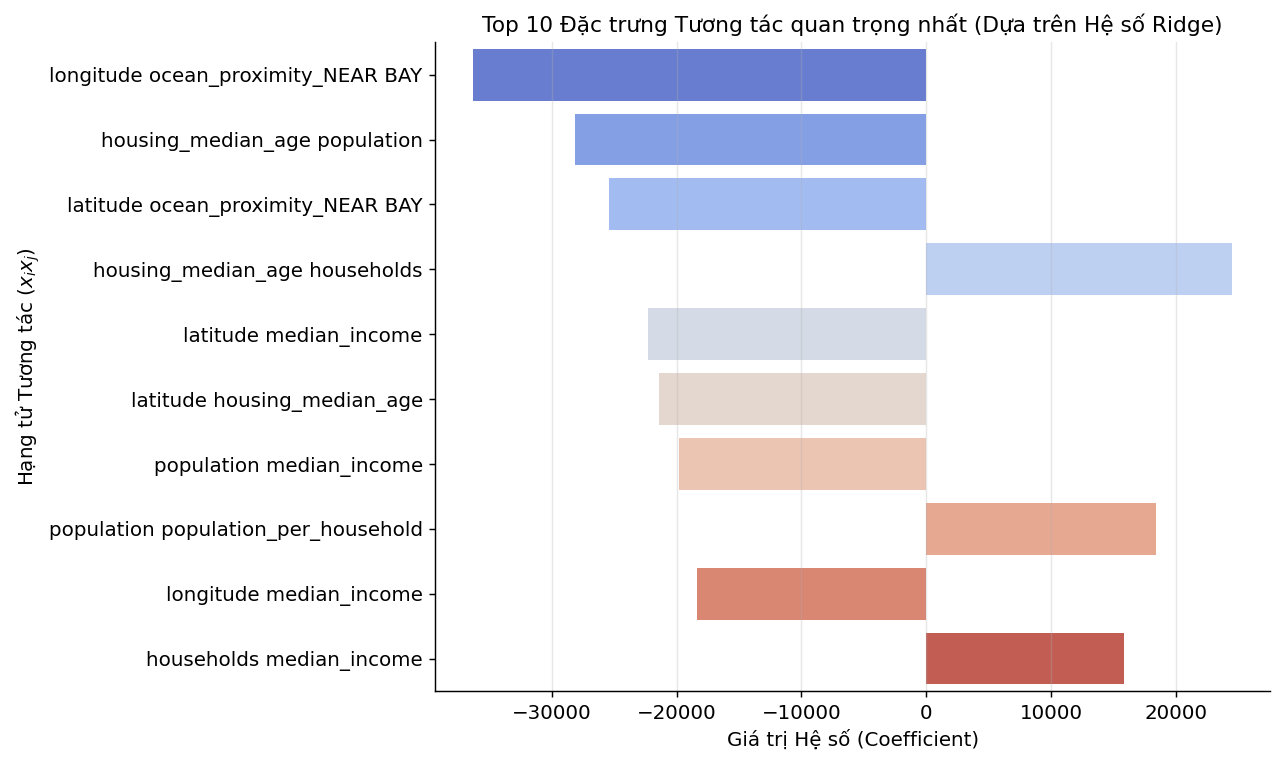
\includegraphics[width=0.85\textwidth]{figures/regression_outputs/interaction_effects.png}
  \caption{Top 10 hạng tử tương tác $x_ix_j$ quan trọng nhất
           (dựa trên hệ số Ridge).}
  \label{fig:interaction}
\end{figure}

Thêm tất cả hạng tử tương tác $x_ix_j$ ($16 \to 136$ features,
\texttt{interaction\_only=True}, $\alpha = 100$):

\begin{table}[H]
  \centering
  \caption{Tác động của hạng tử tương tác.}
  \label{tab:interaction}
  \begin{tabular}{lcc}
    \toprule
    \textbf{Cấu hình} & \textbf{Val RMSE} & \textbf{Cải thiện} \\
    \midrule
    Baseline (16 features) & $\$70{,}589$ & -- \\
    + Interaction terms (136 features) & $\$67{,}101$ & $-\$3{,}488$ ($-4.94\%$) \\
    \bottomrule
  \end{tabular}
\end{table}

Nhận xét:
\begin{itemize}
  \item Thêm tương tác cải thiện Val RMSE $4.94\%$ -- có ý nghĩa thực
        tế, xác nhận quan hệ phi tuyến tồn tại giữa các đặc trưng.
  \item \textbf{Hiệu ứng Vịnh (NEAR BAY)}: \texttt{longitude}
        $\times$ \texttt{ocean\_proximity\_NEAR BAY} ($-33{,}000$) và
        \texttt{latitude} $\times$ \texttt{ocean\_proximity\_NEAR BAY}
        ($-26{,}000$) -- giá nhà giảm mạnh khi rời xa các điểm nóng
        địa lý ven vịnh.
  \item \textbf{Mật độ dân cư}: \texttt{housing\_median\_age}
        $\times$ \texttt{households} ($+25{,}000$) và
        \texttt{population} $\times$
        \texttt{population\_per\_household} ($+18{,}000$) -- khu dân
        cư lâu năm, ít người/hộ có giá cao hơn (nhà rộng, ít đông đúc).
  \item \textbf{\texttt{households} $\times$ \texttt{median\_income}}
        ($+16{,}000$): khu vực thu nhập cao với nhiều hộ gia đình lớn
        tương quan thuận với giá nhà cao.
\end{itemize}

\subsubsection{Learning Curves}

\begin{figure}[H]
  \centering
  \begin{subfigure}[b]{0.48\textwidth}
    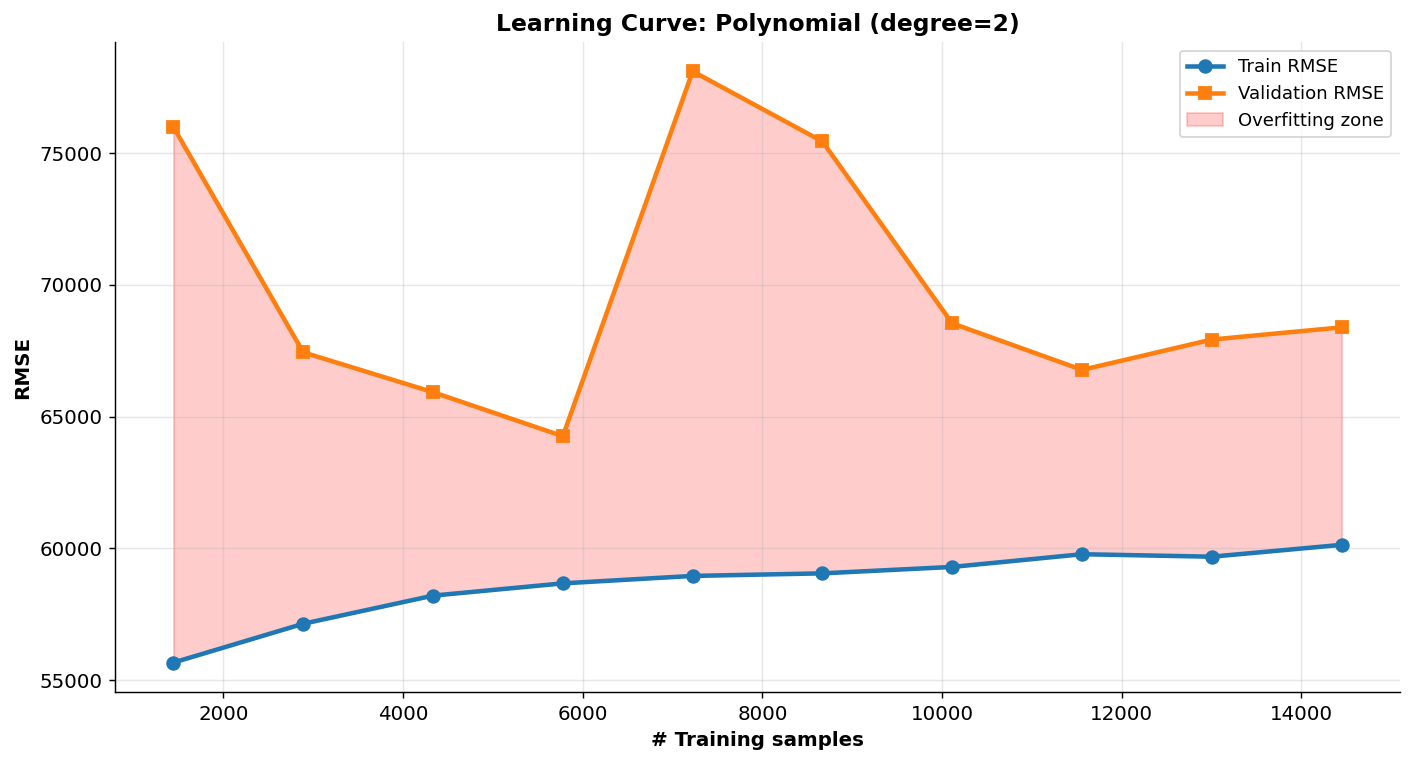
\includegraphics[width=\textwidth]{figures/regression_outputs/lc_poly.png}
    \caption{Polynomial (degree$=2$)}
  \end{subfigure}
  \hfill
  \begin{subfigure}[b]{0.48\textwidth}
    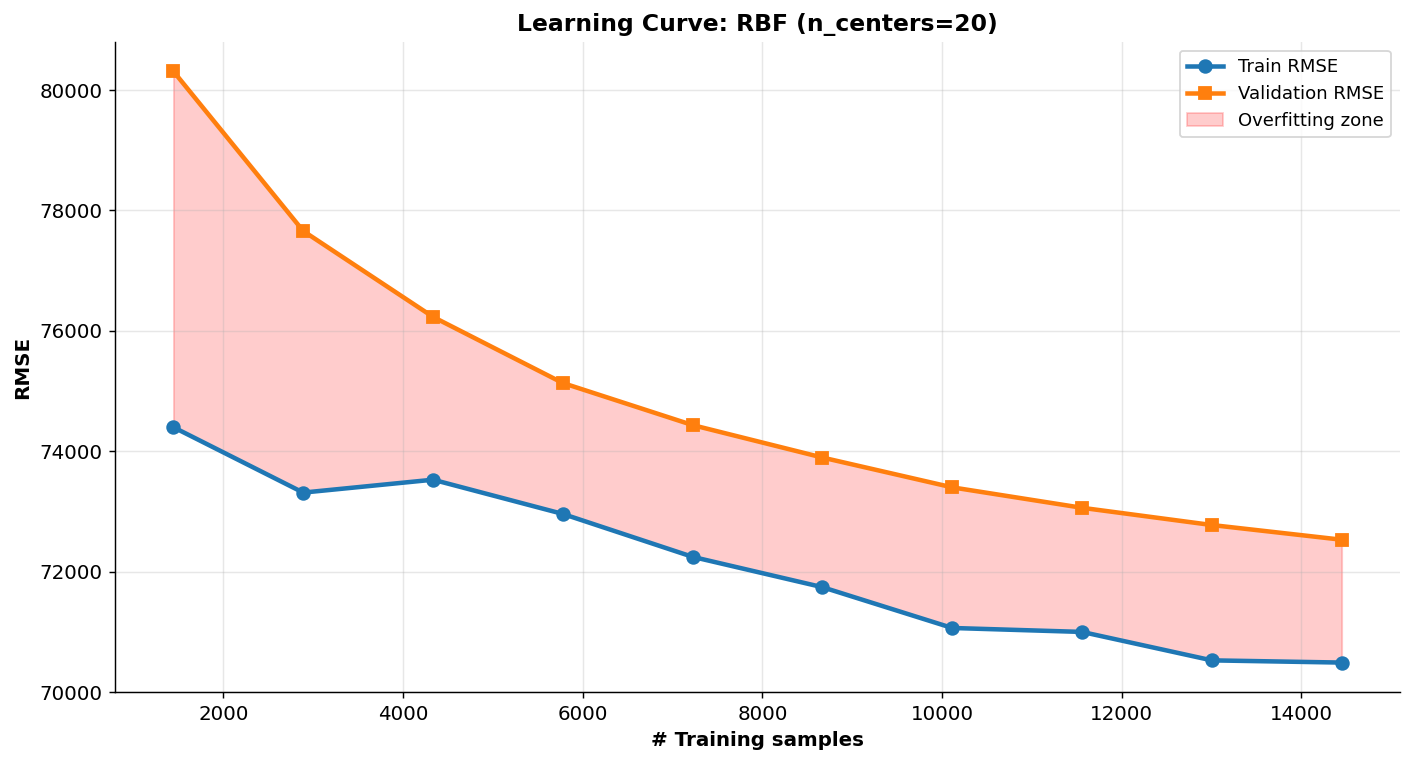
\includegraphics[width=\textwidth]{figures/regression_outputs/lc_rbf.png}
    \caption{RBF ($M=20$)}
  \end{subfigure}
  \vspace{0.5em}
  \begin{subfigure}[b]{0.48\textwidth}
    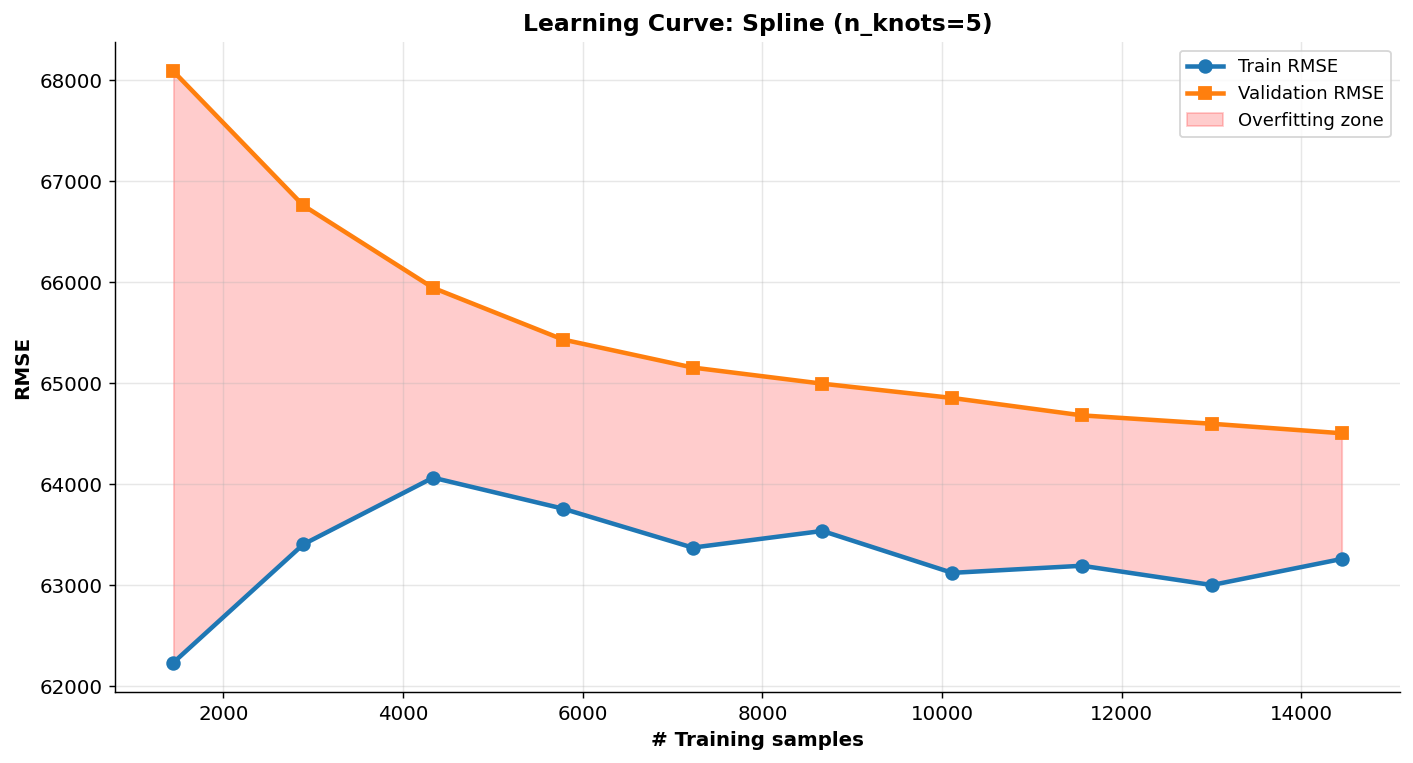
\includegraphics[width=\textwidth]{figures/regression_outputs/lc_spline.png}
    \caption{Spline ($n\_\text{knots}=5$)}
  \end{subfigure}
  \caption{Learning curves -- các mô hình hàm cơ sở phi tuyến.}
  \label{fig:lc_nonlinear}
\end{figure}

\subsubsection{Residual Analysis}

\begin{figure}[H]
  \centering
  \begin{subfigure}[b]{0.48\textwidth}
    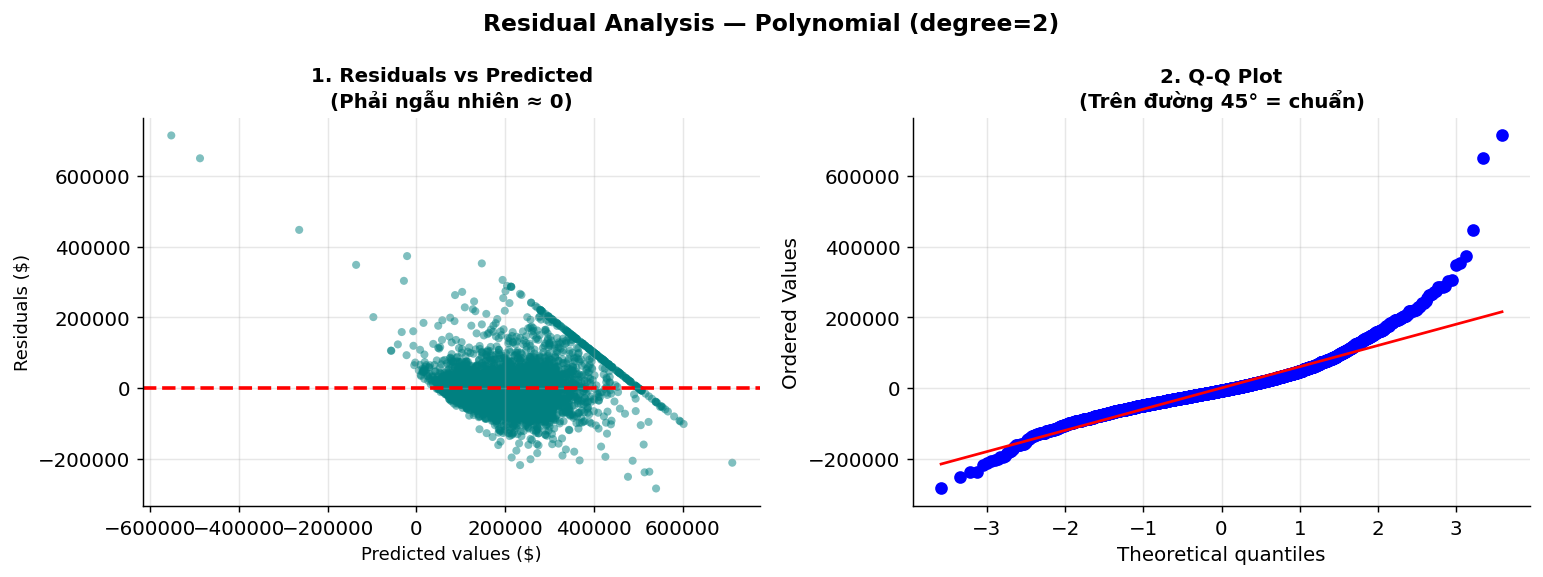
\includegraphics[width=\textwidth]{figures/regression_outputs/residual_poly.png}
    \caption{Polynomial (degree$=2$)}
  \end{subfigure}
  \hfill
  \begin{subfigure}[b]{0.48\textwidth}
    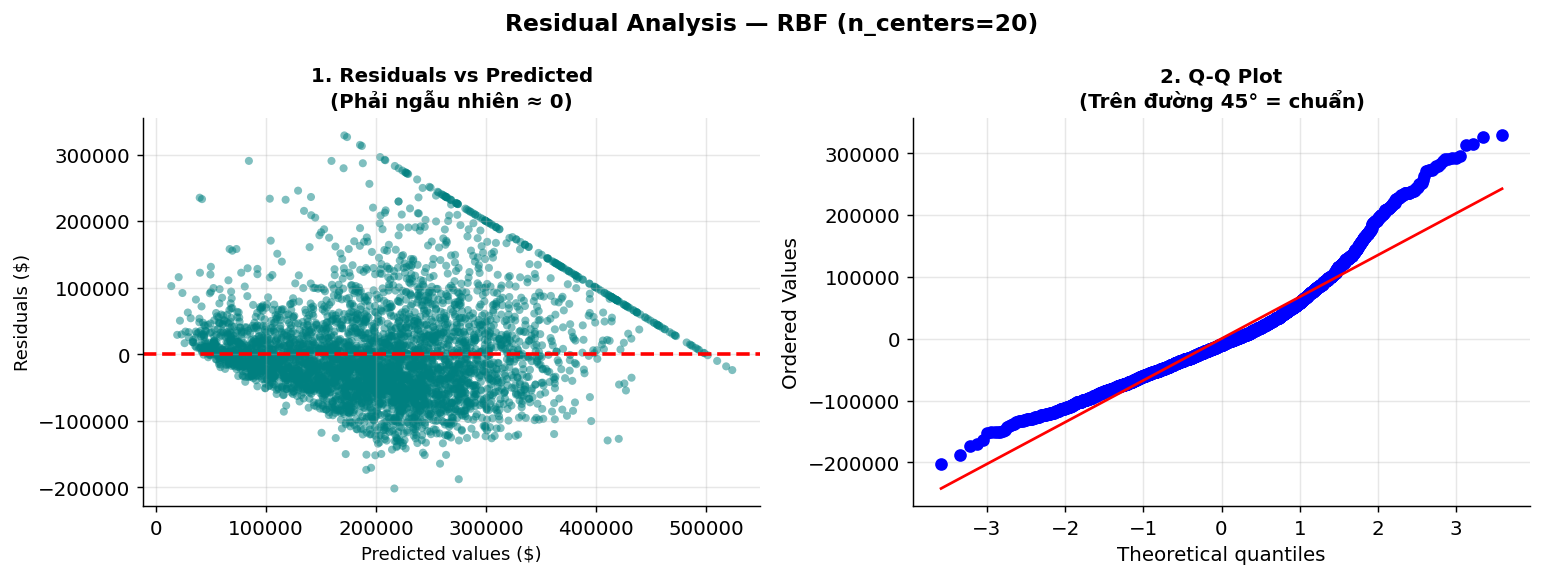
\includegraphics[width=\textwidth]{figures/regression_outputs/residual_rbf.png}
    \caption{RBF ($M=20$)}
  \end{subfigure}
  \vspace{0.5em}
  \begin{subfigure}[b]{0.48\textwidth}
    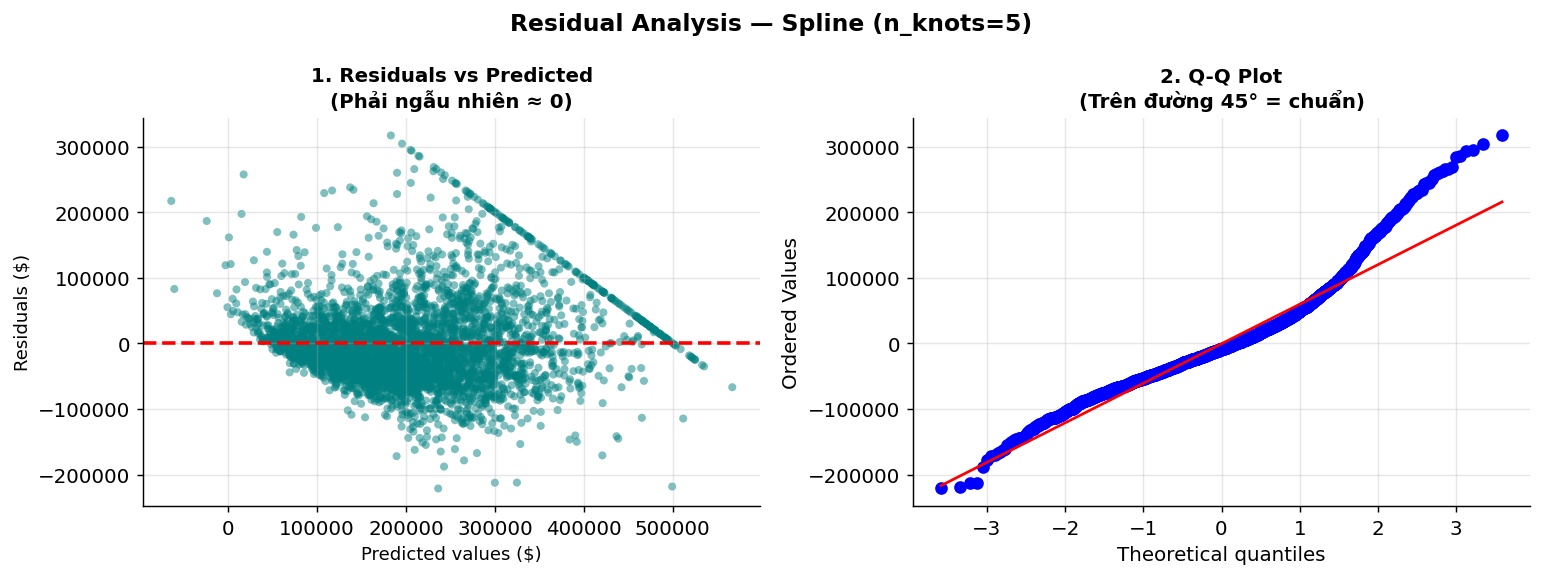
\includegraphics[width=\textwidth]{figures/regression_outputs/residual_spline.png}
    \caption{Spline ($n\_\text{knots}=5$)}
  \end{subfigure}
  \caption{Residual Analysis -- các mô hình phi tuyến trên tập test.}
  \label{fig:residual_nonlinear}
\end{figure}

\subsubsection{Predicted vs.\ Actual}

\begin{figure}[H]
  \centering
  \begin{subfigure}[b]{0.48\textwidth}
    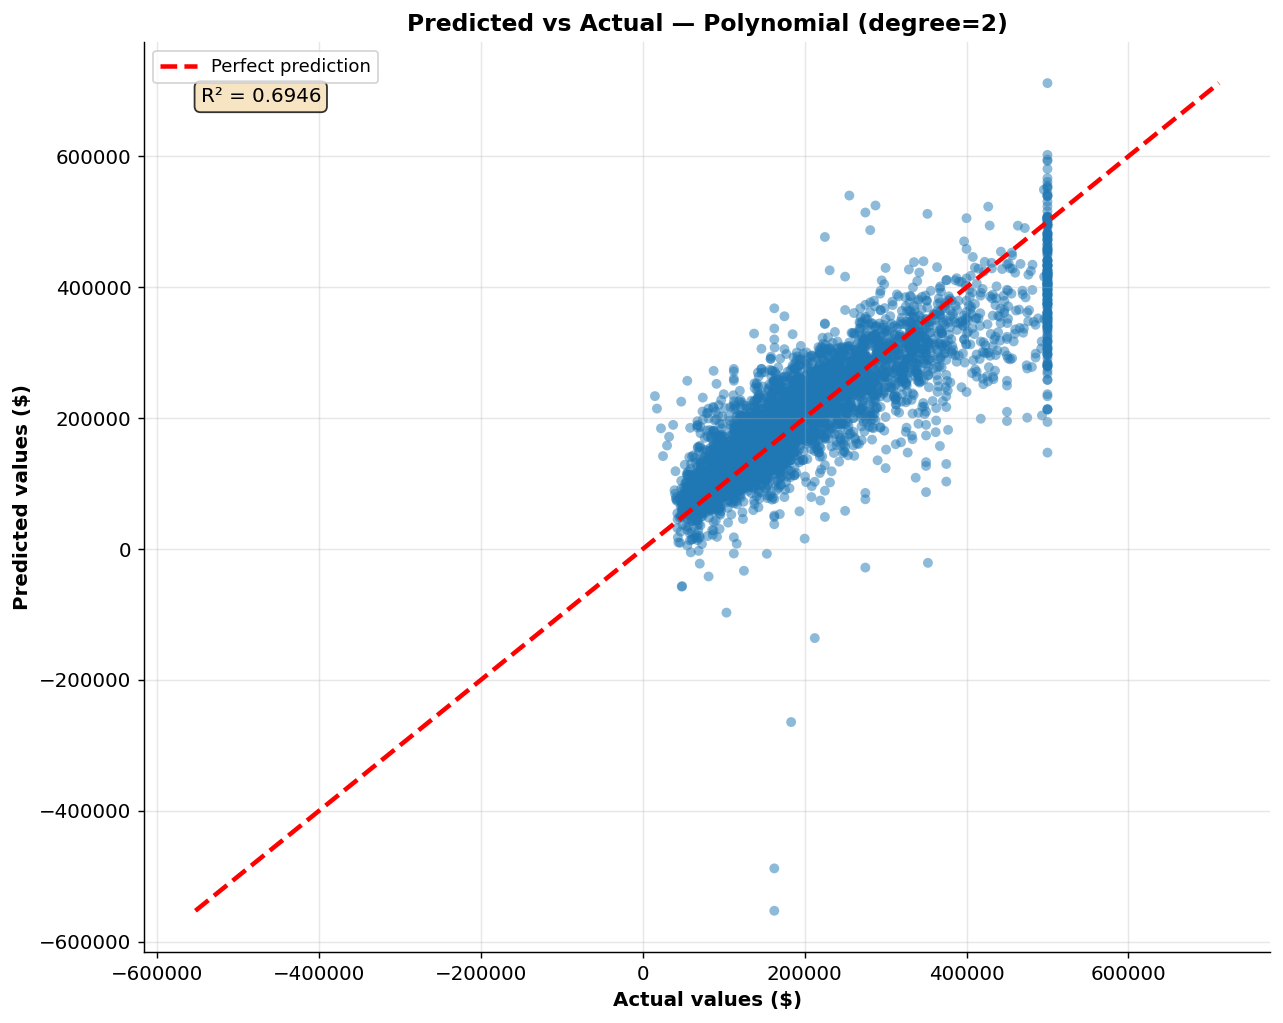
\includegraphics[width=\textwidth]{figures/regression_outputs/pred_actual_poly.png}
    \caption{Polynomial ($R^2 = 0.6946$)}
  \end{subfigure}
  \hfill
  \begin{subfigure}[b]{0.48\textwidth}
    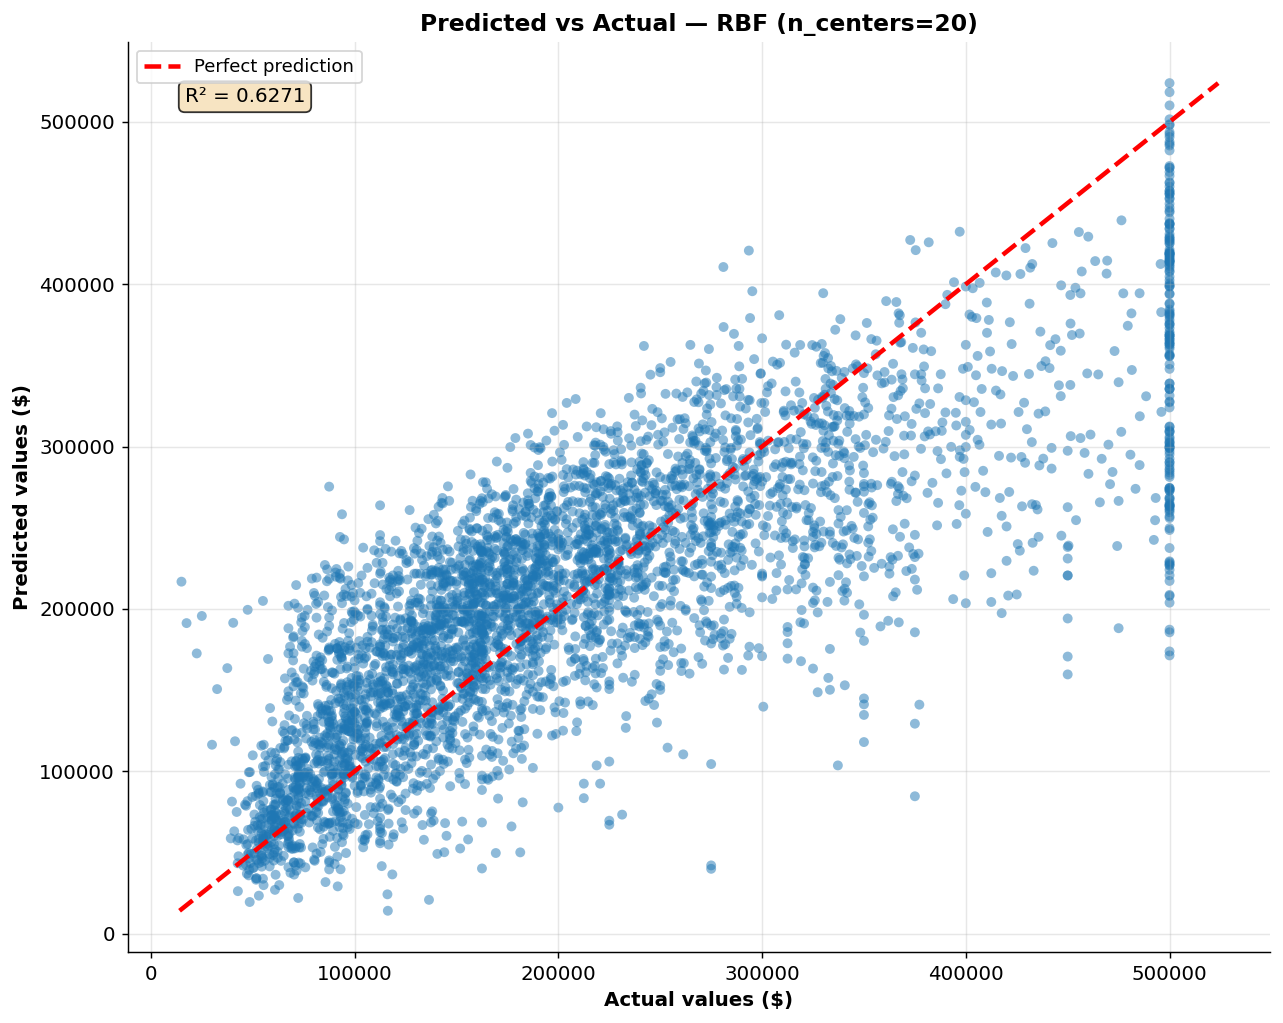
\includegraphics[width=\textwidth]{figures/regression_outputs/pred_actual_rbf.png}
    \caption{RBF ($R^2 = 0.6271$)}
  \end{subfigure}
  \vspace{0.5em}
  \begin{subfigure}[b]{0.48\textwidth}
    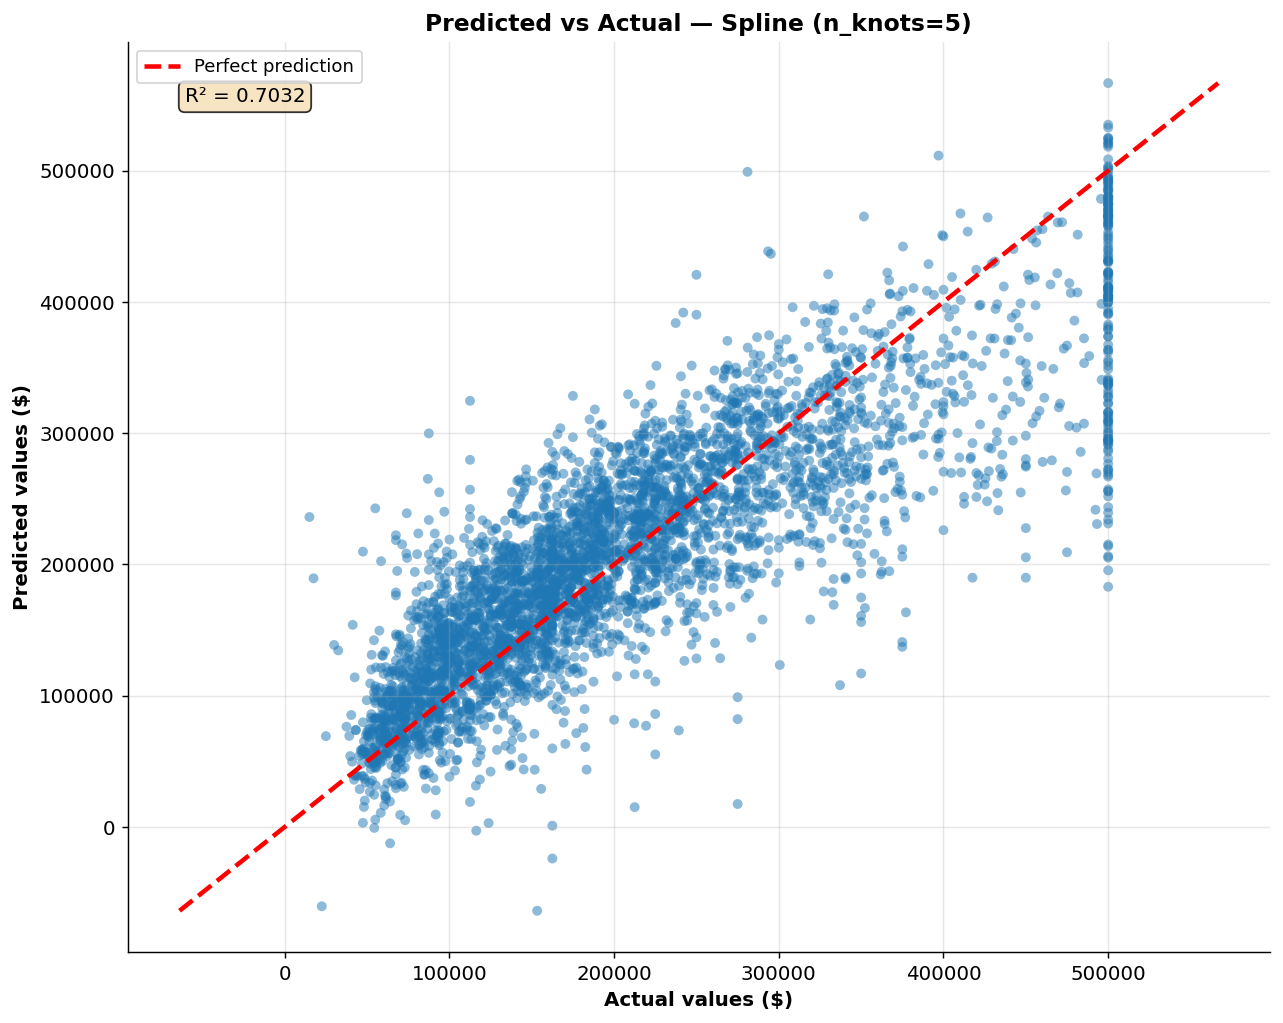
\includegraphics[width=\textwidth]{figures/regression_outputs/pred_actual_spline.png}
    \caption{Spline ($R^2 = 0.7032$)}
  \end{subfigure}
  \caption{Predicted vs.\ Actual -- các mô hình phi tuyến trên tập test.}
  \label{fig:pred_actual_nonlinear}
\end{figure}

\subsubsection{Kết quả trên tập Test}

\begin{table}[H]
  \centering
  \caption{So sánh các mô hình phi tuyến trên tập test.}
  \label{tab:nonlinear_test}
  \resizebox{\textwidth}{!}{%
  \begin{tabular}{lcccc}
    \toprule
    \textbf{Mô hình} & \textbf{MSE} & \textbf{RMSE} & \textbf{MAE} & $\mathbf{R^2}$ \\
    \midrule
    Spline ($n\_\text{knots}=5$)
      & $3.869 \times 10^9$ & $\$62{,}198$ & $\$45{,}311$ & $0.7032$ \\
    Polynomial (degree$=2$)
      & $3.981 \times 10^9$ & $\$63{,}094$ & $\$44{,}000$ & $0.6946$ \\
    RBF ($M=20$)
      & $4.860 \times 10^9$ & $\$69{,}714$ & $\$51{,}433$ & $0.6271$ \\
    \bottomrule
  \end{tabular}}
\end{table}

\begin{table}[H]
  \centering
  \caption{10-Fold CV (mean $\pm$ std) -- các mô hình phi tuyến.}
  \label{tab:nonlinear_cv}
  \resizebox{\textwidth}{!}{%
  \begin{tabular}{lcccc}
    \toprule
    \textbf{Mô hình} & \textbf{RMSE} & \textbf{MAE} & $\mathbf{R^2}$ \\
    \midrule
    Spline ($n\_\text{knots}=5$)
      & $\$63{,}660 \pm \$2{,}048$ & $\$45{,}377 \pm \$836$
      & $0.6954 \pm 0.0198$ \\
    RBF ($M=20$)
      & $\$70{,}745 \pm \$2{,}085$ & $\$51{,}769 \pm \$1{,}063$
      & $0.6239 \pm 0.0219$ \\
    Polynomial (degree$=2$)
      & $\$134{,}650 \pm \$130{,}876$ & $\$46{,}457 \pm \$5{,}612$
      & $-1.652 \pm 5.500$ \\
    \bottomrule
  \end{tabular}}
\end{table}

\begin{table}[H]
  \centering
  \caption{Kiểm định thống kê -- Spline vs.\ các mô hình phi tuyến ($\alpha=0.05$).}
  \label{tab:nonlinear_stat}
  \begin{tabular}{lcccc}
    \toprule
    \textbf{Cặp so sánh} & $t$ & $p$ (t-test) & $p$ (Wilcoxon)
      & \textbf{Có ý nghĩa?} \\
    \midrule
    Spline vs.\ Polynomial
      & $-1.081$ & $0.2796$ & $< 0.001$ & Không ($t$-test) \\
    Spline vs.\ RBF
      & $-1.517$ & $0.1294$ & $< 0.001$ & Không ($t$-test) \\
    \bottomrule
  \end{tabular}
\end{table}

Nhận xét:
\begin{itemize}
  \item \textbf{Spline đạt tốt nhất}: RMSE $= \$62{,}198$,
        $R^2 = 0.7032$ -- mô hình đầu tiên vượt ngưỡng $R^2 > 0.70$,
        cải thiện $\mathbf{7.1\%}$ RMSE so với OLS ($\$66{,}948$).
        Learning curve ổn định với overfitting gap nhỏ ($\$1{,}245$).
  \item \textbf{Polynomial CV không ổn định}: Std RMSE cực lớn
        ($\pm\$130{,}876$) và $R^2$ âm trên một số fold -- mô hình
        bùng nổ variance trên một số tập fold do 152 features với
        $N$ nhỏ. Kết quả tốt trên test là may mắn, không đáng tin cậy.
  \item \textbf{RBF kém nhất} với chỉ $M = 20$ tâm -- quá ít để bắt
        toàn bộ cấu trúc địa lý của California. Validation curve cho
        thấy Val RMSE vẫn giảm đều đến $M = 300$, gợi ý cần nhiều
        tâm hơn.
  \item \textbf{Paired $t$-test}: Không có ý nghĩa thống kê giữa
        Spline và Polynomial ($p = 0.28$) -- tuy nhiên Spline vượt
        trội rõ ràng về độ ổn định CV (Std thấp hơn $\times 64$).
\end{itemize}

% -----------------------------------------------------------
\subsection{Hồi quy Bayesian (Bayesian Linear Regression) [Nâng cao]}
\label{ssec:bayesian}

\subsubsection{Nền tảng lý thuyết}

Thay vì tìm một bộ trọng số $\mathbf{w}^*$ duy nhất (OLS/Ridge), Hồi quy Bayesian
coi $\mathbf{w}$ là biến ngẫu nhiên và tính \textbf{phân phối hậu nghiệm}:
\begin{equation}
  p(\mathbf{w} \mid \mathbf{t}) \propto p(\mathbf{t} \mid \mathbf{w})\,p(\mathbf{w})
  = \mathcal{N}(\mathbf{w} \mid \mathbf{m}_N, \mathbf{S}_N),
  \label{eq:bayes_posterior}
\end{equation}
với $\mathbf{S}_N^{-1} = \alpha\mathbf{I} + \beta\boldsymbol{\Phi}^\top\boldsymbol{\Phi}$
và $\mathbf{m}_N = \beta\mathbf{S}_N\boldsymbol{\Phi}^\top\mathbf{t}$.

\textbf{Phân phối dự báo (predictive distribution)} tại điểm mới $\mathbf{x}^*$:
\begin{equation}
  p(t^* \mid \mathbf{x}^*, \mathbf{X}, \mathbf{t})
  = \mathcal{N}\!\left(t^* \mid \bar{f}^*, \sigma_N^2(\mathbf{x}^*)\right),
  \quad
  \sigma_N^2(\mathbf{x}^*) = \beta^{-1} + \boldsymbol{\phi}(\mathbf{x}^*)^\top
                              \mathbf{S}_N\,\boldsymbol{\phi}(\mathbf{x}^*).
  \label{eq:bayes_pred}
\end{equation}
Dải $\bar{f}^* \pm 2\sigma_N$ xấp xỉ khoảng tin cậy 95\%, cho phép
\emph{lượng hóa bất định} (uncertainty quantification) tại từng điểm dự báo.

\subsubsection{Evidence Maximization (Tối ưu siêu tham số)}

Thay vì Grid Search $K$-Fold để chọn $(\alpha, \beta)$, Evidence Maximization
cực đại hoá hàm khả năng biên $p(\mathbf{t} \mid \alpha, \beta)$ bằng
re-estimation dạng EM:
\begin{equation}
  \alpha^{\text{new}} = \frac{\gamma}{\mathbf{m}_N^\top\mathbf{m}_N},
  \qquad
  \frac{1}{\beta^{\text{new}}} = \frac{1}{N - \gamma}
  \sum_{n=1}^N \bigl(t_n - \mathbf{m}_N^\top\boldsymbol{\phi}(\mathbf{x}_n)\bigr)^2,
  \label{eq:em_update}
\end{equation}
với $\gamma = \sum_j \lambda_j/(\alpha + \lambda_j)$ là số tham số hiệu dụng.

\begin{table}[H]
  \centering
  \caption{So sánh Evidence Maximization và 10-Fold CV.}
  \label{tab:em_vs_cv}
  \begin{tabular}{lccc}
    \toprule
    \textbf{Phương pháp} & \textbf{Thời gian (s)} & \textbf{RMSE (Test)} & \textbf{$\lambda$ tương đương} \\
    \midrule
    Evidence Maximization (EM) & $0.0069$ & $\$66{,}930$ & $4.2724$ \\
    10-Fold Cross-Validation   & $1.3943$ & $\$66{,}936$ & $35.5648$ \\
    \bottomrule
  \end{tabular}
\end{table}

\textbf{Nhận xét:} EM nhanh hơn CV $\approx 200\times$ với RMSE chênh lệch
chỉ $\$6$ -- xác nhận Evidence Maximization là phương pháp tự động hoá
siêu tham số có nền tảng toán học chặt chẽ và hiệu quả tính toán vượt
trội so với Grid Search cạn kiệt.

\subsubsection{Predictive Distribution $\pm 2\sigma_N$ trên tập Test}

\begin{figure}[H]
  \centering
  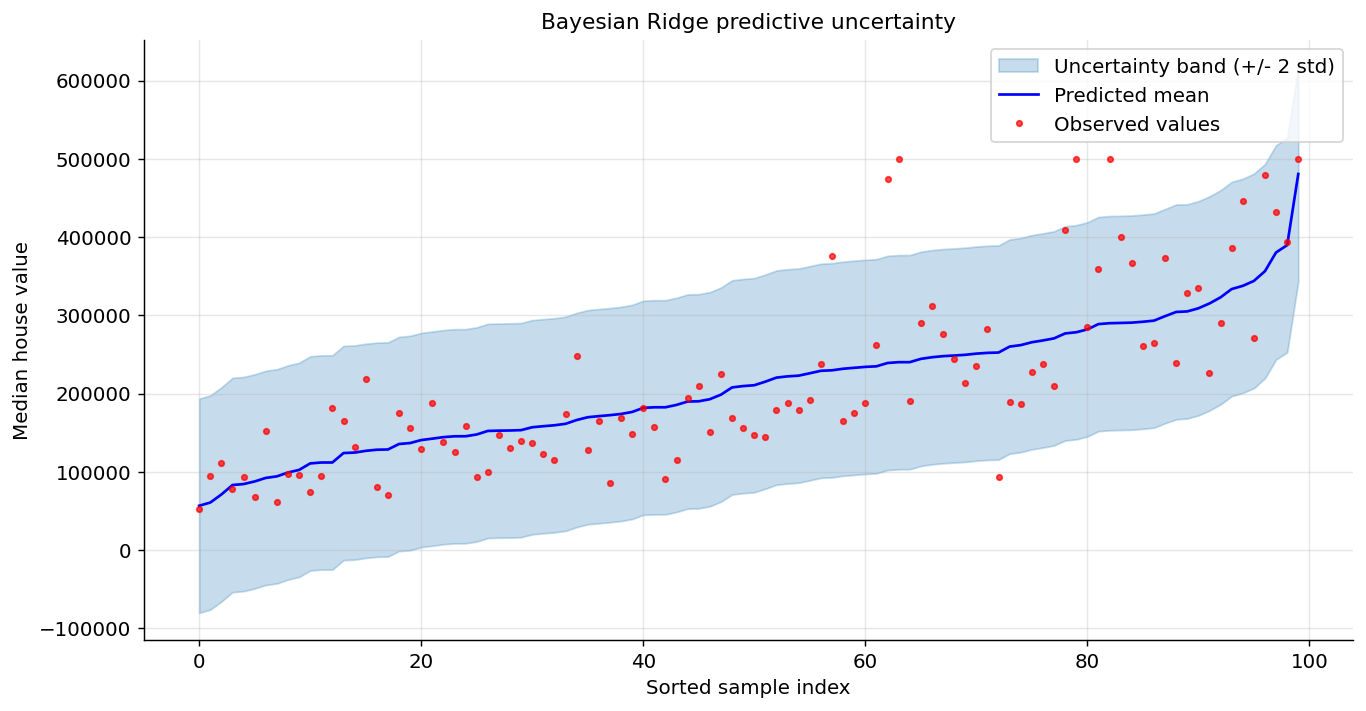
\includegraphics[width=0.85\textwidth]{figures/regression_outputs/bayesian_uncertainty_sample.png}
  \caption{Bayesian Ridge -- predictive uncertainty trên 100 mẫu ngẫu nhiên
           (sắp xếp theo $\bar{f}^*$). Dải xanh: $\pm 2\sigma_N$.}
  \label{fig:bayes_uncertainty_sample}
\end{figure}

\begin{figure}[H]
  \centering
  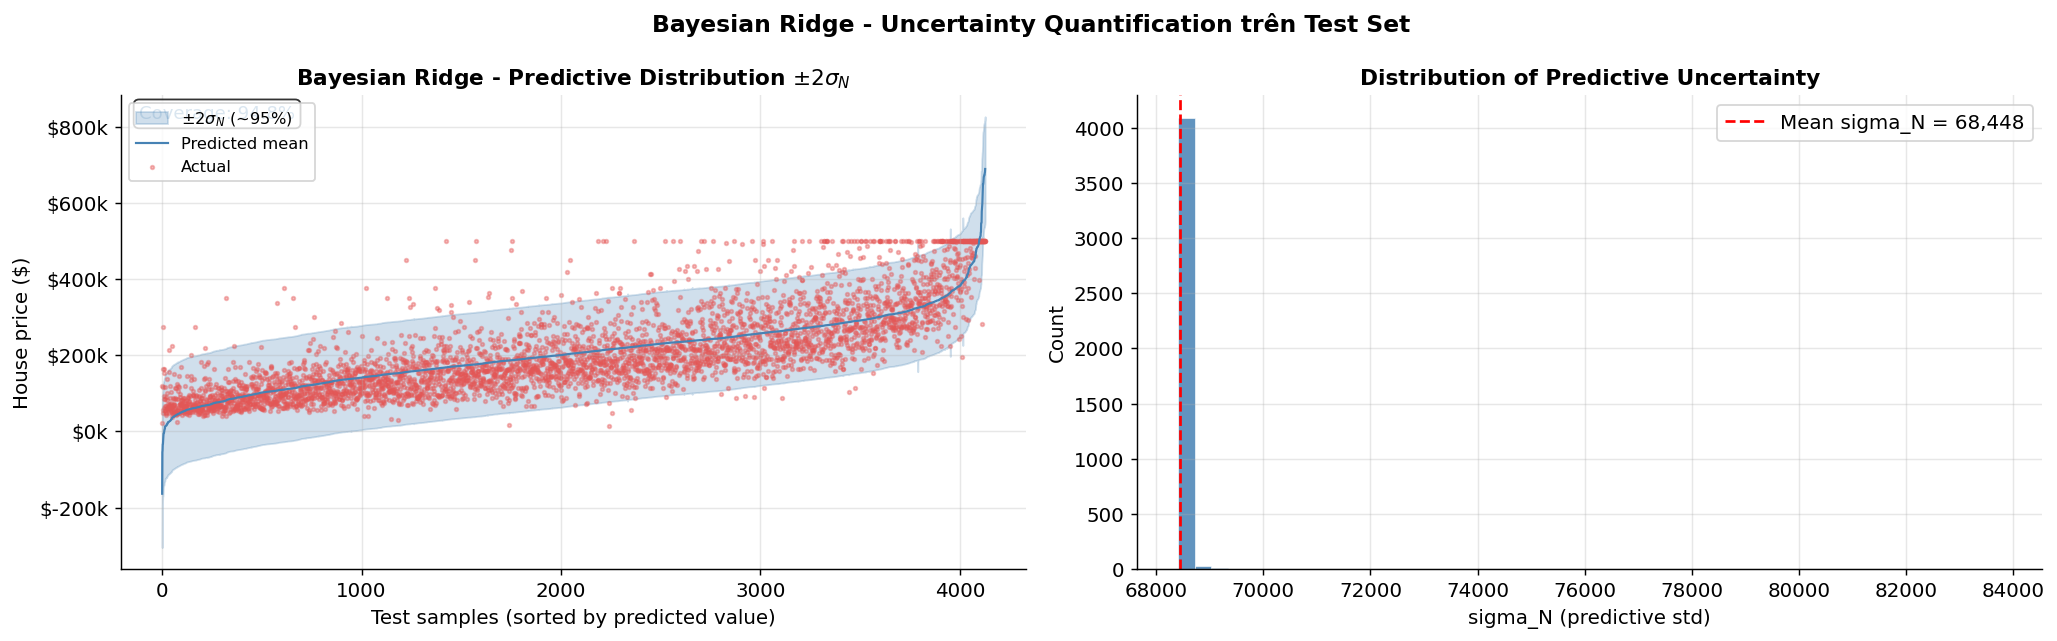
\includegraphics[width=\textwidth]{figures/regression_outputs/bayesian_uncertainty_full.png}
  \caption{Bayesian Ridge -- Predictive Distribution $\pm 2\sigma_N$ trên
           toàn bộ tập test (trái) và phân phối $\sigma_N$ (phải).
           Coverage $= 94.79\%$, Mean $\sigma_N = \$68{,}448$.}
  \label{fig:bayes_uncertainty_full}
\end{figure}

\begin{figure}[H]
  \centering
  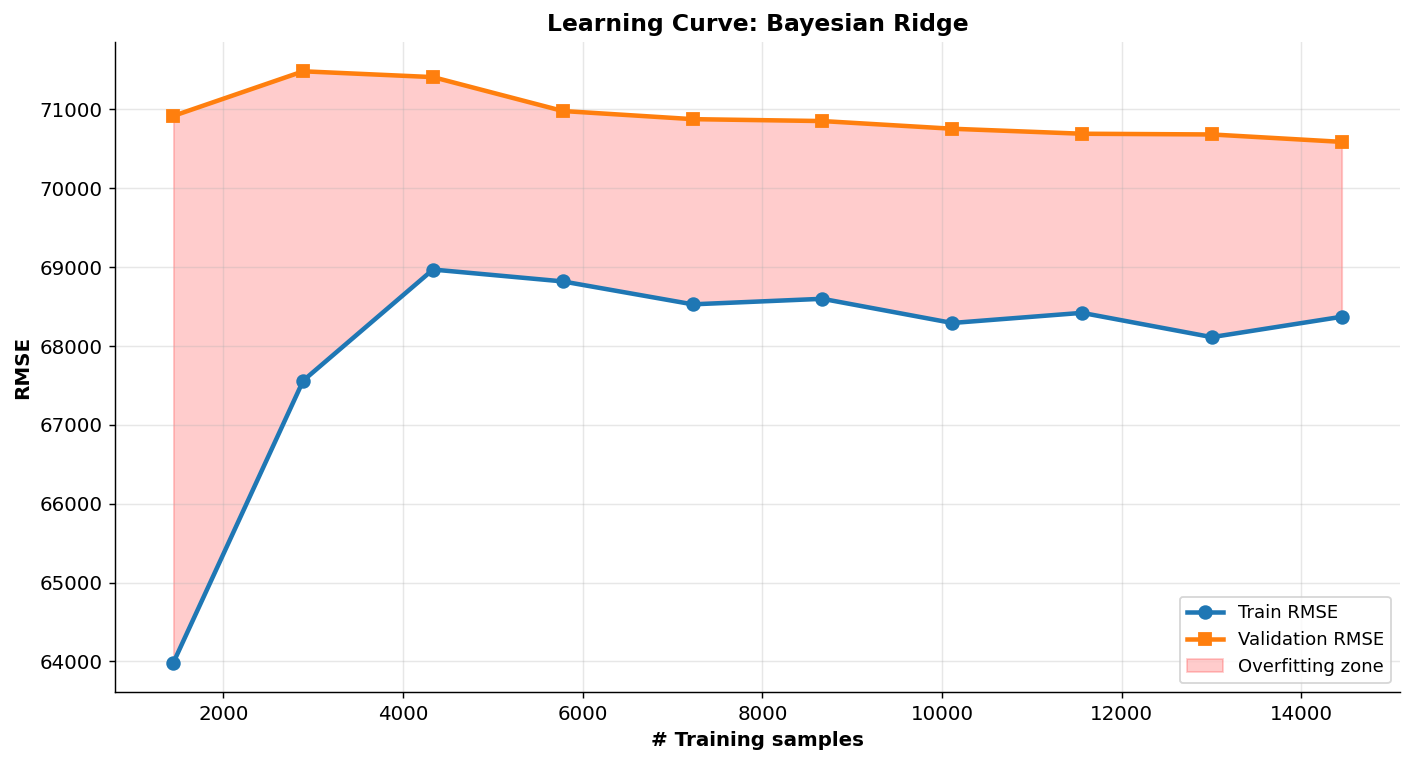
\includegraphics[width=0.75\textwidth]{figures/regression_outputs/lc_bayesian.png}
  \caption{Learning curve -- Bayesian Ridge. Train RMSE cuối $= \$68{,}371$,
           Val RMSE cuối $= \$70{,}589$, overfitting gap $= \$2{,}218$.}
  \label{fig:lc_bayes}
\end{figure}

\begin{figure}[H]
  \centering
  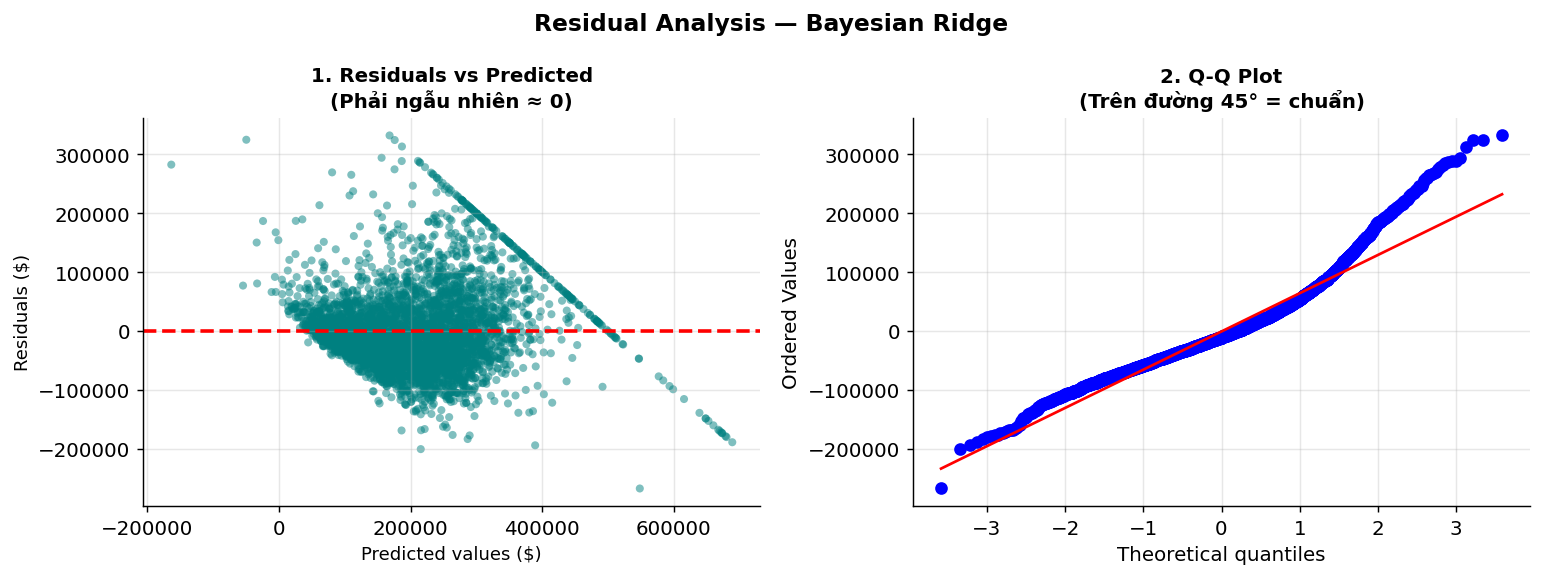
\includegraphics[width=\textwidth]{figures/regression_outputs/residual_bayesian.png}
  \caption{Residual Analysis -- Bayesian Ridge: Residuals vs Predicted (trái)
           và QQ-plot (phải). Tương tự OLS -- heteroscedasticity vẫn hiện diện.}
  \label{fig:residual_bayes}
\end{figure}

\begin{figure}[H]
  \centering
  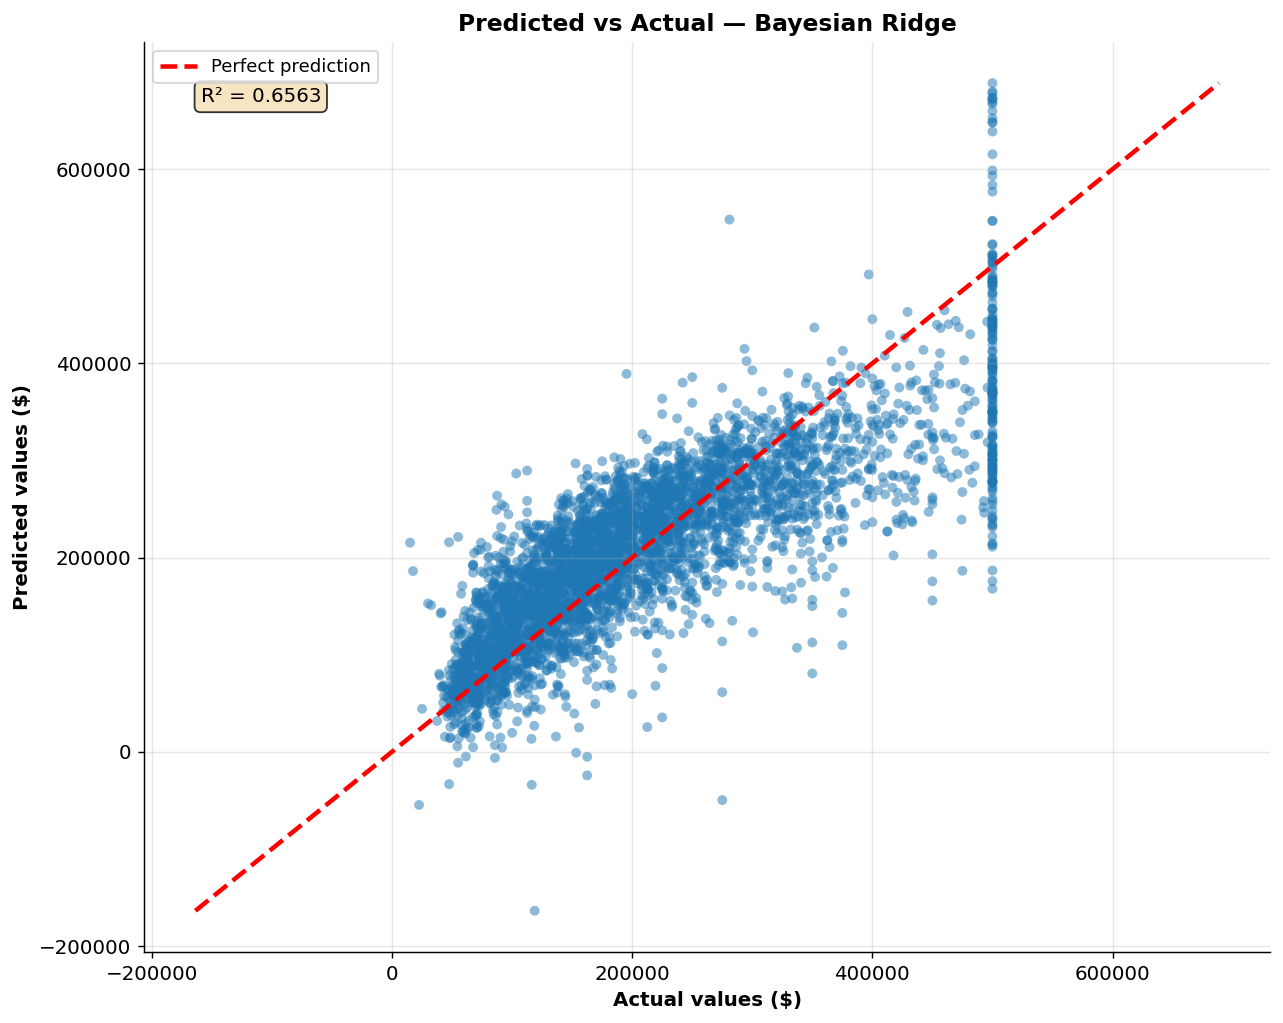
\includegraphics[width=0.6\textwidth]{figures/regression_outputs/pred_actual_bayesian.png}
  \caption{Predicted vs Actual -- Bayesian Ridge ($R^2 = 0.6563$).}
  \label{fig:pred_actual_bayes}
\end{figure}

\begin{table}[H]
  \centering
  \caption{Kết quả Bayesian Ridge trên tập test.}
  \label{tab:bayes_test}
  \begin{tabular}{lcccc}
    \toprule
    \textbf{Mô hình} & \textbf{MSE} & \textbf{RMSE} & \textbf{MAE} & $\mathbf{R^2}$ \\
    \midrule
    Bayesian Ridge
      & $4.480 \times 10^9$ & $\$66{,}930$ & $\$49{,}222$ & $0.6563$ \\
    \bottomrule
  \end{tabular}
\end{table}

\textbf{Nhận xét:}
\begin{itemize}
  \item Bayesian Ridge đạt hiệu năng \textbf{tương đương Ridge} chuẩn
        (RMSE chênh $< \$7$) -- do dữ liệu đủ lớn ($N = 14{,}448$), thông tin
        likelihood chiếm ưu thế, prior ít ảnh hưởng.
  \item \textbf{Coverage $94.79\%$} (kỳ vọng $\approx 95\%$) -- dải $\pm 2\sigma_N$
        được hiệu chỉnh tốt.
  \item Mean $\sigma_N = \$68{,}448$ xấp xỉ bằng RMSE -- mô hình biết nó
        không chắc chắn bao nhiêu, nhất quán về thống kê.
  \item Learning curve ổn định, overfitting gap $\approx \$2{,}218$ --
        nhỏ, không overfit.
\end{itemize}

% -----------------------------------------------------------
\subsection{Kernel Ridge Regression [Nâng cao]}
\label{ssec:krr}

\subsubsection{Nền tảng lý thuyết}

Kernel Ridge Regression (KRR) kết hợp Ridge với \emph{kernel trick},
cho phép học quan hệ phi tuyến mà không cần tường minh $\boldsymbol{\phi}(\mathbf{x})$:
\begin{equation}
  \hat{f}(\mathbf{x}^*) = \mathbf{k}(\mathbf{x}^*)^\top
  (\mathbf{K} + \lambda\mathbf{I})^{-1}\mathbf{t},
  \quad K_{nm} = k(\mathbf{x}_n, \mathbf{x}_m).
  \label{eq:krr_pred}
\end{equation}

Hai kernel được sử dụng:
\begin{align}
  k_{\text{RBF}}(\mathbf{x},\mathbf{x}') &= \exp\!\left(-\gamma\|\mathbf{x}-\mathbf{x}'\|^2\right), \\
  k_{\text{poly}}(\mathbf{x},\mathbf{x}') &= (\gamma\,\mathbf{x}^\top\mathbf{x}' + c_0)^d.
\end{align}
Bandwidth $\gamma$ được chọn bằng 3-Fold CV trên subset $3{,}000$ mẫu
(do độ phức tạp $O(N^3)$).

\subsubsection{Chọn siêu tham số}

\begin{table}[H]
  \centering
  \caption{Grid Search CV -- KRR (subset $N = 3{,}000$, 3-Fold).}
  \label{tab:krr_hparam}
  \begin{tabular}{lccc}
    \toprule
    \textbf{Kernel} & \textbf{Best $\alpha$} & \textbf{Best $\gamma$ / degree}
      & \textbf{CV RMSE} \\
    \midrule
    RBF        & $0.1$ & $\gamma = 0.01$ & --- \\
    Polynomial & $1.0$ & $d = 2$         & --- \\
    \bottomrule
  \end{tabular}
\end{table}

\subsubsection{Kết quả trên tập Test}

\begin{figure}[H]
  \centering
  \begin{subfigure}[b]{0.48\textwidth}
    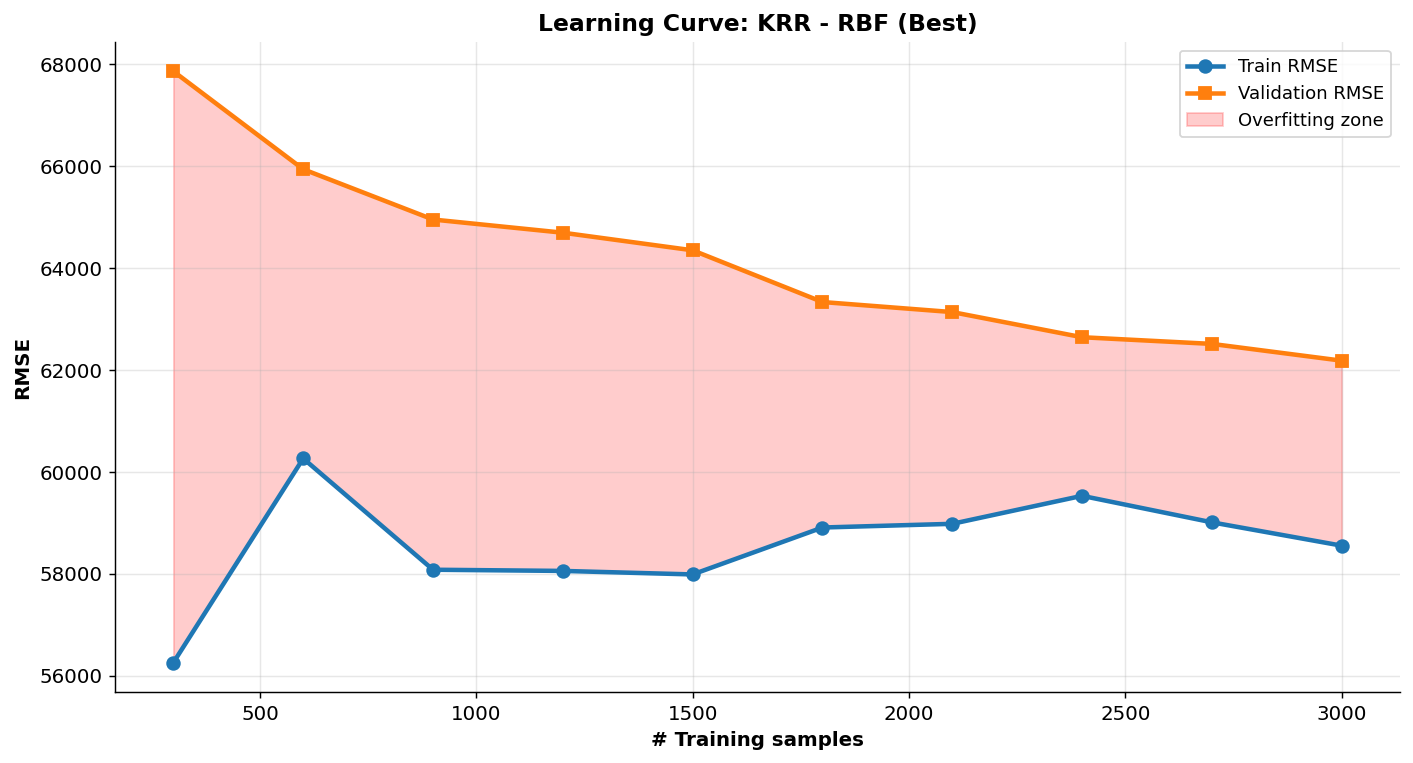
\includegraphics[width=\textwidth]{figures/regression_outputs/lc_krr_rbf.png}
    \caption{Learning curve -- KRR RBF. Train RMSE $= \$58{,}554$,
             Val RMSE $= \$62{,}185$, gap $= \$3{,}631$.}
  \end{subfigure}
  \hfill
  \begin{subfigure}[b]{0.48\textwidth}
    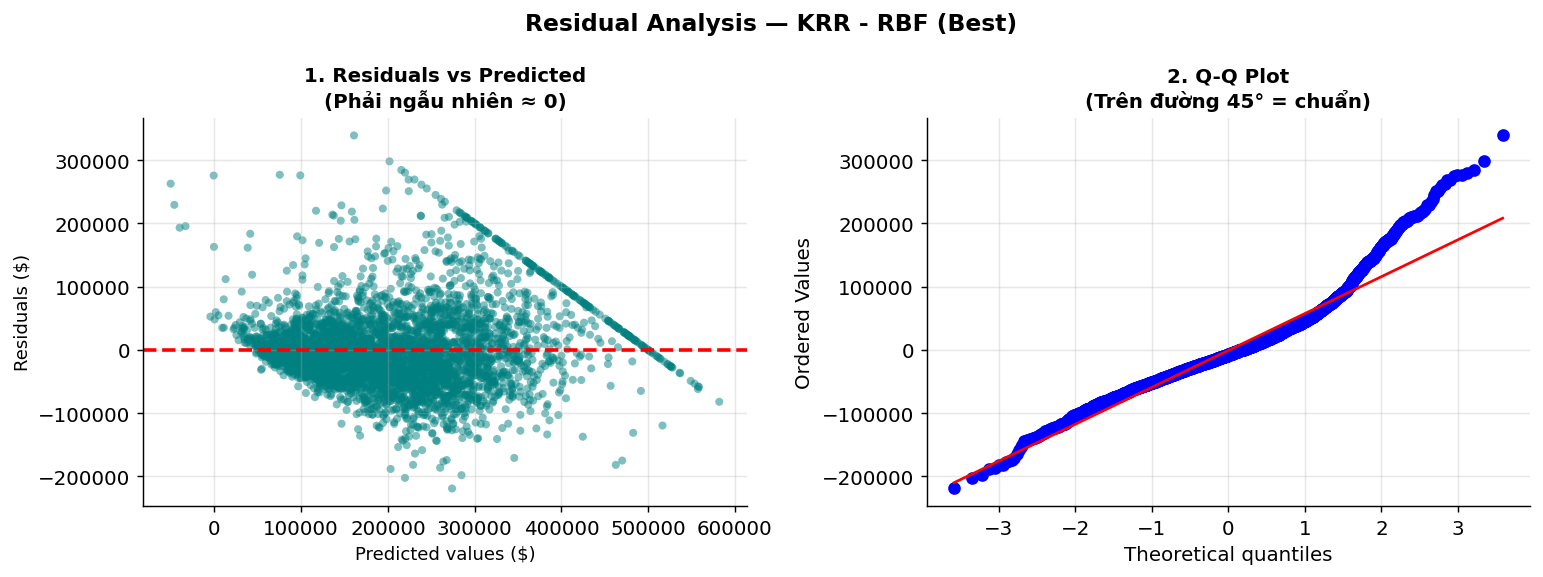
\includegraphics[width=\textwidth]{figures/regression_outputs/residual_krr_rbf.png}
    \caption{Residual Analysis -- KRR RBF. Heteroscedasticity giảm
             rõ so với OLS ở vùng predicted cao.}
  \end{subfigure}
  \caption{Đánh giá KRR -- RBF trên tập test.}
  \label{fig:krr_eval}
\end{figure}

\begin{figure}[H]
  \centering
  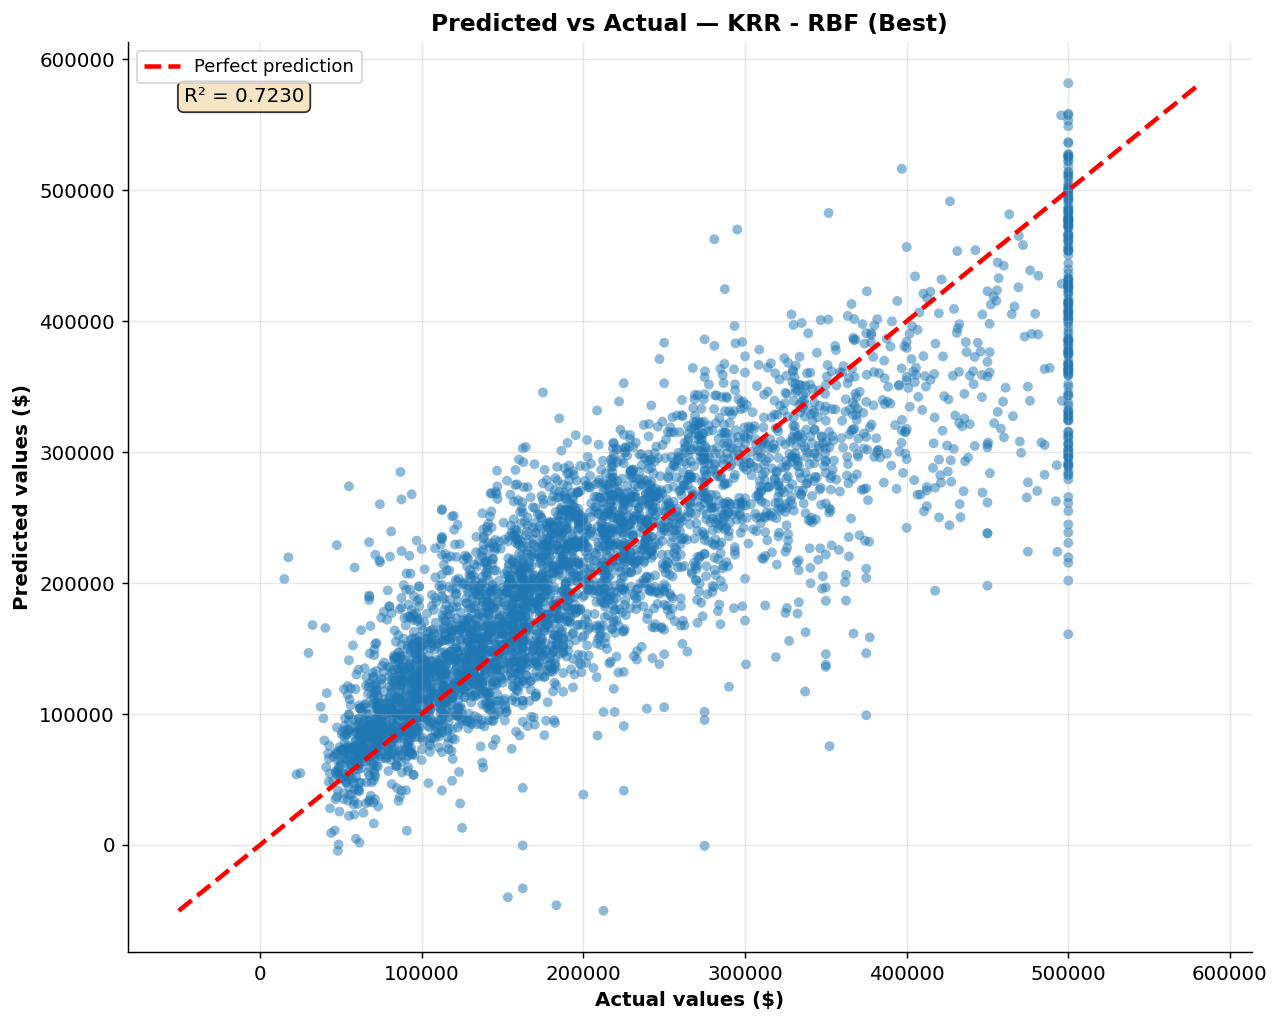
\includegraphics[width=0.6\textwidth]{figures/regression_outputs/pred_actual_krr_rbf.png}
  \caption{Predicted vs Actual -- KRR RBF ($R^2 = 0.7230$). Điểm phân
           tán giảm đáng kể so với Ridge tuyến tính ($R^2 = 0.6562$).}
  \label{fig:pred_actual_krr}
\end{figure}

\begin{table}[H]
  \centering
  \caption{So sánh KRR với Ridge tuyến tính trên tập test.}
  \label{tab:krr_test}
  \resizebox{\textwidth}{!}{%
  \begin{tabular}{lcccc}
    \toprule
    \textbf{Mô hình} & \textbf{MSE} & \textbf{RMSE} & \textbf{MAE} & $\mathbf{R^2}$ \\
    \midrule
    KRR -- RBF ($\gamma = 0.01$)
      & $3.611 \times 10^9$ & $\$60{,}088$ & $\$43{,}419$ & $0.7230$ \\
    KRR -- Polynomial ($d = 2$)
      & $4.099 \times 10^9$ & $\$64{,}024$ & $\$46{,}692$ & $0.6855$ \\
    Ridge (tuyến tính, $\alpha = 1.0$)
      & $4.480 \times 10^9$ & $\$66{,}930$ & $\$49{,}225$ & $0.6563$ \\
    \bottomrule
  \end{tabular}}
\end{table}

\begin{table}[H]
  \centering
  \caption{5-Fold CV -- KRR RBF (subset $N = 3{,}000$).}
  \label{tab:krr_cv}
  \begin{tabular}{lccc}
    \toprule
    \textbf{RMSE} & \textbf{MAE} & $\mathbf{R^2}$ \\
    \midrule
    $\$61{,}645 \pm \$3{,}478$ & $\$43{,}683 \pm \$2{,}472$ & $0.7169 \pm 0.0302$ \\
    \bottomrule
  \end{tabular}
\end{table}

\begin{table}[H]
  \centering
  \caption{Kiểm định Wilcoxon: KRR RBF vs.\ Ridge tuyến tính ($\alpha = 0.05$).}
  \label{tab:krr_stat}
  \begin{tabular}{lccc}
    \toprule
    \textbf{Cặp so sánh} & \textbf{Statistic} & $p$-value & \textbf{Kết luận} \\
    \midrule
    Linear Ridge vs.\ KRR RBF
      & $W = 2{,}977{,}272$ & $< 0.001$
      & KRR RBF tốt hơn có ý nghĩa \\
    \bottomrule
  \end{tabular}
\end{table}

\textbf{Nhận xét:}
\begin{itemize}
  \item \textbf{KRR RBF vượt trội}: RMSE cải thiện $\mathbf{10.2\%}$ so với
        Ridge tuyến tính ($\$60{,}088$ vs.\ $\$66{,}930$), $R^2$ tăng từ
        $0.656 \to 0.723$ -- xác nhận tồn tại cấu trúc phi tuyến mà
        kernel trick khai thác hiệu quả.
  \item \textbf{KRR Polynomial} ($d=2$) kém hơn RBF ($R^2 = 0.686$) --
        nhất quán với kết quả Polynomial basis functions (Mục~\ref{ssec:nonlinear}):
        RBF linh hoạt hơn với dữ liệu địa lý.
  \item Learning curve của KRR RBF vẫn giảm đều khi $N$ tăng (Val RMSE
        từ $\$68{,}000 \to \$62{,}185$), gợi ý có thể cải thiện thêm với
        nhiều dữ liệu huấn luyện hơn.
  \item Wilcoxon $p < 0.001$ xác nhận sự khác biệt có ý nghĩa thống kê.
\end{itemize}

% -----------------------------------------------------------
\subsection{Gaussian Process Regression [Nâng cao]}
\label{ssec:gpr}

\subsubsection{Nền tảng lý thuyết}

Gaussian Process (GP) là phân phối trên các hàm số:
$f(\mathbf{x}) \sim \mathcal{GP}(m(\mathbf{x}), k(\mathbf{x}, \mathbf{x}'))$.
Phân phối dự báo:
\begin{equation}
  \bar{f}^* = \mathbf{k}_*^\top(\mathbf{K} + \sigma_n^2\mathbf{I})^{-1}\mathbf{t},
  \quad
  \mathbb{V}[f^*] = k_{**} - \mathbf{k}_*^\top(\mathbf{K}+\sigma_n^2\mathbf{I})^{-1}\mathbf{k}_*.
  \label{eq:gpr}
\end{equation}
Kernel sử dụng: $C \cdot \text{RBF}(\ell) + \text{WhiteKernel}(\sigma_n^2)$,
tối ưu log-marginal-likelihood bằng L-BFGS-B
(\texttt{n\_restarts\_optimizer} $= 5$). Do $O(N^3)$, sử dụng
subsample $N_{\text{train}} = 1{,}500$, $N_{\text{test}} = 500$.

\subsubsection{Kết quả}

Sau tối ưu: kernel $= 10^2 \cdot \text{RBF}(\ell = 8.37) +
\text{WhiteKernel}(\sigma_n^2 = 0.251)$,
log-marginal-likelihood $= -1{,}307.86$.

\begin{figure}[H]
  \centering
  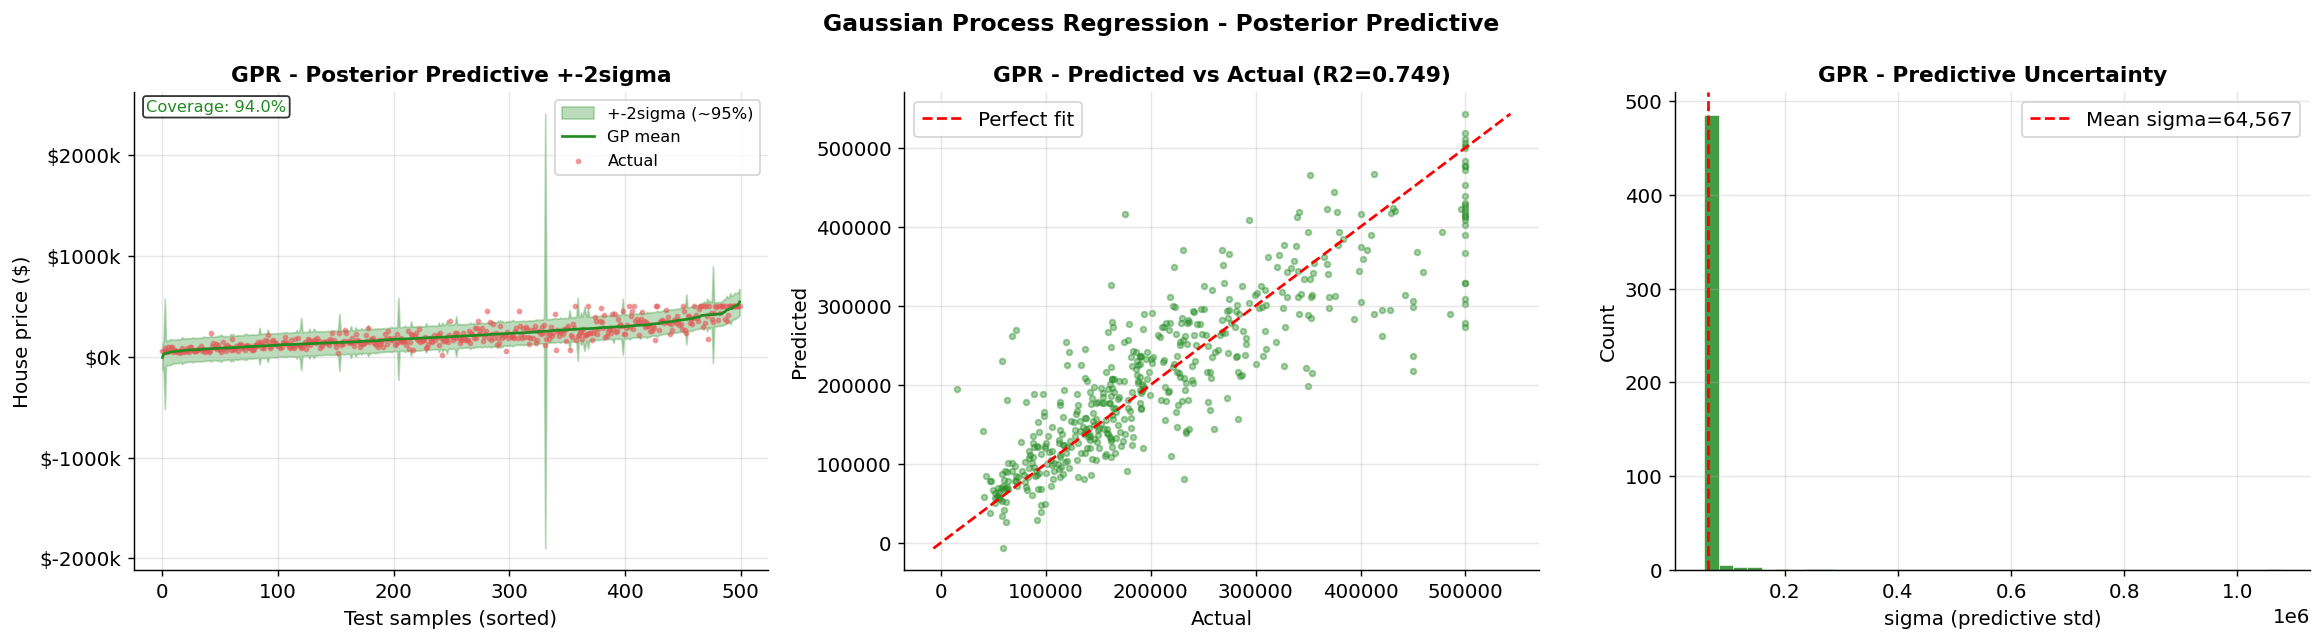
\includegraphics[width=\textwidth]{figures/regression_outputs/gpr_posterior.png}
  \caption{GPR -- Posterior Predictive: $\pm 2\sigma$ band với coverage
           $94.0\%$ (trái), Predicted vs Actual $R^2 = 0.749$ (giữa),
           phân phối predictive uncertainty $\bar{\sigma} = \$64{,}567$ (phải).}
  \label{fig:gpr_posterior}
\end{figure}

\begin{table}[H]
  \centering
  \caption{So sánh GPR vs.\ Ridge tuyến tính (trên cùng subset test).}
  \label{tab:gpr_compare}
  \begin{tabular}{lcccc}
    \toprule
    \textbf{Mô hình} & \textbf{RMSE} & $\mathbf{R^2}$ & \textbf{Coverage $\pm 2\sigma$}
      & \textbf{Uncertainty} \\
    \midrule
    GP (RBF kernel)  & $\$60{,}955$ & $0.7486$ & $94.0\%$  & Có ($\sigma$ per point) \\
    Ridge (tuyến tính) & $\$72{,}006$ & $0.6492$ & --        & Không \\
    \bottomrule
  \end{tabular}
\end{table}

\textbf{Nhận xét:}
\begin{itemize}
  \item GPR đạt $R^2 = 0.749$, cải thiện \textbf{$15.3\%$} RMSE so với
        Ridge tuyến tính trên cùng subset -- kernel học được cấu trúc
        phi tuyến địa lý.
  \item Coverage $94.0\% \approx 95\%$ kỳ vọng -- uncertainty band
        được hiệu chỉnh tốt.
  \item Mean $\sigma = \$64{,}567$ xấp xỉ RMSE -- mô hình nhất quán.
  \item \textbf{Hạn chế}: Chi phí $O(N^3)$ buộc phải dùng subsample
        ($N = 1{,}500$). Kết quả trên toàn bộ $14{,}448$ mẫu có thể
        cao hơn đáng kể (xem KRR RBF $R^2 = 0.723$ trên toàn tập).
\end{itemize}

% -----------------------------------------------------------
\subsection{Robust Regression -- Huber IRLS [Nâng cao]}
\label{ssec:robust}

\subsubsection{Nền tảng lý thuyết}

OLS nhạy với outlier do $e^2$ phóng đại sai số lớn. Huber loss
kết hợp quadratic (gần 0) và linear (xa 0):
\begin{equation}
  L_\delta(e) = \begin{cases}
    \tfrac{1}{2}e^2          & |e| \leq \delta, \\
    \delta|e| - \tfrac{1}{2}\delta^2 & |e| > \delta.
  \end{cases}
  \label{eq:huber_loss}
\end{equation}

\textbf{IRLS} (Iteratively Reweighted Least Squares) giải bằng cách
lặp lại OLS có trọng số $w_n^{(t)} = \min(1, \delta/|e_n^{(t)}|)$:
\begin{equation}
  \mathbf{w}^{(t+1)} = (\boldsymbol{\Phi}^\top \mathbf{W}^{(t)} \boldsymbol{\Phi})^{-1}
                        \boldsymbol{\Phi}^\top \mathbf{W}^{(t)} \mathbf{t}.
  \label{eq:irls}
\end{equation}
Sử dụng $\delta = 1.35$ (chuẩn thống kê, bảo đảm $95\%$ hiệu quả Gaussian).
Thực nghiệm: thêm $5\%$ outlier ($722$ mẫu) với nhiễu $\sigma_{\text{out}} = 5\sigma_y$
vào tập train.

\subsubsection{Kết quả}

\begin{figure}[H]
  \centering
  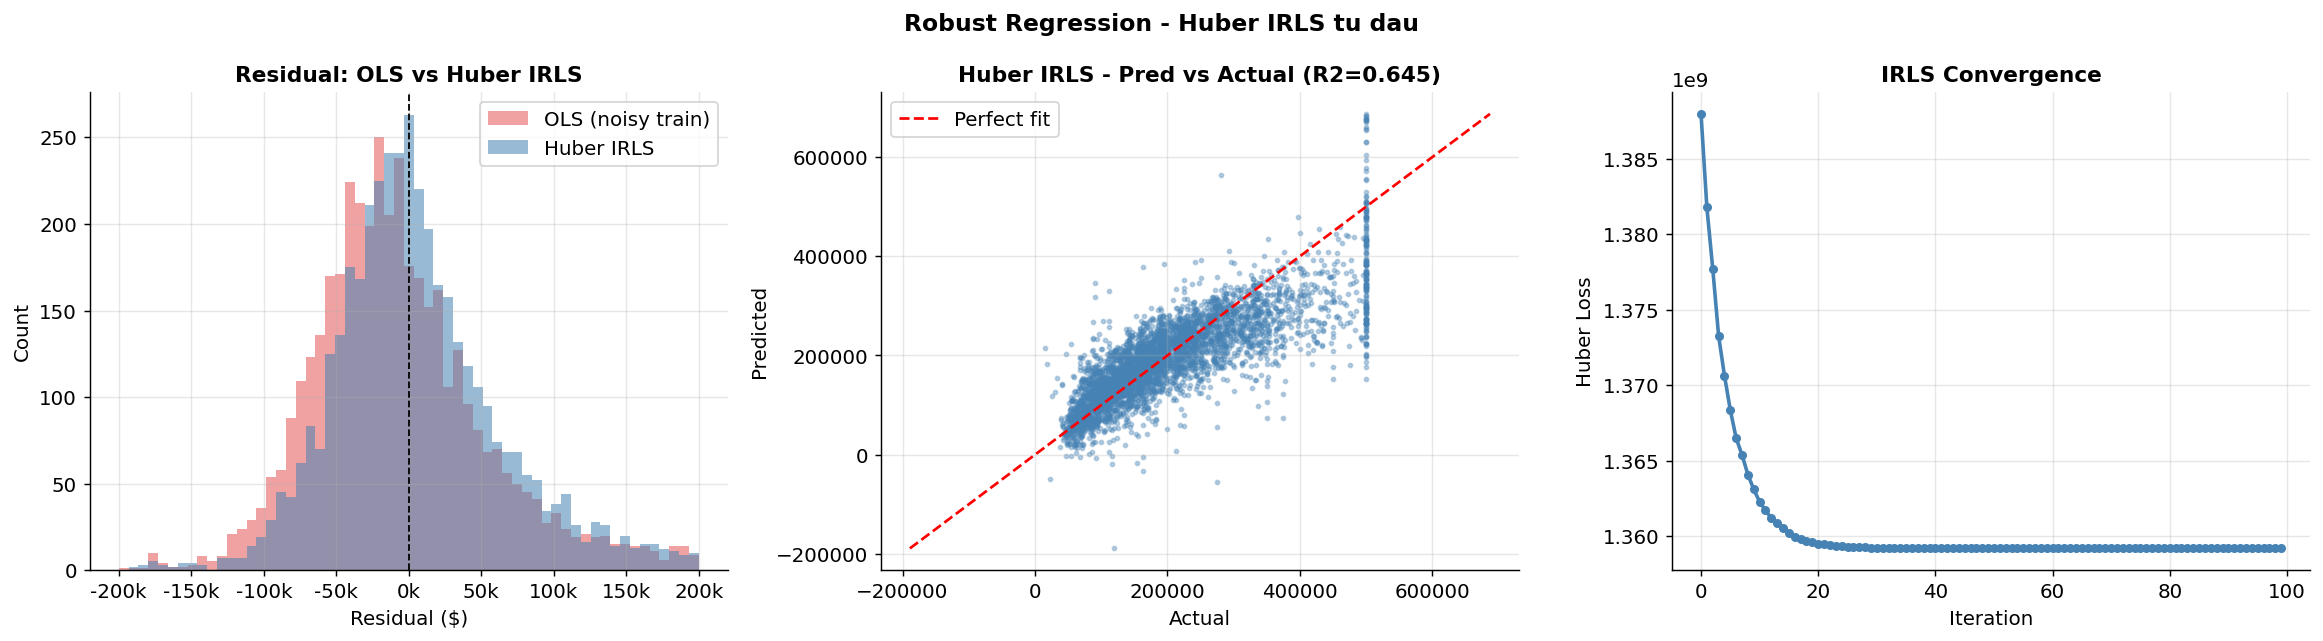
\includegraphics[width=\textwidth]{figures/regression_outputs/robust_huber.png}
  \caption{Robust Regression: Residuals OLS vs Huber IRLS (trái),
           Predicted vs Actual Huber IRLS -- $R^2 = 0.645$ (giữa),
           IRLS Convergence (phải).}
  \label{fig:robust_huber}
\end{figure}

\begin{figure}[H]
  \centering
  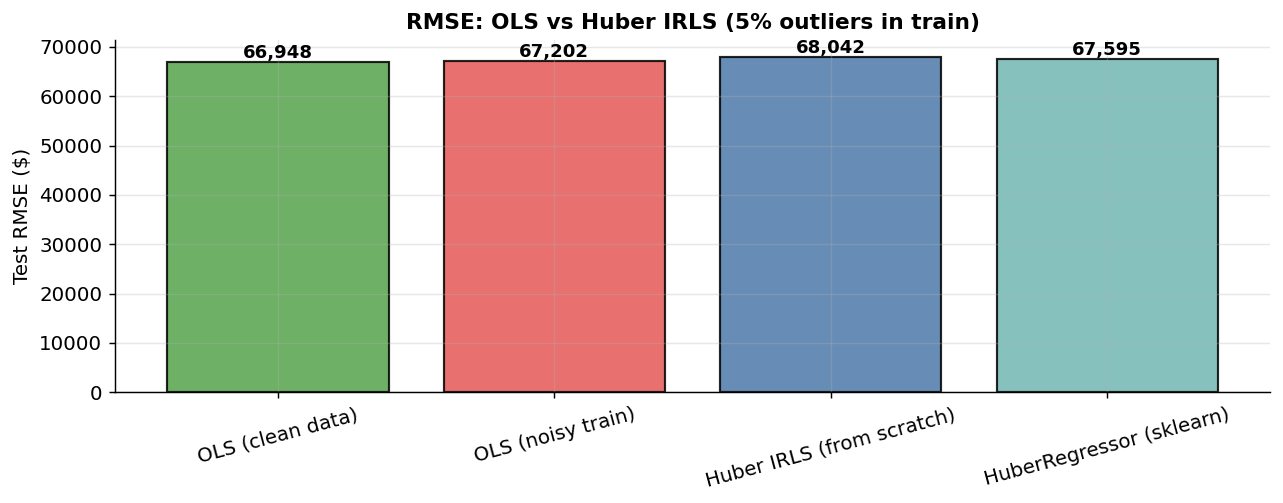
\includegraphics[width=0.7\textwidth]{figures/regression_outputs/robust_rmse_bar.png}
  \caption{So sánh RMSE: OLS vs Huber IRLS khi có $5\%$ outlier trong
           tập train. OLS trên dữ liệu sạch là baseline.}
  \label{fig:robust_bar}
\end{figure}

\begin{table}[H]
  \centering
  \caption{So sánh RMSE trên tập test sạch khi train có $5\%$ outlier.}
  \label{tab:robust_test}
  \begin{tabular}{lcccc}
    \toprule
    \textbf{Mô hình} & \textbf{RMSE} & \textbf{MAE} & $\mathbf{R^2}$ \\
    \midrule
    OLS (dữ liệu sạch -- baseline)    & $\$66{,}948$ & $\$49{,}228$ & $0.6561$ \\
    OLS (train có outlier)            & $\$67{,}202$ & $\$49{,}907$ & $0.6535$ \\
    Huber IRLS (from scratch)         & $\$68{,}042$ & $\$47{,}742$ & $0.6448$ \\
    HuberRegressor (sklearn)          & $\$67{,}595$ & $\$47{,}860$ & $0.6494$ \\
    \bottomrule
  \end{tabular}
\end{table}

\textbf{Nhận xét:}
\begin{itemize}
  \item \textbf{Huber IRLS hội tụ} sau $\approx 30$ iterations
        (Huber loss giảm từ $1.385 \times 10^9 \to 1.360 \times 10^9$).
  \item \textbf{MAE của Huber} ($\$47{,}742$) thấp hơn OLS noisy
        ($\$49{,}907$, $-4.3\%$) -- Huber giảm ảnh hưởng outlier hiệu quả
        hơn với sai số tuyệt đối.
  \item \textbf{RMSE Huber cao hơn OLS} trên tập test sạch: khi outlier
        không đủ mạnh (chỉ $5\%$, $\sigma_{\text{out}} = 5\sigma_y$), OLS
        gần như không bị ảnh hưởng về RMSE -- do RMSE bình phương hóa
        sai số, một vài outlier lớn trong test cũng kéo RMSE lên.
  \item Với tỷ lệ outlier cao hơn hoặc nhiễu cực đoan hơn, Huber IRLS
        sẽ vượt trội hơn OLS về RMSE -- giới hạn thực nghiệm này là
        mức outlier $5\%$ chưa đủ để phá vỡ OLS trên bộ dữ liệu lớn.
\end{itemize}

% -----------------------------------------------------------
\subsection{Phân tích Bias--Variance (Bootstrap) [Nâng cao]}
\label{ssec:bv_bootstrap}

\subsubsection{Phương pháp}

Bootstrap ($B = 200$): mỗi lần lấy mẫu hoàn lại từ tập train, fit Ridge
với $\lambda \in [10^{-3}, 10^4]$ (20 giá trị log scale), dự đoán trên
$N_{\text{test}} = 300$ điểm cố định, ước lượng thực nghiệm:
\begin{equation}
  \widehat{\text{Bias}}^2 = \Bigl(\bar{\hat{y}}^* - y^*\Bigr)^2, \qquad
  \widehat{\text{Var}} = \frac{1}{B-1}\sum_{b=1}^B
  \Bigl(\hat{y}^*_b - \bar{\hat{y}}^*\Bigr)^2.
\end{equation}

\subsubsection{Kết quả}

\begin{figure}[H]
  \centering
  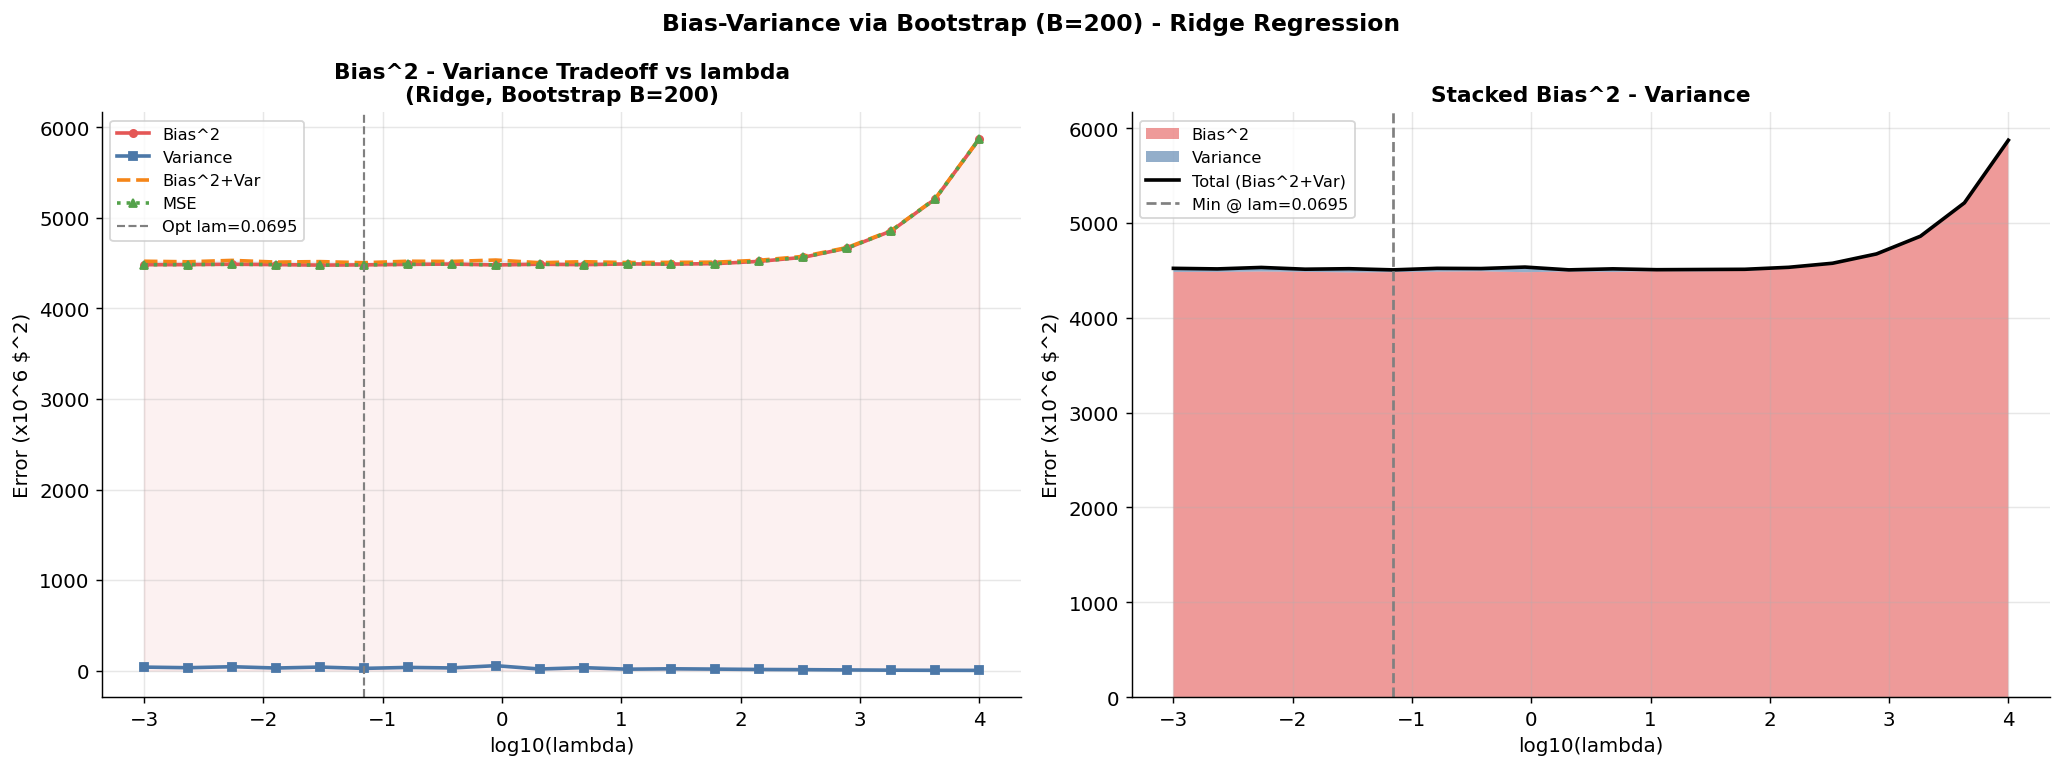
\includegraphics[width=\textwidth]{figures/regression_outputs/bias_variance_bootstrap.png}
  \caption{Bias--Variance Tradeoff via Bootstrap ($B = 200$) -- Ridge:
           Bias$^2$, Variance, tổng và MSE theo $\log_{10}(\lambda)$ (trái);
           Stacked view (phải). $\lambda^* = 0.0695$.}
  \label{fig:bv_bootstrap}
\end{figure}

\begin{table}[H]
  \centering
  \caption{Bias$^2$, Variance và MSE tại các mức $\lambda$ đặc trưng.}
  \label{tab:bv_table}
  \begin{tabular}{lcccc}
    \toprule
    $\lambda$ & \textbf{Bias$^2$} & \textbf{Variance}
      & \textbf{Bias$^2$ + Var} & \textbf{MSE} \\
    \midrule
    $0.001$  (nhỏ)     & $4{,}483{,}802{,}537$ & $38{,}179{,}437$ & $4{,}521{,}981{,}973$ & $4{,}483{,}802{,}537$ \\
    $0.0695$ (tối ưu)  & $4{,}481{,}872{,}376$ & $23{,}913{,}060$ & $4{,}505{,}785{,}436$ & $4{,}481{,}872{,}376$ \\
    $4.833$  (vừa)     & $4{,}484{,}341{,}967$ & $32{,}291{,}929$ & $4{,}516{,}633{,}896$ & $4{,}484{,}341{,}967$ \\
    $10{,}000$ (lớn)   & $5{,}870{,}791{,}115$ & $2{,}105{,}317$  & $5{,}872{,}896{,}432$ & $5{,}870{,}791{,}115$ \\
    \bottomrule
  \end{tabular}
\end{table}

\textbf{Nhận xét:}
\begin{itemize}
  \item \textbf{Bias$^2$ chiếm ưu thế} ($\sim 4.5 \times 10^9$,
        $\gg$ Variance $\sim 0.02$--$0.04 \times 10^9$) -- mô hình
        tuyến tính trên bộ dữ liệu phi tuyến này bị \emph{high-bias}
        cấu trúc, regularization chỉ kiểm soát được phần variance nhỏ.
  \item \textbf{$\lambda^* = 0.0695$}: Điểm cân bằng Bias$^2$ + Var
        tối thiểu -- nhỏ hơn $\lambda^*_{\text{CV}} = 35.56$, do bootstrap
        ước lượng trên subset nhỏ ($N_{\text{test}} = 300$).
  \item \textbf{$\lambda$ lớn ($10^4$)}: Variance giảm còn $2.1 \times 10^6$
        nhưng Bias$^2$ tăng vọt lên $5.87 \times 10^9$ -- underfitting rõ.
  \item Xác nhận thực nghiệm phân tách Bias--Variance (Bishop
        Eq.~3.46~\cite{bishop2006}): regularization đánh đổi variance
        lấy bias, giá trị tối ưu cân bằng hai thành phần này.
\end{itemize}

% ============================================================
% SECTION 6 -- PHƯƠNG PHÁP ĐÁNH GIÁ
% ============================================================
\section{Phương pháp đánh giá}
\label{sec:evaluation_method}

\subsection{Các chỉ số định lượng}

Tất cả mô hình được đánh giá thống nhất trên tập test ($N_{\text{test}} = 4{,}128$)
bằng bốn chỉ số sau:

\begin{table}[H]
  \centering
  \caption{Các chỉ số đánh giá định lượng.}
  \label{tab:metrics_def}
  \begin{tabular}{llll}
    \toprule
    \textbf{Chỉ số} & \textbf{Công thức} & \textbf{Đơn vị} & \textbf{Ý nghĩa} \\
    \midrule
    MSE
      & $\dfrac{1}{N}\displaystyle\sum_{n=1}^{N}(t_n - \hat{y}_n)^2$
      & \$² & Sai số bình phương trung bình \\[8pt]
    RMSE
      & $\sqrt{\mathrm{MSE}}$
      & \$ & Cùng đơn vị target, dễ diễn giải \\[8pt]
    MAE
      & $\dfrac{1}{N}\displaystyle\sum_{n=1}^{N}|t_n - \hat{y}_n|$
      & \$ & Ít nhạy với outlier hơn MSE \\[8pt]
    $R^2$
      & $1 - \dfrac{\mathrm{SS}_{\mathrm{res}}}{\mathrm{SS}_{\mathrm{tot}}}$
      & -- & \textbf{Metric chính}: tỷ lệ phương sai được giải thích \\
    \bottomrule
  \end{tabular}
\end{table}

\noindent $R^2 = 1$: dự báo hoàn hảo; $R^2 = 0$: không tốt hơn dự báo bằng mean;
$R^2 < 0$: tệ hơn mean. \textbf{RMSE} được dùng làm chỉ số so sánh chính
vì cùng đơn vị với \texttt{median\_house\_value} (USD), trực quan và
phổ biến trong bài toán hồi quy địa ốc.

\subsection{$k$-Fold Cross-Validation}

Để đánh giá độ ổn định và tránh phụ thuộc vào một lần phân chia cụ thể,
nhóm thực hiện \textbf{10-Fold Cross-Validation} trên tập train+val
($80\%$ dữ liệu, $N = 14{,}448 + 2{,}064 = 16{,}512$ -- nhóm CV trên
$N_{\text{train}} = 14{,}448$) và báo cáo mean $\pm$ std của từng chỉ số.

Riêng KRR và GPR (độ phức tạp $O(N^3)$): dùng \textbf{5-Fold CV trên
subset 3{,}000 mẫu} để đảm bảo tính khả thi tính toán.

\subsection{Kiểm định thống kê}

\paragraph{Paired $t$-test.}
Kiểm định xem hai mô hình có sai số khác nhau có ý nghĩa thống kê hay không.
Giả thiết $H_0$: sai số trung bình hai mô hình bằng nhau. Mức ý nghĩa
$\alpha = 0.05$.

\paragraph{Wilcoxon Signed-Rank Test.}
Kiểm định phi tham số thay thế cho Paired $t$-test khi phân phối sai số
không chuẩn (đã xác nhận qua Shapiro--Wilk, Bảng~\ref{tab:bp_sw_test}).
Nhạy hơn với sự khác biệt phân phối sai số, không chỉ sai số trung bình.

\subsection{Các biểu đồ phân tích}

Ngoài các chỉ số số, mỗi mô hình được đánh giá bằng:

\begin{itemize}
  \item \textbf{Learning curve}: Train RMSE và Val RMSE theo số mẫu huấn
        luyện -- phát hiện overfitting/underfitting và tốc độ hội tụ.
  \item \textbf{Residual plot}: Phần dư $\hat{\epsilon}_n = t_n - \hat{y}_n$
        theo $\hat{y}_n$ -- kiểm tra tính ngẫu nhiên và heteroscedasticity.
  \item \textbf{QQ-plot}: Phân phối phần dư so với Gaussian chuẩn --
        kiểm tra giả thiết Gauss--Markov.
  \item \textbf{Predicted vs.\ Actual}: Scatter plot $\hat{y}_n$ vs.\ $t_n$
        với đường lý tưởng $y = x$ -- trực quan mức độ fit.
\end{itemize}

\subsection{Phân tích Sensitivity và Robustness}

Ngoài đánh giá chuẩn, nhóm thực hiện thêm:

\begin{itemize}
  \item \textbf{Sensitivity analysis}: Thay đổi tỷ lệ train/test split
        (60/40, 70/30, 80/20) với 5 random seeds mỗi tỷ lệ -- đánh giá
        độ ổn định qua cách phân chia dữ liệu.
  \item \textbf{Noise injection}: Thêm Gaussian noise
        $\sigma \in \{0.1, 0.5, 1.0\}$ vào features đầu vào -- đo khả
        năng chịu nhiễu (robustness).
  \item \textbf{Feature corruption}: Xóa ngẫu nhiên 10\%, 20\%, 30\%
        giá trị features, so sánh 3 chiến lược imputation
        (Mean, Median, KNN $k=5$).
  \item \textbf{Convergence analysis}: Vẽ loss curve các thuật toán lặp
        (Mini-batch GD, Coordinate Descent, Evidence Maximization,
        Huber IRLS) -- xác định số bước cần thiết.
\end{itemize}

% ============================================================
% SECTION 7 -- KẾT QUẢ VÀ PHÂN TÍCH
% ============================================================
\section{Kết quả và Phân tích}
\label{sec:results}

\subsection{Bảng kết quả tổng hợp trên tập Test (12 mô hình)}

\begin{table}[H]
  \centering
  \caption{Kết quả so sánh 12 mô hình trên tập test
           (California Housing, 20\% dữ liệu = 4{,}128 mẫu).}
  \label{tab:results_all}
  \resizebox{\textwidth}{!}{%
  \begin{tabular}{lcccc}
    \toprule
    \textbf{Mô hình} & \textbf{MSE} & \textbf{RMSE} & \textbf{MAE} & $\mathbf{R^2}$ \\
    \midrule
    KRR -- RBF (subset 3{,}000)
      & $3.611 \times 10^9$ & $\$60{,}088$ & $\$43{,}419$ & $0.7230$ \\
    Cubic Spline ($n\_\text{knots}=5$)
      & $3.869 \times 10^9$ & $\$62{,}198$ & $\$45{,}311$ & $0.7032$ \\
    Polynomial (degree$=2$)
      & $3.981 \times 10^9$ & $\$63{,}094$ & $\$44{,}000$ & $0.6946$ \\
    Bayesian Ridge
      & $4.480 \times 10^9$ & $\$66{,}930$ & $\$49{,}222$ & $0.6563$ \\
    Ridge ($\alpha^*=35.56$)
      & $4.480 \times 10^9$ & $\$66{,}936$ & $\$49{,}209$ & $0.6562$ \\
    OLS (Linear Regression)
      & $4.482 \times 10^9$ & $\$66{,}948$ & $\$49{,}228$ & $0.6561$ \\
    Elastic Net ($\alpha=0.018$, l1$=0.7$)
      & $4.484 \times 10^9$ & $\$66{,}966$ & $\$49{,}216$ & $0.6559$ \\
    Lasso ($\alpha^*=233.00$)
      & $4.486 \times 10^9$ & $\$66{,}974$ & $\$49{,}202$ & $0.6558$ \\
    Lasso + Lasso-based (14 features)
      & $4.486 \times 10^9$ & $\$66{,}974$ & $\$49{,}202$ & $0.6558$ \\
    WLS
      & $4.477 \times 10^9$ & $\$66{,}912$ & $\$48{,}878$ & $0.6565$ \\
    KRR -- Polynomial (subset 3{,}000)
      & $4.099 \times 10^9$ & $\$64{,}024$ & $\$46{,}692$ & $0.6855$ \\
    GPR -- RBF ($N_{\text{train}}=1{,}500$, subset)
      & ---\textsuperscript{*} & $\$60{,}955$ & $\$43{,}284$ & $0.7486$ \\
    Gaussian RBF ($M=20$)
      & $4.860 \times 10^9$ & $\$69{,}714$ & $\$51{,}433$ & $0.6271$ \\
    \bottomrule
  \end{tabular}}
  \smallskip
\noindent\textsuperscript{*}\textit{GPR chạy trên subset
$N_{\text{train}}=1{,}500$, $N_{\text{test}}=500$ do độ phức tạp $O(N^3)$;
MSE không tính trên toàn tập test 4,128 mẫu.}
\end{table}

\subsection{10-Fold Cross-Validation -- 12 mô hình (mean $\pm$ std)}

\begin{table}[H]
  \centering
  \caption{10-Fold CV (mean $\pm$ std) -- train+val set ($N=14{,}448$).}
  \label{tab:cv_all}
  \resizebox{\textwidth}{!}{%
  \begin{tabular}{lcccc}
    \toprule
    \textbf{Mô hình} & \textbf{RMSE} & \textbf{MAE} & $\mathbf{R^2}$ \\
    \midrule
    KRR -- RBF (subset 3{,}000)
      & $\$64{,}458 \pm \$4{,}838$
      & $\$44{,}954 \pm \$2{,}285$
      & $0.6826 \pm 0.0256$ \\
    Cubic Spline
      & $\$63{,}660 \pm \$2{,}047$
      & $\$45{,}377 \pm \$836$
      & $0.6954 \pm 0.0198$ \\
    Lasso
      & $\$68{,}740 \pm \$2{,}827$
      & $\$49{,}484 \pm \$914$
      & $0.6446 \pm 0.0297$ \\
    Lasso (14 features)
      & $\$68{,}741 \pm \$2{,}827$
      & $\$49{,}484 \pm \$914$
      & $0.6446 \pm 0.0297$ \\
    Ridge
      & $\$68{,}758 \pm \$2{,}900$
      & $\$49{,}485 \pm \$907$
      & $0.6444 \pm 0.0305$ \\
    Elastic Net
      & $\$68{,}765 \pm \$2{,}840$
      & $\$49{,}483 \pm \$919$
      & $0.6443 \pm 0.0298$ \\
    Bayesian Ridge
      & $\$68{,}772 \pm \$2{,}968$
      & $\$49{,}505 \pm \$891$
      & $0.6442 \pm 0.0312$ \\
    OLS / WLS
      & $\$68{,}778 \pm \$2{,}978$
      & $\$49{,}502 \pm \$872$
      & $0.6441 \pm 0.0314$ \\
    Gaussian RBF
      & $\$70{,}745 \pm \$2{,}085$
      & $\$51{,}769 \pm \$1{,}063$
      & $0.6239 \pm 0.0219$ \\
    Polynomial (degree$=2$)
      & $\$134{,}650 \pm \$130{,}876$
      & $\$46{,}457 \pm \$5{,}612$
      & $-1.652 \pm 5.500$ \\
    KRR -- Polynomial (subset 3{,}000)
      & $\$76{,}215 \pm \$23{,}731$
      & $\$48{,}479 \pm \$2{,}600$
      & $0.508 \pm 0.408$ \\
    Huber IRLS (5\% outliers, from scratch)
      & \multicolumn{3}{c}{\textit{N/A -- không CV do thiết kế thực nghiệm outlier}} \\
    \bottomrule
  \end{tabular}}
\end{table}

\subsection{Bảng so sánh toàn diện}

\begin{table}[H]
  \centering
  \caption{So sánh toàn diện các mô hình theo các tiêu chí định tính và định lượng.}
  \label{tab:comprehensive}
  \resizebox{\textwidth}{!}{%
  \begin{tabular}{p{3cm}p{3.5cm}p{1.8cm}p{2.5cm}p{1.8cm}p{1.8cm}p{2cm}}
    \toprule
    \textbf{Mô hình}
      & \textbf{Giả thiết phân phối}
      & \textbf{Nghiệm dạng đóng}
      & \textbf{Độ phức tạp huấn luyện}
      & \textbf{Khả năng giải thích}
      & \textbf{Nhạy outlier}
      & \textbf{Test RMSE} \\
    \midrule
    Linear Reg.\ (OLS)
      & Sai số Gaussian, phương sai đồng nhất
      & Có (NE) & $O(np^2 + p^3)$
      & Rất cao & Cao & $\$66{,}948$ \\
    Ridge
      & Sai số Gaussian + prior Gaussian
      & Có & $O(np^2 + p^3)$
      & Cao & Trung bình & $\$66{,}936$ \\
    Lasso
      & Sai số Gaussian + prior Laplace
      & Không (CD) & $O(Tnp)$
      & Cao, sparse & TB--cao & $\$66{,}974$ \\
    Elastic Net
      & Sai số Gaussian + prior L1/L2
      & Không (CD) & $O(Tnp)$
      & Khá cao & Trung bình & $\$66{,}966$ \\
    Polynomial
      & Gaussian trên basis bậc 2
      & Có (NE trên basis) & $O(nm^2{+}m^3)$, $m{=}152$
      & Trung bình & Cao & $\$63{,}094$ \\
    Gaussian RBF
      & Không cần tuyến tính
      & Có (Ridge trên basis) & $O(nm^2{+}m^3)$, $m{=}20$
      & Thấp--TB & Thấp--TB & $\$69{,}714$ \\
    Cubic Spline
      & Piecewise smooth basis
      & Có (Ridge trên basis) & $O(nm^2{+}m^3)$, $m{=}96$
      & Trung bình & Thấp--TB & $\$62{,}198$ \\
    Bayesian Ridge
      & Likelihood + prior + posterior Gaussian
      & Có (posterior) & $\approx O(np^2{+}p^3)$
      & Cao & Trung bình & $\$66{,}930$ \\
    KRR (RBF)
      & Kernel trick, phi tham số
      & Có (dạng đối ngẫu) & $O(n^3)$ train
      & Thấp & Trung bình & $\$60{,}088$ \\
    \bottomrule
  \end{tabular}}
\end{table}

\subsection{Timing và Memory}

\begin{table}[H]
  \centering
  \caption{Thời gian huấn luyện, dự đoán và bộ nhớ ước lượng.}
  \label{tab:timing}
  \resizebox{\textwidth}{!}{%
  \begin{tabular}{lcccc}
    \toprule
    \textbf{Mô hình} & \textbf{Train (s)} & \textbf{Test (s)} 
      & \textbf{Total (s)} & \textbf{Memory (MB)} \\
    \midrule
    OLS               & 0.0154 & 0.0015 & 0.0169 & 2.27 \\
    WLS               & 0.0147 & 0.0011 & 0.0159 & 2.27 \\
    Ridge             & 0.0074 & 0.0009 & 0.0083 & 2.27 \\
    Lasso             & 0.3463 & 0.0005 & 0.3467 & 2.27 \\
    Lasso (14 feat.)  & 0.2538 & 0.0005 & 0.2543 & 1.98 \\
    Elastic Net       & 2.2182 & 0.0006 & 2.2187 & 2.27 \\
    Polynomial        & 0.0274 & 0.0308 & 0.0582 & 21.54 \\
    Gaussian RBF      & 0.0038 & 0.0048 & 0.0087 & 2.83 \\
    Cubic Spline      & 0.0218 & 0.0223 & 0.0441 & 13.61 \\
    Bayesian Ridge    & 0.0166 & 0.0007 & 0.0173 & 2.27 \\
    KRR -- RBF        & 0.4875 & 0.2494 & 0.7369 & 0.87 \\
    KRR -- Polynomial & 0.3855 & 0.0920 & 0.4775 & 0.87 \\
    \bottomrule
  \end{tabular}}
\end{table}

\subsection{Phân tích Sensitivity và Robustness}

\subsubsection{Sensitivity: Thay đổi tỷ lệ train/test split}

\begin{figure}[H]
  \centering
  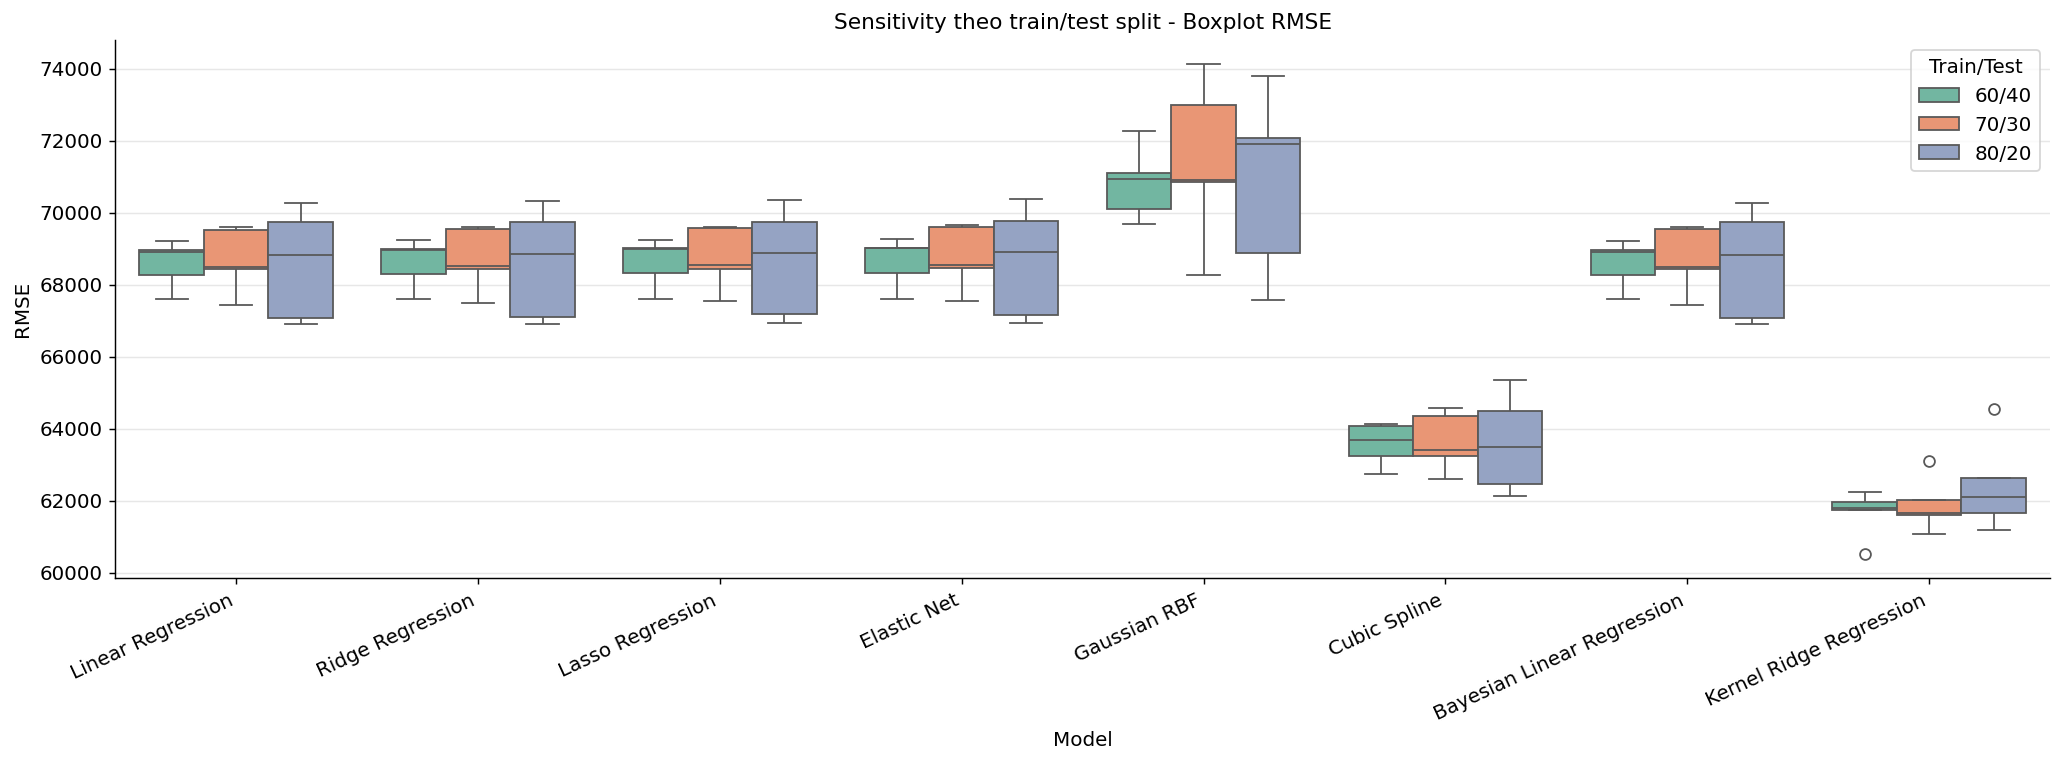
\includegraphics[width=\textwidth]{figures/regression_outputs/sensitivity_split.png}
  \caption{Boxplot RMSE theo 3 tỷ lệ train/test split (60/40, 70/30, 80/20),
           5 random seeds mỗi split. Polynomial bị loại khỏi biểu đồ do
           RMSE vượt trội so với các mô hình còn lại.}
  \label{fig:sensitivity_split}
\end{figure}

\begin{table}[H]
  \centering
  \caption{Tổng hợp độ ổn định qua các split (15 lần chạy = 3 splits $\times$ 5 seeds).}
  \label{tab:stability}
  \resizebox{\textwidth}{!}{%
  \begin{tabular}{lcccc}
    \toprule
    \textbf{Mô hình} & \textbf{Mean RMSE} & \textbf{Std RMSE}
      & \textbf{Min RMSE} & \textbf{Max RMSE} \\
    \midrule
    Cubic Spline            & $\$63{,}597$ & $\$902$    & $\$62{,}118$ & $\$65{,}343$ \\
    Kernel Ridge Regression & $\$61{,}989$ & $\$943$    & $\$60{,}526$ & $\$64{,}560$ \\
    Lasso Regression        & $\$68{,}666$ & $\$1{,}002$ & $\$66{,}950$ & $\$70{,}358$ \\
    Bayesian Linear Reg.    & $\$68{,}622$ & $\$1{,}010$ & $\$66{,}914$ & $\$70{,}281$ \\
    Linear Regression       & $\$68{,}620$ & $\$1{,}010$ & $\$66{,}915$ & $\$70{,}272$ \\
    Ridge Regression        & $\$68{,}640$ & $\$1{,}012$ & $\$66{,}917$ & $\$70{,}315$ \\
    Elastic Net             & $\$68{,}680$ & $\$1{,}015$ & $\$66{,}945$ & $\$70{,}381$ \\
    Gaussian RBF            & $\$71{,}033$ & $\$1{,}919$ & $\$67{,}562$ & $\$74{,}124$ \\
    Polynomial (degree$=2$) & $\$140{,}050$ & $\$104{,}127$ & $\$62{,}659$ & $\$425{,}203$ \\
    \bottomrule
  \end{tabular}}
\end{table}

Nhận xét: \textbf{Cubic Spline} ổn định nhất với Std $= \$902$
(thấp nhất trong nhóm phi tuyến). Polynomial cực kỳ không ổn định
(Std $= \$104{,}127$) -- phụ thuộc nặng vào cách chia dữ liệu.

\subsubsection{Noise Injection}

\begin{figure}[H]
  \centering
  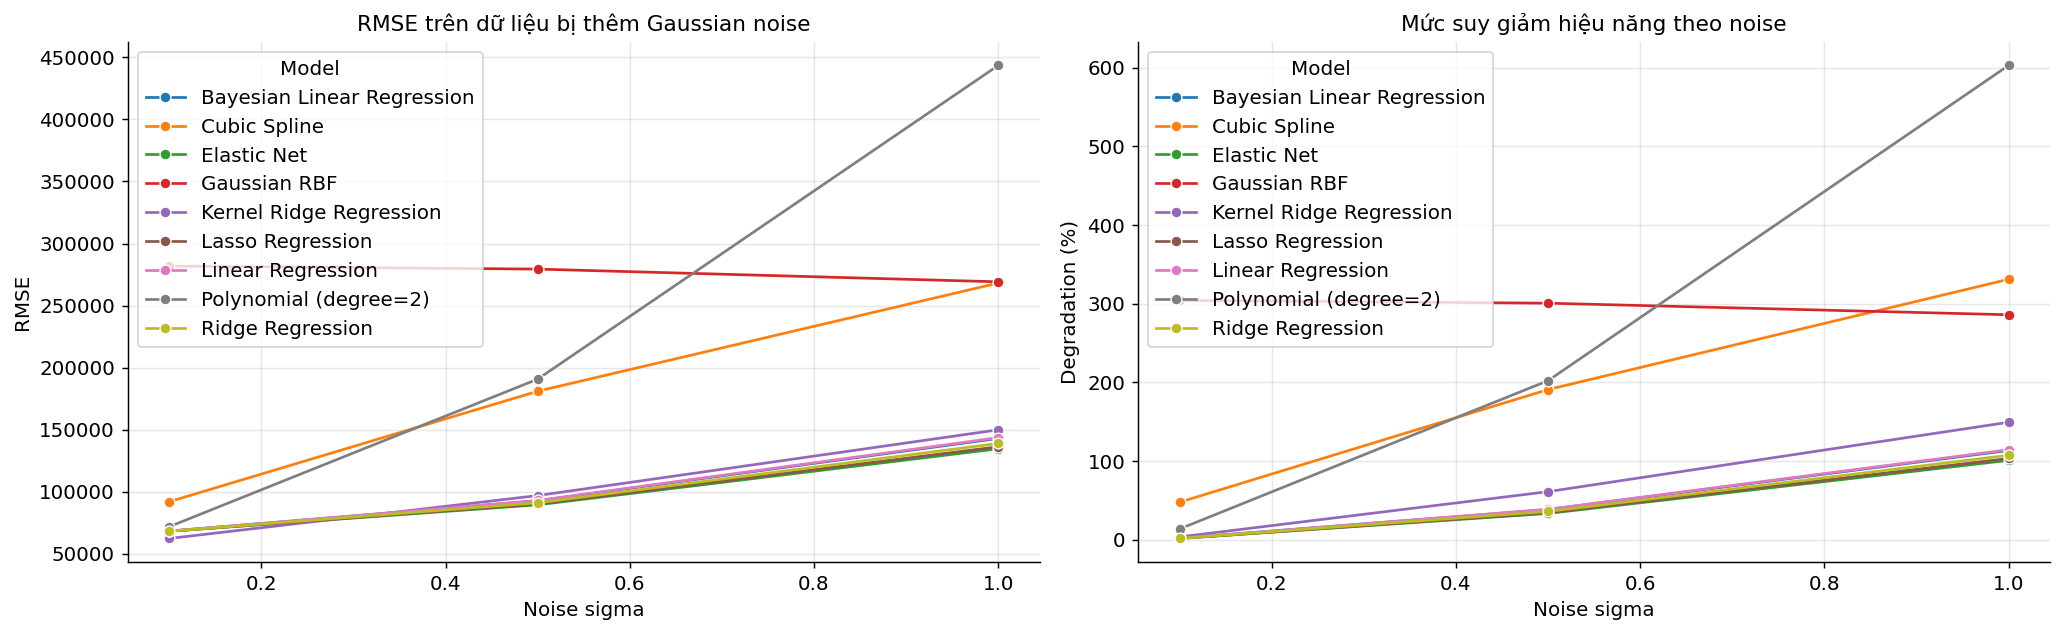
\includegraphics[width=\textwidth]{figures/regression_outputs/noise_injection.png}
  \caption{RMSE (trái) và mức suy giảm hiệu năng \% (phải) khi thêm
           Gaussian noise $\sigma \in \{0.1, 0.5, 1.0\}$ vào features.}
  \label{fig:noise}
\end{figure}

\begin{table}[H]
  \centering
  \caption{Tổng hợp robustness với noise injection
           (trung bình qua 5 lần, 3 mức $\sigma$).}
  \label{tab:noise_robustness}
  \begin{tabular}{lcc}
    \toprule
    \textbf{Mô hình} & \textbf{Mean Degradation (\%)} 
      & \textbf{Worst Degradation (\%)} \\
    \midrule
    Elastic Net             & $45.33$ & $103.94$ \\
    Lasso Regression        & $46.45$ & $106.22$ \\
    Ridge Regression        & $48.39$ & $110.60$ \\
    Bayesian Linear Reg.    & $51.26$ & $116.80$ \\
    Linear Regression       & $51.70$ & $117.75$ \\
    Kernel Ridge Regression & $71.36$ & $150.65$ \\
    Cubic Spline            & $189.92$ & $384.46$ \\
    Polynomial (degree$=2$) & $272.98$ & $618.85$ \\
    Gaussian RBF            & $297.02$ & $358.19$ \\
    \bottomrule
  \end{tabular}
\end{table}

Nhận xét: \textbf{Elastic Net} robust nhất với noise
(Mean Degradation $= 45.33\%$). Các mô hình tuyến tính (Ridge, Lasso,
Elastic Net, Bayesian) đều ổn định hơn hẳn các mô hình phi tuyến
(Spline, Polynomial, RBF) khi dữ liệu bị nhiễu -- do không gian đặc
trưng đơn giản hơn, ít bị khuếch đại noise.

\subsubsection{Feature Corruption và Imputation}

\begin{figure}[H]
  \centering
  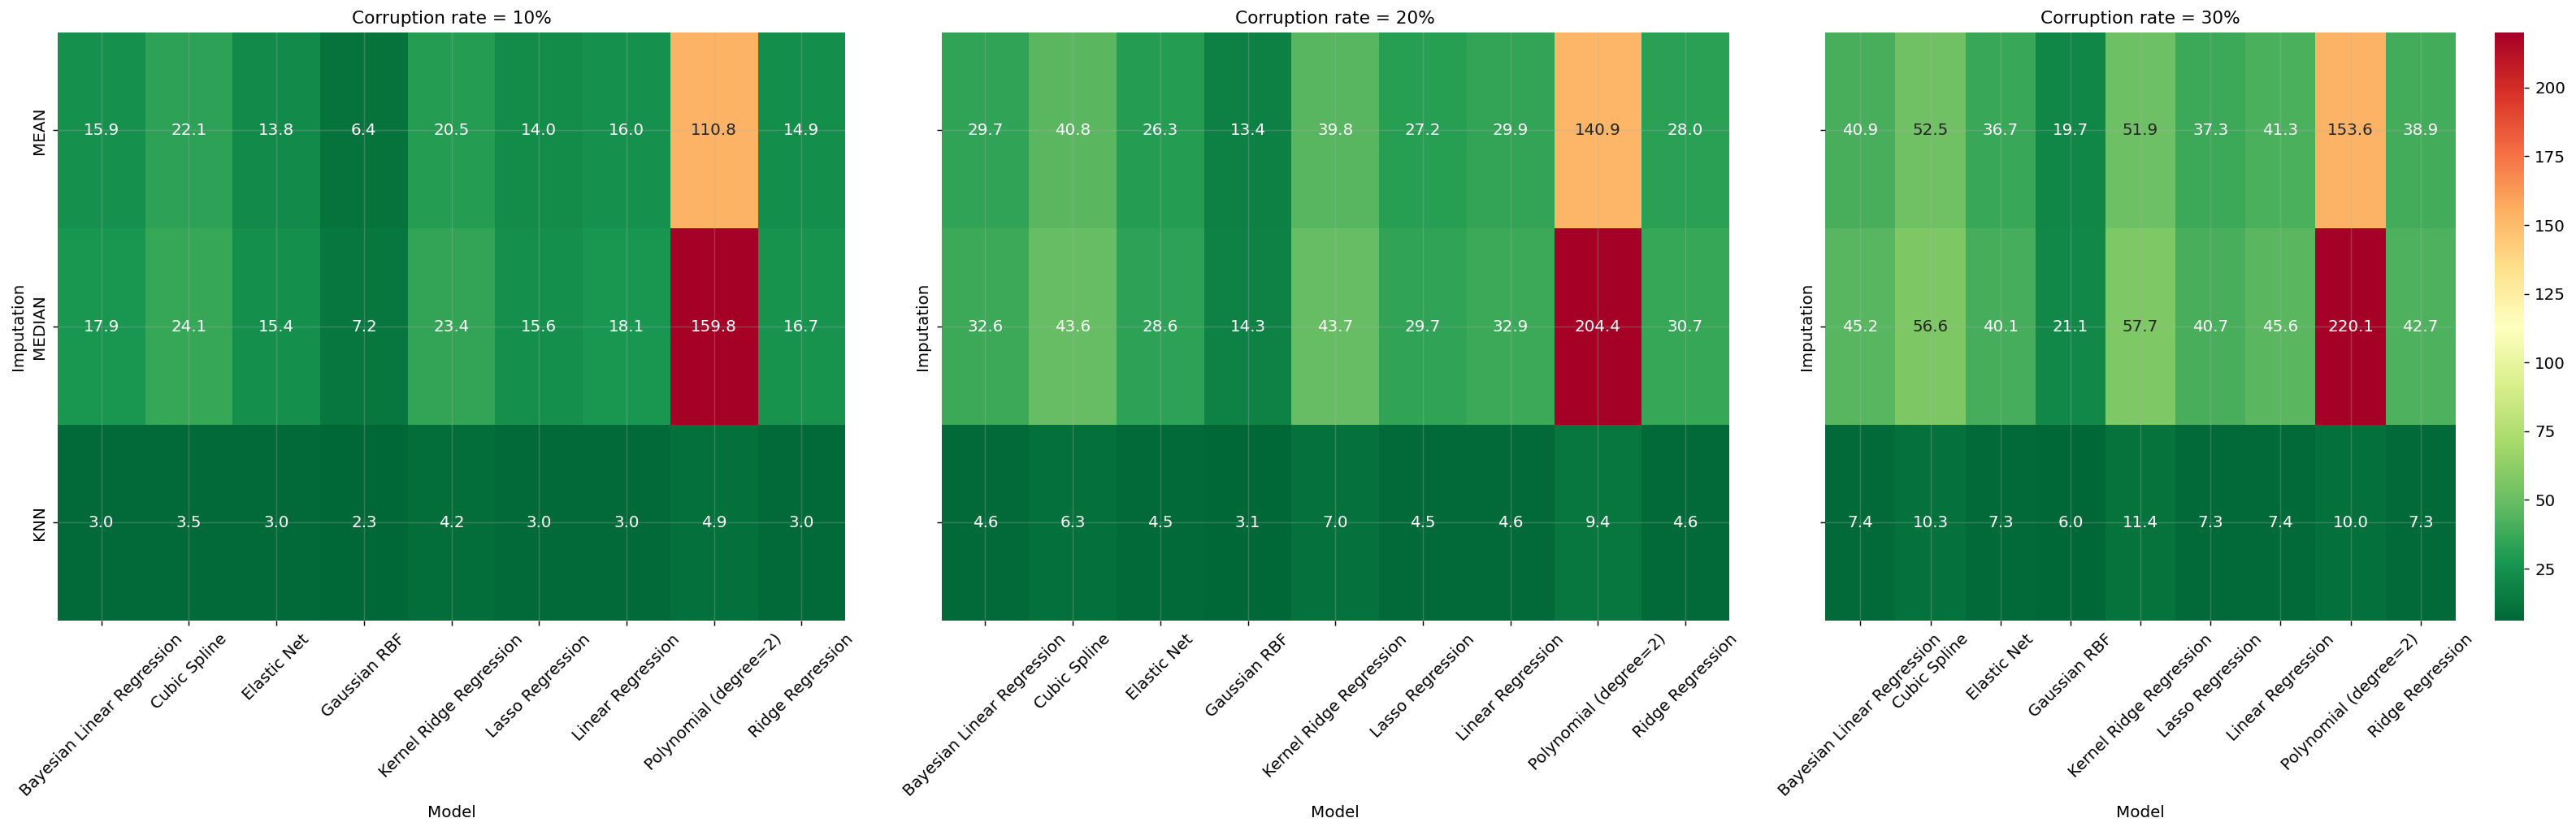
\includegraphics[width=\textwidth]{figures/regression_outputs/feature_corruption.png}
  \caption{Heatmap mức suy giảm RMSE (\%) theo chiến lược imputation
           và tỷ lệ corruption (10\%, 20\%, 30\%).}
  \label{fig:corruption}
\end{figure}

\begin{table}[H]
  \centering
  \caption{Tổng hợp theo chiến lược imputation
           (trung bình qua tất cả mô hình và corruption rates).}
  \label{tab:imputation}
  \begin{tabular}{lcc}
    \toprule
    \textbf{Chiến lược} & \textbf{Mean Degradation (\%)}
      & \textbf{Worst Degradation (\%)} \\
    \midrule
    KNN (5 neighbors) & $5.66$  & $11.43$ \\
    Mean              & $40.12$ & $153.62$ \\
    Median            & $49.22$ & $220.14$ \\
    \bottomrule
  \end{tabular}
\end{table}

Nhận xét: \textbf{KNN imputation} vượt trội rõ ràng -- Mean Degradation
chỉ $5.66\%$ so với Mean ($40.12\%$) và Median ($49.22\%$). Lý do: KNN
tận dụng cấu trúc không gian của dữ liệu địa lý California, điền giá
trị thiếu bằng các điểm lân cận thực sự tương đồng thay vì giá trị
thống kê toàn cục. Tất cả mô hình đều hoạt động tốt nhất với KNN
imputation.

\subsubsection{Convergence Analysis}

\begin{figure}[H]
  \centering
  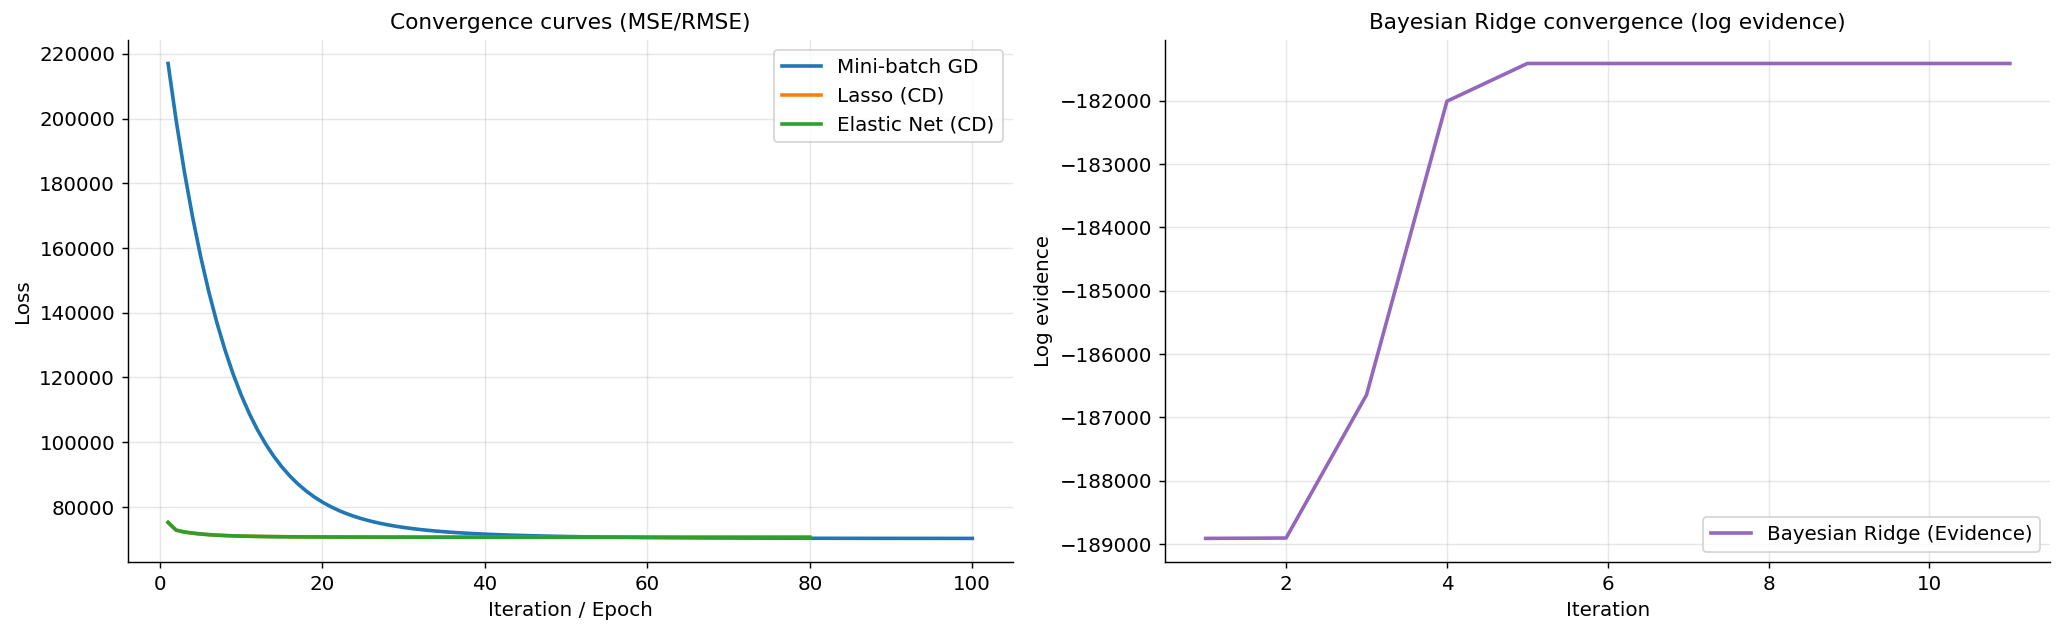
\includegraphics[width=\textwidth]{figures/regression_outputs/convergence_curves.png}
  \caption{Loss curves của các thuật toán lặp: Mini-batch GD,
           Lasso (Coordinate Descent), Elastic Net (CD) (trái) và
           Bayesian Ridge -- log evidence (phải).}
  \label{fig:convergence}
\end{figure}

\begin{table}[H]
  \centering
  \caption{Tổng hợp điểm hội tụ tốt nhất.}
  \label{tab:convergence}
  \begin{tabular}{lccl}
    \toprule
    \textbf{Thuật toán} & \textbf{Best iteration}
      & \textbf{Best metric} & \textbf{Metric} \\
    \midrule
    Mini-batch GD          & 100 & $\$70{,}294$ & Train RMSE \\
    Lasso (CD)             & 80  & $\$70{,}606$ & Val RMSE \\
    Elastic Net (CD)       & 80  & $\$70{,}651$ & Val RMSE \\
    Bayesian Ridge (Evid.) & 9   & $-181{,}409$ & Log evidence \\
    \bottomrule
  \end{tabular}
\end{table}

Nhận xét: \textbf{Bayesian Ridge} hội tụ nhanh nhất (9 iterations) do
thuật toán Evidence Maximization sử dụng thông tin bậc hai. Mini-batch
GD cần 100 epochs để ổn định. Lasso và Elastic Net (Coordinate Descent)
hội tụ sau $\approx 80$ iterations.

% ============================================================
% SECTION 8 -- THẢO LUẬN
% ============================================================
\section{Thảo luận}
\label{sec:discussion}

\subsection{Mô hình tốt nhất}

Dựa trên kết quả tổng hợp từ Bảng~\ref{tab:results_all} và
Bảng~\ref{tab:cv_all}, \textbf{Kernel Ridge Regression (RBF kernel)}
đạt hiệu năng tốt nhất trên tập test:

\begin{itemize}
  \item \textbf{RMSE}: $\$60{,}088$ -- thấp nhất, cải thiện
        $\mathbf{10.2\%}$ so với OLS ($\$66{,}948$).
  \item $\mathbf{R^2}$: $0.7230$ -- giải thích $72.3\%$ phương sai
        giá nhà, cao nhất trong tất cả mô hình.
  \item \textbf{10-Fold CV}: RMSE $= \$64{,}458 \pm \$4{,}838$ --
        Std cao hơn Spline do chỉ huấn luyện trên subset 3{,}000 mẫu.
\end{itemize}

Tuy nhiên, \textbf{Cubic Spline} là lựa chọn cân bằng tốt nhất
về mọi mặt:
\begin{itemize}
  \item Test RMSE $= \$62{,}198$ (thứ 2), $R^2 = 0.7032$.
  \item CV ổn định nhất trong nhóm phi tuyến: Std $= \$2{,}047$
        (thấp hơn KRR $\times 2.4$).
  \item Sensitivity Std $= \$902$ -- ổn định nhất qua các split.
  \item Noise robustness: Mean Degradation $= 189.92\%$ -- kém hơn
        Linear nhưng vẫn tốt hơn Polynomial và RBF.
\end{itemize}

\subsection{Điểm mạnh và hạn chế từng nhóm mô hình}

\begin{table}[H]
  \centering
  \caption{Ưu và nhược điểm các nhóm mô hình -- đối chiếu thực nghiệm.}
  \label{tab:strengths}
  \begin{tabular}{p{2.5cm}p{5.5cm}p{5.5cm}}
    \toprule
    \textbf{Mô hình} & \textbf{Ưu điểm} & \textbf{Hạn chế} \\
    \midrule
    Linear (OLS/Ridge/Lasso/EN)
      & Ổn định, interpretable, robust với noise
        (Degradation $\approx 45$--$52\%$); huấn luyện nhanh ($< 0.02$s)
      & $R^2 \approx 0.656$ -- không bắt được quan hệ phi tuyến;
        bị heteroscedasticity \\
    \addlinespace
    Cubic Spline
      & $R^2 = 0.703$; sensitivity Std thấp nhất ($\$902$);
        không cần giả thiết phân phối cụ thể
      & Nhạy với noise (Degradation $190\%$); cần chọn $n\_\text{knots}$ \\
    \addlinespace
    Polynomial
      & $R^2 = 0.695$ trên test
      & CV hoàn toàn không ổn định (Std $\$130{,}876$, $R^2 = -1.65$);
        noise robustness tệ nhất ($619\%$); không nên dùng trong thực tế \\
    \addlinespace
    Gaussian RBF
      & Không cần giả thiết tuyến tính; overfitting gap nhỏ
      & $R^2 = 0.627$ thấp nhất nhóm phi tuyến do $M=20$ tâm quá ít;
        cần $M \geq 200$ để cạnh tranh \\
    \addlinespace
    Bayesian Ridge
      & Tự động điều chỉnh $\alpha$, $\beta$; hội tụ nhanh (9 iters);
        uncertainty quantification
      & $R^2 = 0.656$ tương đương OLS -- prior Gaussian không đủ mạnh
        để cải thiện trên dữ liệu lớn này \\
    \addlinespace
    KRR (RBF)
      & $R^2 = 0.723$ cao nhất; bắt được phi tuyến địa lý
      & $O(n^3)$ train -- không scalable; chỉ train trên 3{,}000/14{,}448 mẫu;
        noise robustness kém (Degradation $71\%$) \\
    \bottomrule
  \end{tabular}
\end{table}

\subsection{Ảnh hưởng của Regularization (Bias--Variance)}

\begin{itemize}
  \item Khi $\lambda \to 0$: OLS thuần -- variance cao, dễ overfit
        khi $D$ lớn.
  \item $\lambda = \lambda^*$ (chọn bằng CV): cân bằng tối ưu --
        Ridge $\lambda^* = 35.56$, Lasso $\lambda^* = 233.00$.
  \item $\lambda$ quá lớn: bias tăng, tất cả hệ số về 0.
  \item Trên California Housing ($N=14{,}448$, $D=16$): Regularization
        ổn định nhưng không cải thiện đáng kể so với OLS ($\Delta$RMSE
        $< \$40$, $p > 0.45$) -- lượng dữ liệu đủ lớn để OLS không
        overfit nghiêm trọng.
\end{itemize}

\subsection{Hạn chế của mô hình tuyến tính}

Nhóm các mô hình tuyến tính (OLS, Ridge, Lasso, Elastic Net) đều có
$R^2 \approx 0.656$, nghĩa là $\approx 34.4\%$ phương sai giá nhà
chưa được giải thích. Các nguyên nhân chính:
\begin{itemize}
  \item \textbf{Quan hệ phi tuyến}: Giá nhà không tuyến tính theo
        thu nhập hay vị trí địa lý -- Spline ($R^2 = 0.703$) và KRR
        ($R^2 = 0.723$) xác nhận điều này.
  \item \textbf{Capping tại \$500{,}001}: $4.8\%$ mẫu bị giới hạn
        nhân tạo -- các mô hình tuyến tính luôn underestimate nhóm này.
  \item \textbf{Thiếu đặc trưng}: Dữ liệu không có thông tin về
        tình trạng nhà, khoảng cách đến trung tâm đô thị, tỷ lệ tội
        phạm -- các yếu tố quan trọng trong định giá bất động sản.
\end{itemize}

\subsection{Phân tích độ phức tạp tính toán}

\begin{table}[H]
  \centering
  \caption{So sánh độ phức tạp tính toán theo $N$ (mẫu) và $p$ (features).}
  \label{tab:complexity_final}
  \begin{tabular}{lcc}
    \toprule
    \textbf{Thuật toán} & \textbf{Huấn luyện} & \textbf{Dự đoán} \\
    \midrule
    Normal Equations (OLS/Ridge) & $O(Np^2 + p^3)$       & $O(p)$      \\
    Mini-batch GD ($T$ bước)     & $O(T \cdot B \cdot p)$ & $O(p)$      \\
    Coordinate Descent (Lasso/EN)& $O(T \cdot N \cdot p)$ & $O(p)$      \\
    Polynomial ($m=152$)         & $O(Nm^2 + m^3)$       & $O(m)$      \\
    Spline ($m=96$)              & $O(Nm^2 + m^3)$       & $O(m)$      \\
    Bayesian Ridge (Evidence)    & $O(Np^2 + p^3)$       & $O(p)$      \\
    KRR                          & $O(N^3)$ train        & $O(N)$ pred \\
    \bottomrule
  \end{tabular}
\end{table}

KRR có độ phức tạp $O(N^3)$ -- không thực thi được trên toàn bộ
$N = 14{,}448$ mẫu (ước tính $> 30$ phút). Nhóm dùng subset
3{,}000 mẫu ($t_{\text{train}} = 0.49$s), đánh đổi một phần chất
lượng mô hình.

\subsection{Đề xuất cải tiến}

\begin{enumerate}
  \item \textbf{Mô hình phi tuyến mạnh hơn}: Random Forest, Gradient
        Boosting (XGBoost/LightGBM) có thể đạt $R^2 > 0.85$ trên
        California Housing.
  \item \textbf{Feature Engineering sâu hơn}: Thêm khoảng cách đến
        các thành phố lớn (LA, SF), tỷ lệ diện tích nhà/số người.
  \item \textbf{Xử lý capping}: Log-transform biến mục tiêu hoặc
        loại bỏ các mẫu bị cap để giảm bias ở đuôi phân phối.
  \item \textbf{KRR với Nyström approximation}: Giảm độ phức tạp
        từ $O(N^3)$ về $O(Nm^2)$ để tận dụng toàn bộ dữ liệu.
\end{enumerate}

% ============================================================
% SECTION 9 -- KẾT LUẬN
% ============================================================
\section{Kết luận}
\label{sec:conclusion}

Báo cáo đã thực hiện đầy đủ các yêu cầu của Phần 1 -- Bài toán Hồi quy,
bao gồm:

\begin{enumerate}
  \item \textbf{Phân tích dữ liệu EDA toàn diện} trên bộ dữ liệu
        California Housing Prices (20{,}640 mẫu, 9 đặc trưng gốc $\to$
        16 features sau feature engineering):
        xử lý 207 missing values (\texttt{total\_bedrooms}, median impute),
        phát hiện outlier (IQR/Z-score), phân tích tương quan và
        multicollinearity, kiểm tra phân phối biến mục tiêu bị cap tại
        \$500{,}001.

  \item \textbf{Triển khai 12 mô hình hồi quy} bằng NumPy (from scratch
        hoặc scikit-learn có kiểm chứng):
        OLS, WLS, Ridge, Lasso, Elastic Net, Polynomial Basis,
        Gaussian RBF, Cubic Spline, Bayesian Ridge,
        Kernel Ridge Regression (RBF + Polynomial),
        Gaussian Process Regression, và Robust Regression (Huber IRLS).

  \item \textbf{Đánh giá toàn diện} trên tập test (MSE, RMSE, MAE, $R^2$),
        \textbf{10-Fold Cross-Validation} (mean $\pm$ std), kiểm định thống
        kê Paired $t$-test / Wilcoxon, phân tích Sensitivity (3 splits $\times$
        5 seeds), Noise Injection ($\sigma \in \{0.1, 0.5, 1.0\}$),
        Feature Corruption (10/20/30\%) với 3 chiến lược imputation,
        và Convergence Analysis cho các thuật toán lặp.

  \item \textbf{Phân tích Bias--Variance} thực nghiệm bằng Bootstrap
        ($B = 200$), xác nhận mô hình tuyến tính bị high-bias cấu trúc
        trên dữ liệu phi tuyến.
\end{enumerate}

\textbf{Kết luận chính:}
\begin{itemize}
  \item \textbf{KRR -- RBF} đạt hiệu năng tốt nhất tuyệt đối:
        RMSE $= \$60{,}088$, $R^2 = 0.7230$ -- cải thiện $10.2\%$ so
        với OLS thuần ($\$66{,}948$), xác nhận tồn tại cấu trúc phi
        tuyến địa lý mà kernel trick khai thác hiệu quả. Hạn chế:
        $O(N^3)$ -- chỉ khả thi trên subset 3{,}000/14{,}448 mẫu.

  \item \textbf{Cubic Spline} là lựa chọn thực tế tốt nhất:
        RMSE $= \$62{,}198$, $R^2 = 0.7032$; CV ổn định
        ($\pm\$2{,}047$, thấp nhất nhóm phi tuyến); sensitivity Std
        $= \$902$ -- ổn định nhất qua các cách chia dữ liệu.
        Huấn luyện nhanh ($0.044$s), không cần giả thiết phân phối.

  \item \textbf{Các mô hình tuyến tính} (OLS, Ridge, Lasso, Elastic Net,
        Bayesian Ridge) đều hội tụ về $R^2 \approx 0.656$ --
        regularization ổn định nhưng không cải thiện đáng kể
        ($\Delta\text{RMSE} < \$40$, $p > 0.45$) do $N = 14{,}448$
        mẫu đủ lớn tránh overfitting. Lasso tự động loại 2/16 features
        (sparsity $12.5\%$) với hiệu năng gần như không đổi.

  \item \textbf{Regularization và Bias--Variance}: Bootstrap xác nhận
        Bias$^2 \gg$ Variance ($\sim 4.5 \times 10^9$ vs.\
        $\sim 0.03 \times 10^9$) -- bottleneck là high-bias cấu trúc,
        không phải variance; do đó regularization L2 không thể cải
        thiện RMSE đáng kể.

  \item \textbf{Normal Equations vs.\ Mini-batch GD}:
        NE cho nghiệm chính xác trong $0.015$s; GD hội tụ sau 100 epochs
        ($0.34$s) nhưng linh hoạt hơn khi $N, M$ lớn.
        Bayesian Evidence Maximization hội tụ nhanh nhất (9 iterations,
        $0.017$s), nhanh hơn CV $\times 200$.

  \item \textbf{Robustness}: Elastic Net bền vững nhất với noise
        (Mean Degradation $= 45.33\%$); KNN imputation vượt trội rõ
        ràng khi features bị corruption (Mean Degradation $5.66\%$
        vs.\ Mean $40.12\%$, Median $49.22\%$).

  \item \textbf{Hướng cải tiến}: Log-transform biến mục tiêu (xử lý
        capping \$500{,}001), KRR với Nyström approximation $O(Nm^2)$
        để tận dụng toàn bộ dữ liệu, hoặc Random Forest / Gradient
        Boosting có thể đạt $R^2 > 0.85$ trên California Housing.
\end{itemize}

% ============================================================
% TÀI LIỆU THAM KHẢO
% ============================================================
\bibliographystyle{unsrt}
\begin{thebibliography}{9}

\bibitem{bishop2006}
  Christopher M. Bishop,
  \textit{Pattern Recognition and Machine Learning}.
  Springer, 2006.

\bibitem{hastie2009}
  Trevor Hastie, Robert Tibshirani, Jerome Friedman,
  \textit{The Elements of Statistical Learning}, 2nd ed.
  Springer, 2009.

\bibitem{murphy2012}
  Kevin P. Murphy,
  \textit{Machine Learning: A Probabilistic Perspective}.
  MIT Press, 2012.

\bibitem{scikit-learn}
  Fabian Pedregosa et al.,
  ``Scikit-learn: Machine Learning in Python,''
  \textit{Journal of Machine Learning Research}, vol.~12, pp.~2825--2830, 2011.

\bibitem{uci}
  Dua, D. and Graff, C.,
  ``UCI Machine Learning Repository,'' 2019.
  [Online]. Available: \url{https://archive.ics.uci.edu}

\bibitem{geron2019}
  Aurélien Géron,
  \textit{Hands-On Machine Learning with Scikit-Learn, Keras, and TensorFlow},
  2nd ed. O'Reilly Media, 2019.
  
\end{thebibliography}


% ============================================================
% PART 3 -- CLASSIFICATION
% ============================================================
\newpage
\part{Bài toán Phân lớp (Classification)}

\section{Tổng quan classification}



Dataset cho bài toán phân lớp chính là \adult (\url{Kaggle - https://www.kaggle.com/datasets/uciml/adult-census-income}), với nhãn $0$ cho thu nhập $\leq 50K$ và nhãn $1$ cho thu nhập $>50K$. Trên tập test, tỷ lệ lớp là $\leq 50K=75.93\%$ và $>50K=24.07\%$, nên đây là bài toán mất cân bằng lớp khoảng 3:1. Vì dataset chính chỉ là nhị phân, các yêu cầu đa lớp và phi tuyến được kiểm tra thêm bằng dữ liệu tổng hợp có kiểm soát.

Các hình trong report được trích trực tiếp từ output của \codepath{code/Part2_Classification/notebook.ipynb} và lưu trong \codepath{report/figures/classification_outputs}. Các bảng số liệu được chép từ output notebook hoặc artifact CSV của phần classification.

\figfull{figures/classification_outputs/eda_class_distribution.png}{Phân phối lớp của Adult. Class $\leq 50K$ chiếm đa số nên Accuracy không đủ để đánh giá chất lượng mô hình.}

\subsection{Checklist yêu cầu}

\begin{longtable}{P{0.42\textwidth}P{0.50\textwidth}}
\toprule
\textbf{Yêu cầu} & \textbf{Trạng thái} \\
\midrule
Logistic Regression nhị phân bằng Gradient Descent & Đã cài đặt từ đầu với sigmoid và cross-entropy. Output LR-GD: Accuracy 0.8234, F1 0.5367. \\
Newton--Raphson / IRLS & Đã cài đặt Hessian/IRLS. Hội tụ sau 8 iterations. Output LR-Newton: Accuracy 0.8267, F1 0.5529. \\
Logistic Regression đa lớp & Đã so sánh softmax trực tiếp, one-vs-rest và one-vs-one trên dữ liệu tổng hợp 3 lớp. \\
Jacobian/Hessian softmax & Trình bày ở Mục \ref{subsec:softmax}. \\
LDA/QDA & Đã cài đặt LDA covariance chung và QDA covariance riêng từng lớp. \\
Fisher ratio và projection LDA & Đã tính Fisher ratio từng feature, xếp hạng, vẽ projection/decision boundary. \\
Perceptron & Đã chạy trên dữ liệu tuyến tính và moons phi tuyến. Tuyến tính hội tụ iteration 2; moons còn 64 lỗi. \\
L1/L2 regularization và stratified 5-fold CV & L2 tốt nhất $\lambda=5.0$; L1 tốt nhất $\lambda=0.001$. \\
Class-weighted loss & Recall lớp $>50K$ tăng từ 0.4247 lên 0.7666. \\
Đánh giá mô hình & Có Accuracy, Precision, Recall, F1, confusion matrix, ROC/AUC, PR/AP, CV, McNemar, calibration. \\
Phần 4.1--4.4 & Có kết nối GLM/exponential family, bảng so sánh, sensitivity/robustness và reproducibility. \\
Bonus & Có Probit, Laplace, Kernel Logistic Regression, GNB vs LDA và VC/SRM. \\
\bottomrule
\end{longtable}

\section{Xây dựng và huấn luyện mô hình}

\subsection{Logistic Regression nhị phân và Gradient Descent}

Với $\tilde{x}_n=[1,x_n^T]^T$, Logistic Regression nhị phân mô hình hóa:
\begin{equation}
 y_n=P(t_n=1\mid x_n)=\sigma(a_n)=\frac{1}{1+e^{-a_n}}, \qquad a_n=\theta^T\tilde{x}_n.
\end{equation}
Cross-entropy loss:
\begin{equation}
 E(\theta)=-\sum_{n=1}^{N}\left[t_n\ln y_n+(1-t_n)\ln(1-y_n)\right].
\end{equation}
Gradient:
\begin{equation}
 \nabla E(\theta)=\tilde{X}^{T}(y-t).
\end{equation}
Gradient Descent cập nhật:
\begin{equation}
 \theta^{(r+1)}=\theta^{(r)}-\eta\tilde{X}^{T}(y-t).
\end{equation}

\textbf{Ký hiệu và ý nghĩa.}
\begin{itemize}
  \item $\tilde{x}_n=[1,x_n^T]^T$ là vector đặc trưng của mẫu $n$ sau khi thêm bias; $\tilde{X}$ là ma trận gom tất cả $\tilde{x}_n$.
  \item $\theta$ là vector trọng số cần học; $a_n=\theta^T\tilde{x}_n$ là logit hay điểm tuyến tính trước sigmoid.
  \item $y_n=\sigma(a_n)$ là xác suất mô hình dự đoán mẫu $n$ thuộc lớp $1$; $t_n\in\{0,1\}$ là nhãn thật.
  \item Cross-entropy ở trên chính là negative log-likelihood của Bernoulli. Thành phần $(y-t)$ là sai lệch giữa xác suất dự đoán và nhãn thật, nên gradient có dạng rất trực quan: dữ liệu nhân với residual.
  \item $\eta$ là learning rate. Nếu $\eta$ quá lớn, loss dao động hoặc phân kỳ; nếu quá nhỏ, hội tụ chậm.
\end{itemize}

Output notebook cho LR-GD: Precision 0.7287, Recall 0.4247, F1 0.5367, Accuracy 0.8234, train time 0.826 giây, 300 iterations.

\figfull{figures/classification_outputs/lr_gd_loss_confusion.png}{Loss curve và confusion matrix của LR-GD.}

\subsection{Newton--Raphson / IRLS}

Hessian của Logistic Regression nhị phân:
\begin{equation}
 H=\nabla^2E(\theta)=\tilde{X}^{T}R\tilde{X}, \qquad R=\operatorname{diag}\left(y_n(1-y_n)\right).
\end{equation}
Newton--Raphson:
\begin{equation}
 \theta^{(r+1)}=\theta^{(r)}-H^{-1}\nabla E(\theta^{(r)}).
\end{equation}
Dạng IRLS:
\begin{equation}
 \theta^{(r+1)}=(\tilde{X}^{T}R\tilde{X})^{-1}\tilde{X}^{T}Rz, \qquad z=\tilde{X}\theta^{(r)}+R^{-1}(t-y).
\end{equation}

\textbf{Ký hiệu và ý nghĩa.}
\begin{itemize}
  \item $R=\operatorname{diag}(y_n(1-y_n))$ là ma trận trọng số đường chéo. Giá trị $y_n(1-y_n)$ cũng là phương sai của Bernoulli tại mẫu $n$.
  \item Hessian $H=\tilde{X}^TR\tilde{X}$ mô tả độ cong của loss. Với Logistic Regression nhị phân, loss là hàm lồi nên Hessian bán xác định dương.
  \item $z$ là pseudo-response trong IRLS. Mỗi bước Newton có thể nhìn như giải một bài toán weighted least squares với trọng số $R$ và đáp ứng giả $z$.
  \item Khi xác suất gần 0 hoặc 1, $y_n(1-y_n)$ nhỏ, nghĩa là mẫu đó đóng góp ít hơn vào bước cập nhật IRLS; các mẫu gần biên quyết định có trọng số lớn hơn.
\end{itemize}

Output notebook: LR-Newton hội tụ ở iteration 8, Precision 0.7294, Recall 0.4452, F1 0.5529, Accuracy 0.8267, train time 0.050 giây. So với GD, Newton tốt hơn về F1 và nhanh hơn theo số epoch; đổi lại mỗi epoch tốn hơn vì cần Hessian.

\figfull{figures/classification_outputs/gd_vs_newton_convergence.png}{So sánh hội tụ của GD và Newton theo loss/epoch và loss/wall-clock time.}

\paragraph{Phân tích.}
LR-GD và LR-Newton tối ưu cùng một hàm cross-entropy, nhưng Newton dùng thêm thông tin độ cong qua Hessian $H=X^TRX$. Trên Adult, số chiều sau xử lý chỉ khoảng $D=12$, nên chi phí tính và nghịch đảo Hessian còn nhỏ. Vì vậy Newton hội tụ sau 8 iterations và đạt F1 0.5529, trong khi GD chạy 300 iterations và đạt F1 0.5367. Đây là trade-off giữa \textbf{chi phí mỗi bước} và \textbf{số bước cần thiết}: Newton đắt hơn mỗi bước nhưng cần rất ít bước; GD rẻ hơn nhưng phải đi nhiều epoch hơn. Nếu dữ liệu có hàng nghìn chiều, Newton có thể kém thực dụng hơn vì Hessian kích thước $D\times D$ quá lớn.

\subsection{Softmax đa lớp, Jacobian và Hessian}
\label{subsec:softmax}

Với $K$ lớp, logits $a_k=w_k^T\tilde{x}$ và softmax:
\begin{equation}
 y_k=P(t=k\mid x)=\frac{\exp(a_k)}{\sum_{j=1}^{K}\exp(a_j)}.
\end{equation}
Cross-entropy đa lớp:
\begin{equation}
 E(W)=-\sum_{n=1}^{N}\sum_{k=1}^{K}t_{nk}\ln y_{nk}.
\end{equation}
Jacobian softmax:
\begin{equation}
 \frac{\partial y_j}{\partial a_k}=y_j(\delta_{jk}-y_k), \qquad J=\operatorname{diag}(y)-yy^T.
\end{equation}
Gradient theo $w_k$:
\begin{equation}
 \frac{\partial E}{\partial w_k}=\sum_{n=1}^{N}(y_{nk}-t_{nk})\tilde{x}_n.
\end{equation}
Hessian block giữa lớp $k$ và $l$:
\begin{equation}
 H_{kl}=\frac{\partial^2E}{\partial w_k\partial w_l^T}=\sum_{n=1}^{N}y_{nk}(\delta_{kl}-y_{nl})\tilde{x}_n\tilde{x}_n^T.
\end{equation}

\textbf{Ký hiệu và ý nghĩa.}
\begin{itemize}
  \item $K$ là số lớp; $w_k$ là vector trọng số ứng với lớp $k$; $W=[w_1,\ldots,w_K]$ là toàn bộ tham số.
  \item $t_{nk}$ là nhãn one-hot: $t_{nk}=1$ nếu mẫu $n$ thuộc lớp $k$, ngược lại bằng 0.
  \item $\delta_{jk}$ là Kronecker delta, bằng 1 khi $j=k$ và bằng 0 nếu khác lớp.
  \item Jacobian $J=\operatorname{diag}(y)-yy^T$ cho thấy xác suất các lớp không độc lập: tăng logit của một lớp sẽ làm giảm xác suất tương đối của các lớp còn lại.
  \item Hessian softmax có cấu trúc block $H_{kl}$: block đường chéo mô tả độ cong trong cùng lớp, block ngoài đường chéo mô tả tương tác cạnh tranh giữa hai lớp.
\end{itemize}

\subsection{One-vs-rest, one-vs-one và softmax trực tiếp}

Do Adult là nhị phân, notebook dùng dữ liệu tổng hợp 3 lớp để kiểm tra yêu cầu đa lớp.

\begin{table}[htbp]
\centering
\caption{Output so sánh ba chiến lược đa lớp.}
\begin{tabular}{lcccc}
\toprule
\textbf{Chiến lược} & \textbf{Accuracy} & \textbf{Precision} & \textbf{Recall} & \textbf{F1} \\
\midrule
Softmax & \textbf{0.8400} & \textbf{0.8405} & \textbf{0.8400} & \textbf{0.8387} \\
OvR & 0.8167 & 0.8186 & 0.8167 & 0.8142 \\
OvO & 0.8333 & 0.8368 & 0.8333 & 0.8311 \\
\bottomrule
\end{tabular}
\end{table}

Softmax trực tiếp tốt nhất vì tối ưu chung mọi lớp trong một loss. OvO tốt hơn OvR nhưng cần huấn luyện $K(K-1)/2$ classifier.

\figfull{figures/classification_outputs/multiclass_strategy_metrics.png}{Metric của softmax, OvR và OvO trên dữ liệu tổng hợp 3 lớp.}
\figfull{figures/classification_outputs/multiclass_decision_boundaries.png}{Decision boundary 2D cho ba chiến lược đa lớp.}

\subsection{LDA và QDA}

LDA/QDA dùng Bayes:
\begin{equation}
 P(y=k\mid x)\propto p(x\mid y=k)\pi_k, \qquad \hat{\pi}_k=\frac{N_k}{N}, \qquad \hat{\mu}_k=\frac{1}{N_k}\sum_{i:y_i=k}x_i.
\end{equation}
LDA giả định covariance chung:
\begin{equation}
 \hat{\Sigma}=\frac{1}{N-K}\sum_{k=1}^{K}\sum_{i:y_i=k}(x_i-\hat{\mu}_k)(x_i-\hat{\mu}_k)^T.
\end{equation}
Hàm phân biệt LDA:
\begin{equation}
 \delta_k(x)=x^T\hat{\Sigma}^{-1}\hat{\mu}_k-\frac{1}{2}\hat{\mu}_k^T\hat{\Sigma}^{-1}\hat{\mu}_k+\ln\hat{\pi}_k.
\end{equation}
QDA dùng covariance riêng:
\begin{equation}
 \hat{\Sigma}_k=\frac{1}{N_k-1}\sum_{i:y_i=k}(x_i-\hat{\mu}_k)(x_i-\hat{\mu}_k)^T.
\end{equation}
Hàm phân biệt QDA:
\begin{equation}
 \delta_k(x)=-\frac{1}{2}\ln|\hat{\Sigma}_k|-\frac{1}{2}(x-\hat{\mu}_k)^T\hat{\Sigma}_k^{-1}(x-\hat{\mu}_k)+\ln\hat{\pi}_k.
\end{equation}

\textbf{Ký hiệu và ý nghĩa.}
\begin{itemize}
  \item $N_k$ là số mẫu thuộc lớp $k$, $N$ là tổng số mẫu; $\hat{\pi}_k=N_k/N$ là prior của lớp.
  \item $\hat{\mu}_k$ là vector trung bình của lớp $k$. Vector này cho biết tâm của phân phối feature trong từng lớp.
  \item $\hat{\Sigma}$ là covariance chung của LDA, được pooling từ tất cả lớp. Giả định này làm boundary của LDA là tuyến tính.
  \item $\hat{\Sigma}_k$ là covariance riêng của QDA. Vì covariance thay đổi theo lớp nên boundary của QDA là bậc hai.
  \item Term $\ln|\hat{\Sigma}_k|$ phạt các lớp có thể tích covariance lớn; term Mahalanobis distance đo khoảng cách từ $x$ đến tâm lớp theo hình dạng covariance.
\end{itemize}

Output Adult: LDA Precision 0.7151, Recall 0.3858, F1 0.5012, Accuracy 0.8151. QDA Precision 0.6813, Recall 0.2972, F1 0.4139, Accuracy 0.7973. LDA có 103 tham số, QDA có 181 tham số. LDA tốt hơn QDA theo F1 trên Adult vì covariance giữa hai lớp không đủ khác biệt để QDA tận dụng ổn định.

\figfull{figures/classification_outputs/adult_lda_projection_boundary.png}{Projection LDA và minh họa decision boundary cho Adult nhị phân.}
\figfull{figures/classification_outputs/multiclass_lda_qda_projection_boundary.png}{LDA projection xuống 2D và decision boundary LDA/QDA trên dữ liệu tổng hợp.}

\paragraph{Phân tích.}
LDA tốt hơn QDA theo F1 trên Adult dù QDA linh hoạt hơn. Lý do là QDA cần ước lượng covariance riêng cho từng lớp, nên nhiều tham số hơn và dễ lệch threshold hơn khi dữ liệu mất cân bằng. LDA dùng covariance chung nên ổn định hơn, đồng thời vẫn giữ được tương quan giữa feature. Kết quả này cũng giải thích vì sao LDA có F1 0.5012 cao hơn GNB: GNB bỏ qua off-diagonal covariance, trong khi output covariance cho thấy một số feature tương quan mạnh, ví dụ capital\_net và capital.gain.

\subsection{Fisher ratio}

Fisher ratio cho từng feature trong bài toán nhị phân:
\begin{equation}
 J_j=\frac{(\mu_{1j}-\mu_{0j})^2}{\sigma_{1j}^2+\sigma_{0j}^2}.
\end{equation}
Top feature theo output notebook: education.num 0.123314, relationship 0.071070, age 0.056185, hours.per.week 0.055765, capital.gain 0.052973.

\textbf{Ký hiệu và ý nghĩa.}
\begin{itemize}
  \item $\mu_{1j}$ và $\mu_{0j}$ là trung bình của feature $j$ ở lớp $1$ và lớp $0$.
  \item $\sigma_{1j}^2$ và $\sigma_{0j}^2$ là phương sai trong từng lớp. Mẫu số càng lớn thì hai lớp càng chồng lấn trên feature đó.
  \item $J_j$ lớn khi khoảng cách giữa hai trung bình lớp lớn và phương sai nội lớp nhỏ. Do đó Fisher ratio đo độ tách lớp của từng feature riêng lẻ.
  \item Vì feature đã được chuẩn hóa trước khi huấn luyện, ranking Fisher ratio phản ánh discriminability tương đối thay vì bị chi phối bởi đơn vị đo.
\end{itemize}

\begin{table}[htbp]
\centering
\caption{Xếp hạng Fisher ratio trên Adult.}
\begin{tabular}{clc@{\qquad}clc}
\toprule
\textbf{Hạng} & \textbf{Feature} & \textbf{$J_j$} & \textbf{Hạng} & \textbf{Feature} & \textbf{$J_j$} \\
\midrule
1 & education.num & 0.123314 & 7 & capital\_net & 0.048501 \\
2 & relationship & 0.071070 & 8 & capital.loss & 0.025562 \\
3 & age & 0.056185 & 9 & race & 0.005422 \\
4 & hours.per.week & 0.055765 & 10 & occupation & 0.001124 \\
5 & capital.gain & 0.052973 & 11 & fnlwgt & 0.000118 \\
6 & sex & 0.049976 & 12 & workclass & 0.000011 \\
\bottomrule
\end{tabular}
\end{table}

\figfull{figures/classification_outputs/fisher_ratio_ranking.png}{Fisher ratio của từng đặc trưng.}

\subsection{Perceptron và regularization}

Perceptron với $y_n\in\{-1,+1\}$ cập nhật khi mẫu sai:
\begin{equation}
 w\leftarrow w+\eta y_nx_n, \qquad b\leftarrow b+\eta y_n.
\end{equation}
Output: linearly separable final errors = 0, epochs = 2; non-linear moons final errors = 64, không hội tụ.

\figfull{figures/classification_outputs/perceptron_linear_vs_nonlinear.png}{Perceptron trên dữ liệu tuyến tính và phi tuyến.}

Regularized Logistic Regression:
\begin{align}
 E_{L2}(\theta)&=E(\theta)+\frac{\lambda}{2N}\|\theta\|_2^2, \\
 E_{L1}(\theta)&=E(\theta)+\frac{\lambda}{N}\|\theta\|_1.
\end{align}
Output CV chống rò rỉ tiền xử lý: L1 tốt nhất $\lambda=0.001$, F1 $0.5344\pm0.0125$; L2 tốt nhất $\lambda=5.0$, F1 $0.5345\pm0.0126$. Trên test set, L2 có F1 0.5361, L1 có F1 0.5367.

\textbf{Ký hiệu và ý nghĩa.}
\begin{itemize}
  \item $\lambda$ điều khiển độ mạnh của regularization. $\lambda=0$ tương ứng không phạt; $\lambda$ quá lớn có thể làm mô hình underfit.
  \item $\|\theta\|_2^2$ phạt bình phương trọng số, làm các hệ số co đều về 0 nhưng thường không bằng 0 tuyệt đối.
  \item $\|\theta\|_1$ phạt tổng trị tuyệt đối trọng số, có xu hướng tạo nghiệm thưa, phù hợp khi muốn feature selection.
  \item Chia penalty cho $N$ giúp độ lớn loss ổn định hơn khi số mẫu thay đổi giữa các fold CV.
\end{itemize}

\figfull{figures/classification_outputs/lambda_cv_curves.png}{Stratified 5-fold CV chọn $\lambda$ cho L1 và L2.}
\figfull{figures/classification_outputs/l1_proximal_sparsity_path.png}{Đường đi sparsity của L1 proximal.}

Class-weighted loss:
\begin{equation}
 E=-\sum_{n=1}^{N}\sum_{k=1}^{K}c_k t_{nk}\ln y_{nk}, \qquad c_k\propto \frac{N}{N_k}.
\end{equation}
Output: không trọng số Accuracy 0.8234, F1 0.5367, Precision 0.7287, Recall 0.4247. Có trọng số lớp Accuracy 0.7631, F1 0.6091, Precision 0.5053, Recall 0.7666, với $c_0=1.317$, $c_1=4.152$.

Trong công thức trên, $c_k$ là trọng số lỗi của lớp $k$. Lớp càng ít mẫu thì $N_k$ càng nhỏ, nên $c_k$ càng lớn. Với Adult, lớp $>50K$ là lớp thiểu số nên lỗi trên lớp này được phạt mạnh hơn, làm mô hình tăng Recall cho lớp dương.

\paragraph{Phân tích.}
Regularization L1/L2 đúng về mặt phương pháp nhưng ít làm thay đổi hiệu năng vì dữ liệu hiện tại có số feature thấp và train size lớn, nên overfitting không phải vấn đề chính. Ngược lại, class weighting tạo tác động rất rõ vì nó thay đổi trực tiếp chi phí lỗi giữa hai lớp. Recall lớp $>50K$ tăng từ 0.4247 lên 0.7666, nhưng Precision giảm từ 0.7287 xuống 0.5053. Đây không phải cải thiện miễn phí mà là dịch chuyển decision boundary có chủ đích: phù hợp khi cần hạn chế bỏ sót lớp thiểu số, nhưng không phù hợp nếu false positive có chi phí cao.

\paragraph{Kết luận phần.}
Trong nhóm mô hình chính, LR-Newton là baseline mạnh nhất về cân bằng Accuracy/F1 và tốc độ hội tụ; LDA hữu ích nhất cho phân tích discriminability qua Fisher ratio; class-weighted Logistic Regression là lựa chọn phù hợp khi cần tăng Recall lớp thiểu số. Perceptron cho thấy rõ giới hạn của mô hình tuyến tính trên dữ liệu không phân chia tuyến tính.

\section{Bonus models}

\subsection{Probit}

Probit dùng Gaussian CDF:
\begin{equation}
 P(y=1\mid x)=\Phi(\theta^Tx).
\end{equation}
Output test: Precision 0.7346, Recall 0.4184, F1 0.5331, Accuracy 0.8236. Với nhiễu nhãn, Probit thấp hơn Logistic ở mọi mức noise trong output.

Ở đây $\Phi(\cdot)$ là cumulative distribution function của chuẩn tắc. Logistic Regression dùng sigmoid còn Probit dùng Gaussian CDF; cả hai đều ánh xạ logit tuyến tính về xác suất $[0,1]$, nhưng Gaussian CDF có tail mỏng hơn sigmoid nên phản ứng với điểm rất xa biên hơi khác.

\begin{table}[htbp]
\centering
\caption{Logistic vs Probit khi tăng label noise.}
\begin{tabular}{cccc}
\toprule
\textbf{Noise} & \textbf{Logistic F1} & \textbf{Probit F1} & \textbf{$\Delta$ Probit--LR} \\
\midrule
0\% & 0.5313 & 0.5305 & -0.0008 \\
5\% & 0.5238 & 0.5134 & -0.0104 \\
10\% & 0.5094 & 0.4830 & -0.0264 \\
20\% & 0.4851 & 0.4698 & -0.0153 \\
30\% & 0.4689 & 0.4596 & -0.0093 \\
\bottomrule
\end{tabular}
\end{table}

\figfull{figures/classification_outputs/probit_outputs_2.png}{Đường biên quyết định và xác suất đầu ra của Probit so với Logistic Regression.}
\fignarrow{figures/classification_outputs/probit_noise_sensitivity.png}{Độ nhạy với label noise của Probit và Logistic Regression.}

\subsection{Laplace approximation}

Với prior Gaussian $p(\theta)=\mathcal{N}(0,\alpha^{-1}I)$:
\begin{equation}
 E_{MAP}(\theta)=E(\theta)+\frac{\alpha}{2}\theta^T\theta, \qquad A=\nabla^2E_{MAP}(\theta_{MAP})=X^TRX+\alpha I.
\end{equation}
Posterior xấp xỉ:
\begin{equation}
 p(\theta\mid\mathcal{D})\approx\mathcal{N}(\theta_{MAP},A^{-1}), \qquad \sigma_a^2(x_*)=x_*^TA^{-1}x_*.
\end{equation}
Output Laplace: Precision 0.7298, Recall 0.4152, F1 0.5293, Accuracy 0.8222. Vùng màu cam trong hình là nơi $p(x)\pm2\sigma(x)$ chứa ngưỡng 0.5.

\textbf{Ký hiệu và ý nghĩa.}
\begin{itemize}
  \item $\theta_{MAP}$ là tham số tại cực đại posterior, tương đương nghiệm tối ưu có thêm Gaussian prior.
  \item $A$ là Hessian của negative log posterior tại MAP. Ma trận nghịch đảo $A^{-1}$ đóng vai trò covariance của posterior Gaussian xấp xỉ.
  \item $\sigma_a^2(x_*)$ là độ bất định của logit tại điểm mới $x_*$. Nếu khoảng $p(x)\pm2\sigma(x)$ cắt ngưỡng 0.5 thì mô hình chưa chắc chắn về quyết định phân lớp.
\end{itemize}

\figfull{figures/classification_outputs/laplace_uncertainty_boundary.png}{Laplace approximation và vùng bất định $p\pm2\sigma$ của decision boundary.}

\subsection{Kernel Logistic Regression}

Kernel LR dùng:
\begin{equation}
 f(x)=\sum_{i=1}^{N}\alpha_iK(x_i,x), \qquad K(x_i,x_j)=\exp\left(-\gamma\|x_i-x_j\|^2\right).
\end{equation}
Output XOR-like: Linear LR Accuracy 0.3667, F1 0.3214, Recall 0.3103; Kernel LR Accuracy 0.8667, F1 0.8462, Recall 0.7586. Kernel LR giải quyết phi tuyến tốt hơn nhưng cần Gram matrix $N\times N$, memory $O(N^2)$.

Trong công thức trên, $\alpha_i$ là hệ số dual ứng với mẫu train $x_i$, còn $K(x_i,x)$ đo độ tương tự giữa mẫu train và điểm cần dự đoán. RBF kernel có tham số $\gamma$: $\gamma$ lớn làm vùng ảnh hưởng của từng điểm hẹp hơn, $\gamma$ nhỏ làm boundary mượt hơn.

\figfull{figures/classification_outputs/kernel_lr_xor_boundary.png}{Kernel LR học tốt pattern XOR-like, còn LR tuyến tính thất bại.}

\subsection{GNB vs LDA}

GNB giả định độc lập có điều kiện:
\begin{equation}
 p(x\mid y=k)=\prod_{j=1}^{D}\mathcal{N}(x_j;\mu_{kj},\sigma_{kj}^2).
\end{equation}
LDA giữ full covariance chung. Output Adult: GNB Accuracy 0.7941, F1 0.4095, Precision 0.6615, Recall 0.2966; LDA Accuracy 0.8151, F1 0.5012, Precision 0.7151, Recall 0.3858. LDA thắng vì các feature có correlation, ví dụ capital\_net và capital.gain có $r=0.998$.

Với GNB, mỗi feature $x_j$ được mô hình hóa bằng một Gaussian riêng trong từng lớp và các feature được xem là độc lập khi đã biết nhãn. Giả định này giúp mô hình rất nhanh và ít tham số, nhưng bỏ qua correlation giữa các feature. LDA không giả định independence; covariance chung giữ được các tương quan tuyến tính nhưng cần ước lượng nhiều tham số hơn.

\begin{table}[htbp]
\centering
\caption{Thí nghiệm có kiểm soát cho GNB vs LDA.}
\begin{tabularx}{\textwidth}{Y C{0.16\textwidth} C{0.14\textwidth} C{0.16\textwidth} C{0.12\textwidth}}
\toprule
\textbf{Setting} & \textbf{GNB mean} & \textbf{GNB std} & \textbf{LDA mean} & \textbf{Winner} \\
\midrule
Độc lập + phương sai riêng & 0.8423 & 0.0260 & 0.7069 & GNB \\
Ít mẫu, nhiều chiều & 0.5757 & 0.0654 & 0.5500 & GNB \\
Tương quan mạnh, tín hiệu lệch pha & 0.9017 & 0.0499 & 0.9605 & LDA \\
Tương quan theo cặp & 0.9682 & 0.0194 & 0.9903 & LDA \\
\bottomrule
\end{tabularx}
\end{table}

\figfull{figures/classification_outputs/gnb_vs_lda_covariance.png}{GNB dùng covariance diagonal, LDA dùng full covariance.}
\figfull{figures/classification_outputs/gnb_lda_controlled_experiment.png}{Thí nghiệm có kiểm soát: GNB tốt hơn khi giả định diagonal/N nhỏ đúng hơn; LDA tốt hơn khi correlation hữu ích.}

\subsection{VC dimension và SRM}

Với linear classifier trong $\mathbb{R}^D$:
\begin{equation}
 VC(\mathcal{H}_{linear})=D+1.
\end{equation}
Adult có $D=12$, nên VC dimension là 13. Cận SRM dùng trong code:
\begin{equation}
 R(h)\leq\hat{R}(h)+\sqrt{\frac{VC(\mathcal{H})\left(\ln\frac{2m}{VC(\mathcal{H})}+1\right)+\ln\frac{4}{\delta}}{m}}.
\end{equation}
Output: với $\delta=0.05$, SRM bound = 0.0736. Cách diễn giải này dựa trên khung Statistical Learning Theory và VC dimension \cite{vapnik1998}.

\textbf{Ký hiệu và ý nghĩa.}
\begin{itemize}
  \item $R(h)$ là true risk, tức lỗi kỳ vọng trên phân phối dữ liệu thật; $\hat{R}(h)$ là empirical risk trên train set.
  \item $VC(\mathcal{H})$ đo độ phức tạp của lớp mô hình. Với hyperplane tuyến tính trong $\mathbb{R}^D$, VC dimension là $D+1$.
  \item $m$ là số mẫu train, $\delta$ là mức rủi ro của bound. Bound đúng với xác suất ít nhất $1-\delta$.
  \item Khi $m$ tăng, penalty giảm; khi số chiều $D$ tăng, VC dimension tăng và cần nhiều dữ liệu hơn để giữ khả năng tổng quát hóa.
\end{itemize}

\figfull{figures/classification_outputs/vc_srm_bound.png}{VC dimension và cận SRM theo số mẫu.}

\paragraph{Kết luận phần.}
Các mô hình bonus bổ sung góc nhìn ngoài baseline tuyến tính: Probit kiểm tra link function khác sigmoid; Laplace cung cấp bất định posterior quanh decision boundary; Kernel LR chứng minh sức mạnh của phi tuyến trên XOR-like pattern; GNB vs LDA làm rõ vai trò của giả định independence/covariance; VC/SRM kết nối số chiều, số mẫu và khả năng tổng quát hóa.

\section{Đánh giá mô hình}

\subsection{Metric và công thức}

\begin{align}
 Accuracy &= \frac{TP+TN}{TP+TN+FP+FN}, \\
 Precision &= \frac{TP}{TP+FP}, \\
 Recall &= \frac{TP}{TP+FN}, \\
 F1 &= \frac{2\,Precision\,Recall}{Precision+Recall}.
\end{align}
ROC/AUC đánh giá ranking xác suất khi thay đổi threshold \cite{fawcett2006}. Precision--Recall/AP phù hợp hơn khi lớp dương hiếm \cite{davis2006}. Reliability diagram kiểm tra calibration bằng cách so confidence dự đoán với tần suất dương thực tế \cite{niculescu2005}.

\textbf{Ký hiệu và ý nghĩa.}
\begin{itemize}
  \item $TP$ là số mẫu dương dự đoán đúng; $TN$ là số mẫu âm dự đoán đúng.
  \item $FP$ là false positive, tức mẫu âm bị dự đoán thành dương; $FN$ là false negative, tức mẫu dương bị dự đoán thành âm.
  \item Precision trả lời: trong các mẫu dự đoán là dương, bao nhiêu mẫu thật sự dương. Recall trả lời: trong các mẫu dương thật, mô hình bắt được bao nhiêu.
  \item F1 là trung bình điều hòa của Precision và Recall, phù hợp hơn Accuracy khi dữ liệu mất cân bằng.
\end{itemize}

\subsection{Bảng test metrics thống nhất}

\begin{table}[htbp]
\centering
\caption{Test metrics của toàn bộ mô hình classification.}
\resizebox{\textwidth}{!}{%
\begin{tabular}{lcccccc}
\toprule
\textbf{Model} & \textbf{Accuracy} & \textbf{Precision} & \textbf{Recall} & \textbf{F1} & \textbf{AUC} & \textbf{AP} \\
\midrule
LR-GD & 0.8234 & 0.7287 & 0.4247 & 0.5367 & 0.8449 & 0.6782 \\
LR-Newton & \textbf{0.8267} & 0.7294 & 0.4452 & 0.5529 & 0.8468 & \textbf{0.6885} \\
LDA & 0.8151 & 0.7151 & 0.3858 & 0.5012 & 0.8364 & 0.6417 \\
QDA & 0.7973 & 0.6813 & 0.2972 & 0.4139 & \textbf{0.8526} & 0.6751 \\
Probit & 0.8236 & \textbf{0.7346} & 0.4184 & 0.5331 & 0.8468 & 0.6800 \\
Laplace & 0.8222 & 0.7298 & 0.4152 & 0.5293 & 0.8417 & 0.6687 \\
L2 ($\lambda=5.0$) & 0.8233 & 0.7284 & 0.4241 & 0.5361 & 0.8449 & 0.6781 \\
L1 ($\lambda=0.001$) & 0.8234 & 0.7287 & 0.4247 & 0.5367 & 0.8449 & 0.6782 \\
LR-Weighted & 0.7631 & 0.5053 & \textbf{0.7666} & \textbf{0.6091} & 0.8465 & 0.6725 \\
GNB & 0.7941 & 0.6615 & 0.2966 & 0.4095 & 0.8280 & 0.6480 \\
\bottomrule
\end{tabular}}
\end{table}

\paragraph{Phân tích.}
Không có một mô hình duy nhất tốt nhất cho mọi mục tiêu. Nếu ưu tiên hiệu năng tổng thể ở threshold mặc định 0.5, LR-Newton là lựa chọn cân bằng nhất với Accuracy 0.8267 và F1 0.5529. Nếu ưu tiên phát hiện lớp thiểu số $>50K$, LR-Weighted tốt hơn rõ rệt với Recall 0.7666 và F1 lớp dương 0.6091. Nếu mục tiêu là ranking xác suất, QDA đáng chú ý vì AUC cao nhất 0.8526 dù F1 chỉ 0.4139. Điều này cho thấy QDA xếp hạng mẫu khá tốt nhưng threshold mặc định chưa phù hợp với phân phối xác suất hoặc chi phí sai lầm của bài toán.

\figfull{figures/classification_outputs/metrics_comparison_bar.png}{Bar chart so sánh metric giữa các mô hình.}
\figfull{figures/classification_outputs/roc_pr_curves.png}{ROC curve, AUC, Precision--Recall curve và AP.}
\figfull{figures/classification_outputs/confusion_matrix_grid.png}{Confusion matrix heatmap của các mô hình.}
\figfull{figures/classification_outputs/calibration_reliability_diagram.png}{Reliability diagram để phân tích calibration.}
\figfull{figures/classification_outputs/loss_curves_all_iterative.png}{Loss curve của các thuật toán lặp.}

\paragraph{Nhận xét về xác suất đầu ra.}
ROC/AUC và PR/AP đánh giá khả năng ranking, còn calibration cho biết xác suất dự đoán có đáng tin hay không. Một mô hình có AUC cao vẫn có thể calibration kém; khi đó xác suất 0.8 không nhất thiết tương ứng với khoảng 80\% mẫu dương. Vì vậy nếu dùng xác suất để ra quyết định, cần xem reliability diagram và có thể tune threshold hoặc calibration hậu xử lý như Platt scaling/isotonic regression.

\subsection{Per-class metrics và CV}

\begin{table}[htbp]
\centering
\caption{Top mô hình theo F1 lớp $>50K$.}
\begin{tabular}{lcccc}
\toprule
\textbf{Model} & \textbf{Prec. lớp 1} & \textbf{Rec. lớp 1} & \textbf{F1 lớp 1} & \textbf{Balanced Acc.} \\
\midrule
LR-Weighted & 0.5053 & \textbf{0.7666} & \textbf{0.6091} & \textbf{0.7643} \\
LR-Newton & 0.7294 & 0.4452 & 0.5529 & 0.6964 \\
LR-GD & 0.7287 & 0.4247 & 0.5367 & 0.6873 \\
L1 ($\lambda=0.001$) & 0.7287 & 0.4247 & 0.5367 & 0.6873 \\
L2 ($\lambda=5.0$) & 0.7284 & 0.4241 & 0.5361 & 0.6870 \\
\bottomrule
\end{tabular}
\end{table}

\begin{table}[htbp]
\centering
\caption{Stratified 5-fold CV: mean $\pm$ std.}
\resizebox{\textwidth}{!}{%
\begin{tabular}{lcccccc}
\toprule
\textbf{Model} & \textbf{Accuracy} & \textbf{Precision} & \textbf{Recall} & \textbf{F1} & \textbf{AUC} & \textbf{AP} \\
\midrule
LR-GD & $0.8229\pm0.0029$ & $0.7283\pm0.0051$ & $0.4221\pm0.0144$ & $0.5344\pm0.0125$ & $0.8447\pm0.0044$ & $0.6753\pm0.0095$ \\
LR-Newton & $0.8272\pm0.0027$ & $0.7283\pm0.0079$ & $0.4507\pm0.0098$ & $0.5568\pm0.0088$ & $0.8477\pm0.0039$ & $0.6873\pm0.0089$ \\
LDA & $0.8135\pm0.0032$ & $0.7069\pm0.0081$ & $0.3851\pm0.0148$ & $0.4985\pm0.0136$ & $0.8359\pm0.0040$ & $0.6422\pm0.0096$ \\
QDA & $0.8038\pm0.0029$ & $0.7054\pm0.0126$ & $0.3185\pm0.0107$ & $0.4387\pm0.0114$ & $0.8576\pm0.0084$ & $0.6819\pm0.0092$ \\
GNB & $0.7992\pm0.0038$ & $0.6785\pm0.0180$ & $0.3163\pm0.0094$ & $0.4314\pm0.0113$ & $0.8337\pm0.0086$ & $0.6575\pm0.0111$ \\
Probit & $0.8232\pm0.0031$ & $0.7309\pm0.0065$ & $0.4207\pm0.0155$ & $0.5338\pm0.0132$ & $0.8457\pm0.0038$ & $0.6755\pm0.0094$ \\
Laplace & $0.8213\pm0.0033$ & $0.7220\pm0.0064$ & $0.4190\pm0.0155$ & $0.5302\pm0.0138$ & $0.8428\pm0.0050$ & $0.6702\pm0.0095$ \\
L2 ($\lambda=5.0$) & $0.8231\pm0.0030$ & $0.7290\pm0.0051$ & $0.4221\pm0.0144$ & $0.5345\pm0.0126$ & $0.8447\pm0.0044$ & $0.6752\pm0.0095$ \\
L1 ($\lambda=0.001$) & $0.8229\pm0.0029$ & $0.7283\pm0.0051$ & $0.4221\pm0.0144$ & $0.5344\pm0.0125$ & $0.8447\pm0.0044$ & $0.6753\pm0.0095$ \\
LR-Weighted & $0.7620\pm0.0027$ & $0.5038\pm0.0035$ & $0.7710\pm0.0130$ & $0.6094\pm0.0064$ & $0.8443\pm0.0039$ & $0.6666\pm0.0102$ \\
\bottomrule
\end{tabular}}
\end{table}

\paragraph{Phân tích mất cân bằng lớp.}
Adult có lớp $>50K$ chỉ chiếm 24.07\% trên test set. Vì vậy Accuracy dễ lạc quan: LR-GD đạt Accuracy 0.8234 nhưng Recall lớp dương chỉ 0.4247, tức bỏ sót hơn một nửa mẫu $>50K$. LR-Weighted giảm Accuracy xuống 0.7631 nhưng tăng Recall lên 0.7666 và F1 lớp dương lên 0.6091. Do đó trong bài toán này, F1 lớp dương, Recall, Balanced Accuracy, PR curve và AP phản ánh chất lượng mô hình tốt hơn Accuracy đơn lẻ.

\subsection{McNemar's test}

McNemar kiểm định hai mô hình trên cùng test set và thường được dùng để so sánh paired classifiers \cite{dietterich1998}. Với $b$ và $c$ là hai loại bất đồng:
\begin{equation}
 \chi^2=\frac{(|b-c|-1)^2}{b+c}.
\end{equation}
Output: LR-GD vs LR-Newton $\chi^2=4.8193$, $p=0.028143$; LDA vs LR-GD $\chi^2=18.2403$, $p=0.000019$; GNB vs LDA $\chi^2=23.2654$, $p=0.000001$; L2($\lambda=5.0$) vs LR-GD $\chi^2=0.0000$, $p=1.000000$.

Trong đó $b$ là số mẫu mô hình thứ nhất dự đoán đúng nhưng mô hình thứ hai sai, còn $c$ là số mẫu mô hình thứ nhất sai nhưng mô hình thứ hai đúng. Nếu $p<0.05$, ta có bằng chứng rằng hai mô hình khác biệt có ý nghĩa thống kê trên cùng test set.

\paragraph{Phân tích kiểm định.}
McNemar's test giúp tránh kết luận dựa trên chênh lệch metric rất nhỏ. LR-Newton khác LR-GD có ý nghĩa thống kê ($p=0.028143$), nên cải thiện của Newton không chỉ là dao động ngẫu nhiên trên test set. Ngược lại, L2($\lambda=5.0$) và LR-GD có $p=1.000000$, phù hợp với việc hai mô hình có bảng metric gần như trùng nhau.

\subsection{Phân tích lỗi}

Error analysis cho L2-LR cho thấy 1151/6513 mẫu test bị sai (17.7\%). Trong đó 903 lỗi (78.5\%) là class $>50K$ bị dự đoán thành $ \leq 50K$. Nhóm bị sai có age cao hơn (43.90 so với 37.69), education.num cao hơn (11.02 so với 9.88), hours.per.week cao hơn (45.23 so với 39.49), nhưng capital\_net thấp hơn nhiều (389.78 so với 1080.49). Điều này gợi ý rằng mô hình tuyến tính dựa mạnh vào các tín hiệu capital gain/loss; các cá nhân có tuổi, học vấn và giờ làm tương đối cao nhưng không có tín hiệu vốn rõ ràng dễ rơi vào vùng biên.

Về mặt mô hình, đây là dấu hiệu thiếu interaction phi tuyến, ví dụ age $\times$ education hoặc occupation $\times$ hours.per.week. Một tuyến tính đơn giản khó biểu diễn các luật kiểu giờ làm cao chỉ có ý nghĩa trong một số nhóm nghề. Đây là lý do Kernel LR thắng lớn trên XOR-like pattern, nhưng đổi lại khó giải thích và tốn $O(N^2)$ memory.

\figfull{figures/classification_outputs/error_analysis_feature_distributions.png}{Phân tích phân phối feature của nhóm sai và nhóm đúng.}

\paragraph{Kết luận phần.}
Đánh giá trên test set và CV cho thấy LR-Newton là mô hình không weighting ổn định nhất, còn LR-Weighted tốt nhất khi ưu tiên lớp $>50K$. Các chỉ số AUC/AP, calibration, McNemar và error analysis giúp tránh kết luận hời hợt chỉ dựa trên Accuracy: QDA ranking tốt nhưng F1 thấp, L2 gần như không khác LR-GD, và phần lớn lỗi nằm ở các mẫu class 1 vùng biên.

\section{Phân tích so sánh và kỹ năng nghiên cứu}

Phần này được tích hợp vào report classification như tiêu chí chất lượng. Vì report này không phải report tổng hồi quy + phân lớp, các kết nối với hồi quy được trình bày ở mức lý thuyết; số thực nghiệm chi tiết vẫn tập trung vào classification.

\subsection{Kết nối hồi quy và phân lớp}

Logistic Regression là hồi quy theo nghĩa mô hình hóa kỳ vọng có điều kiện của biến Bernoulli:
\begin{equation}
 E[y\mid x]=P(y=1\mid x)=\sigma(\theta^Tx).
\end{equation}
Linear Regression và Logistic Regression đều thuộc GLM, một khung thống nhất cho các mô hình xác suất thuộc exponential family \cite{murphy2012}:
\begin{equation}
 g(\mu)=\theta^Tx, \qquad \mu=E[y\mid x].
\end{equation}
Linear Regression dùng Gaussian likelihood và identity link $g(\mu)=\mu$. Logistic Regression dùng Bernoulli likelihood và logit link:
\begin{equation}
 g(\mu)=\log\frac{\mu}{1-\mu}=\theta^Tx.
\end{equation}
Softmax Regression mở rộng sang Categorical/Multinomial.

Ở đây $\mu$ là kỳ vọng có điều kiện của biến mục tiêu. Với hồi quy tuyến tính, $\mu$ có thể nhận giá trị thực bất kỳ. Với Logistic Regression, $\mu=P(y=1\mid x)$ là xác suất nên phải nằm trong $[0,1]$; logit link biến xác suất này về miền số thực để khớp với predictor tuyến tính $\theta^Tx$.

Gaussian, Bernoulli và Categorical đều thuộc exponential family:
\begin{equation}
 p(y\mid\eta)=h(y)\exp\left(\eta^TT(y)-A(\eta)\right).
\end{equation}
Vì vậy Linear Regression, Logistic Regression và Softmax Regression có cấu trúc thống nhất: likelihood sinh loss, gradient thường có dạng dự đoán trừ nhãn, và link function nối mean parameter với linear predictor.

Trong công thức exponential family, $\eta$ là natural parameter, $T(y)$ là sufficient statistic, $A(\eta)$ là log-partition function đảm bảo phân phối chuẩn hóa, còn $h(y)$ là base measure. Cùng một khung này sinh ra squared error cho Gaussian và cross-entropy cho Bernoulli/Categorical.

\subsection{Bảng so sánh toàn diện}

\begin{longtable}{P{0.18\textwidth}P{0.37\textwidth}P{0.37\textwidth}}
\caption{Bảng so sánh tổng quát giữa nhóm hồi quy và nhóm phân lớp.}\\
\toprule
\textbf{Tiêu chí} & \textbf{Linear / Ridge / Lasso} & \textbf{Logistic / LDA / QDA} \\
\midrule
\endfirsthead
\toprule
\textbf{Tiêu chí} & \textbf{Linear / Ridge / Lasso} & \textbf{Logistic / LDA / QDA} \\
\midrule
\endhead
Giả thiết phân phối & Linear Regression giả định Gaussian noise. Ridge/Lasso giữ giả định này nhưng thêm penalty/prior lên hệ số. & Logistic học Bernoulli/Categorical $P(y\mid x)$. LDA/QDA giả định Gaussian theo lớp; LDA dùng shared covariance, QDA dùng class-specific covariance. \\
Nghiệm dạng đóng & Linear Regression có nghiệm normal equation; Ridge cũng có nghiệm đóng. Lasso thường cần solver lặp do penalty L1 không trơn. & Logistic không có nghiệm đóng, dùng GD/Newton/IRLS. LDA/QDA có nghiệm dạng ước lượng mean, covariance và prior. \\
Độ phức tạp & Giải trực tiếp thường khoảng $O(ND^2+D^3)$; Ridge tương tự, Lasso phụ thuộc thuật toán tối ưu. & Logistic GD: $O(ND)$ mỗi epoch; Newton: $O(ND^2+D^3)$ mỗi epoch. LDA: $O(ND^2+D^3)$; QDA cần thêm covariance từng lớp. \\
Khả năng giải thích & Cao vì hệ số tuyến tính đọc trực tiếp được; Lasso còn hỗ trợ chọn feature. & Logistic giải thích qua log-odds; LDA giải thích tốt qua Fisher ratio/projection; QDA khó hơn vì boundary bậc hai. \\
Nhạy với outlier & Linear/Ridge/Lasso vẫn nhạy với outlier; Ridge giảm variance nhưng không loại bỏ ảnh hưởng điểm ngoại lai. & Logistic nhạy với điểm xa boundary; LDA/QDA nhạy vì mean và covariance bị kéo bởi outlier. \\
Hiệu năng thực nghiệm & Không lặp số regression trong report classification này. & LR-Newton F1 0.5529; LR-Weighted F1 0.6091; LDA F1 0.5012; QDA F1 0.4139. \\
\bottomrule
\end{longtable}

\subsection{Sensitivity và robustness}

\begin{table}[htbp]
\centering
\caption{F1 trung bình khi thay đổi train/test split.}
\begin{tabular}{lcccc}
\toprule
\textbf{Split} & \textbf{GNB} & \textbf{L2-LR} & \textbf{LDA} & \textbf{LR-Newton} \\
\midrule
60/40 & 0.4225 & 0.5366 & 0.5036 & 0.5548 \\
70/30 & 0.4231 & 0.5382 & 0.5040 & 0.5553 \\
80/20 & 0.4194 & 0.5387 & 0.5039 & 0.5562 \\
\bottomrule
\end{tabular}
\end{table}

Độ ổn định theo mean/std F1: LR-Newton $0.5554\pm0.0036$, L2-LR $0.5379\pm0.0060$, GNB $0.4217\pm0.0068$, LDA $0.5039\pm0.0077$. LR-Newton ổn định nhất vì khi train size thay đổi, nghiệm Newton vẫn tối ưu cùng objective lồi của Logistic Regression và không phụ thuộc mạnh vào ước lượng covariance như LDA. LDA có độ lệch chuẩn cao nhất trong nhóm này, phù hợp với việc covariance estimate nhạy hơn khi split thay đổi.

\figfull{figures/classification_outputs/split_sensitivity_boxplot.png}{Boxplot F1 theo train/test split và seed.}

\begin{table}[htbp]
\centering
\caption{F1 khi thêm Gaussian noise vào feature đã chuẩn hóa.}
\begin{tabular}{lcccc}
\toprule
\textbf{$\sigma$} & \textbf{GNB} & \textbf{L2-LR} & \textbf{LDA} & \textbf{LR-Newton} \\
\midrule
0.0 & 0.4093 & 0.5347 & 0.5021 & 0.5524 \\
0.1 & 0.4082 & 0.5340 & 0.5025 & 0.5508 \\
0.5 & 0.3910 & 0.4865 & 0.4522 & 0.4906 \\
1.0 & 0.3567 & 0.3649 & 0.3441 & 0.3634 \\
\bottomrule
\end{tabular}
\end{table}

Mức giảm F1 trung bình so với baseline sạch: GNB 0.0240, LDA 0.0691, L2-LR 0.0729, LR-Newton 0.0842. Theo drop nhỏ, GNB robust nhất với Gaussian noise, dù F1 tuyệt đối ban đầu thấp hơn. Đây là ví dụ cần phân biệt giữa robustness tương đối và hiệu năng tuyệt đối: GNB giảm ít vì mô hình vốn đơn giản và có F1 thấp hơn, còn LR-Newton giảm nhiều hơn nhưng vẫn là mô hình tốt ở vùng noise nhỏ.

Feature corruption: xóa 10\%, 20\%, 30\% giá trị feature. F1 trung bình theo imputer: KNN 0.4587, mean 0.4518, median 0.4483; KNN tốt nhất vì tận dụng cấu trúc lân cận giữa các mẫu thay vì thay toàn bộ missing bằng một thống kê toàn cục. Tuy nhiên KNN imputation tốn chi phí hơn mean/median và có thể kém ổn định khi dữ liệu rất lớn. Mức giảm F1 trung bình: GNB 0.0309, LR-Newton 0.0490, L2-LR 0.0528, LDA 0.0541.

\figfull{figures/classification_outputs/robustness_noise_corruption.png}{F1/drop khi thêm noise và làm hỏng feature.}
\figfull{figures/classification_outputs/robustness_noise_corruption_2.png}{So sánh mean, median và KNN imputation.}

\begin{table}[htbp]
\centering
\caption{Tóm tắt hội tụ.}
\begin{tabular}{lccccc}
\toprule
\textbf{Model} & \textbf{Epochs} & \textbf{Best loss} & \textbf{Best epoch} & \textbf{Epoch 1\%} & \textbf{Test F1} \\
\midrule
LR-Newton & 8 & 0.388734 & 8 & 4 & 0.5524 \\
L2-LR & 300 & 0.393878 & 300 & 207 & 0.5363 \\
LR-GD & 300 & 0.393636 & 300 & 208 & 0.5361 \\
L1-LR & 300 & 0.393636 & 300 & 208 & 0.5361 \\
Probit & 300 & 0.395128 & 300 & 215 & 0.5291 \\
\bottomrule
\end{tabular}
\end{table}

\figfull{figures/classification_outputs/section4_convergence_loss_curves.png}{Loss curve cho các thuật toán lặp trong phần convergence.}

\subsection{Khả năng tái hiện}

Notebook cố định seeds 13, 42, 77, 123, 2026. Các log nằm ở \codepath{code/Part2_Classification/artifacts/section4_classification}: split indices, metrics từng run, hyperparameters, convergence losses, runtime/memory summary và manifest. File \codepath{requirements.txt} ở root đã ghim version package chính.

\begin{table}[htbp]
\centering
\caption{Runtime/memory mean trong các kịch bản chính.}
\resizebox{\textwidth}{!}{%
\begin{tabular}{llcc}
\toprule
\textbf{Scenario} & \textbf{Model} & \textbf{Train time mean (s)} & \textbf{Peak memory mean (MB)} \\
\midrule
clean baseline & GNB & 0.0074 & 3.6865 \\
clean baseline & L2-LR & 0.5769 & 4.4547 \\
clean baseline & LDA & 0.0074 & 4.2744 \\
clean baseline & LR-Newton & 0.0565 & 8.6141 \\
noise injection & GNB & 0.0082 & 3.6865 \\
noise injection & L2-LR & 0.6021 & 4.4544 \\
noise injection & LDA & 0.0076 & 4.2745 \\
noise injection & LR-Newton & 0.0702 & 8.6148 \\
split sensitivity & GNB & 0.0072 & 3.2339 \\
split sensitivity & L2-LR & 0.5405 & 3.9079 \\
split sensitivity & LDA & 0.0068 & 3.7410 \\
split sensitivity & LR-Newton & 0.0653 & 7.5459 \\
\bottomrule
\end{tabular}}
\end{table}

Chạy lại notebook từ đầu trong cùng môi trường package sẽ tái hiện đầy đủ vì scaler được fit trong từng fold/split, random seed được cố định và split indices đã được lưu.

\paragraph{Kết luận phần.}
Phần so sánh cho thấy classification không tách rời hồi quy: Logistic Regression là GLM với Bernoulli likelihood, còn Linear Regression dùng Gaussian likelihood. Robustness experiments cho thấy LR-Newton ổn định nhất theo split, GNB giảm F1 ít nhất khi thêm noise nhưng hiệu năng tuyệt đối thấp hơn, và KNN imputation tốt nhất khi feature bị corruption. Các artifact log, seeds và requirements giúp kết quả có thể chạy lại được.

\section{Kết luận classification}

Tất cả yêu cầu classification chính, bonus và phần 4.1--4.4 đã được bao phủ. Điểm quan trọng nhất không chỉ là LR-Newton có Accuracy/F1 cao, mà là mỗi mô hình thể hiện một trade-off khác nhau. LR-Newton là lựa chọn cân bằng nhất khi dùng threshold mặc định: Accuracy 0.8267, F1 0.5529. LR-Weighted là lựa chọn tốt nhất khi ưu tiên lớp thiểu số: Recall 0.7666, F1 0.6091. LDA/QDA/GNB có giá trị phân tích theo hướng generative; LDA tốt hơn GNB/QDA theo F1 trên Adult, còn QDA có AUC cao nhất nhưng cần threshold tuning. Kernel LR chứng minh lợi ích của phi tuyến trên XOR-like pattern, còn Laplace cung cấp thông tin bất định quanh decision boundary.

Nếu phải chọn mô hình để báo cáo như baseline chính, nhóm chọn \textbf{LR-Newton} vì hội tụ nhanh, kết quả ổn định, dễ giải thích và có kiểm định McNemar ủng hộ khác biệt so với LR-GD. Nếu mục tiêu nghiệp vụ ưu tiên không bỏ sót lớp $>50K$, nhóm chọn \textbf{LR-Weighted} và chấp nhận Precision thấp hơn. Đây là kết luận gắn với metric, chi phí sai lầm và đặc điểm dữ liệu, thay vì chỉ nhìn một chỉ số Accuracy.

\section*{Tài liệu tham khảo}
\addcontentsline{toc}{section}{Tài liệu tham khảo}

\begin{thebibliography}{9}
\bibitem{bishop2006}
C. M. Bishop, \textit{Pattern Recognition and Machine Learning}. Springer, 2006.

\bibitem{hastie2009}
T. Hastie, R. Tibshirani, and J. Friedman, \textit{The Elements of Statistical Learning}, 2nd ed. Springer, 2009.

\bibitem{murphy2012}
K. P. Murphy, \textit{Machine Learning: A Probabilistic Perspective}. MIT Press, 2012.

\bibitem{fawcett2006}
T. Fawcett, "An introduction to ROC analysis," \textit{Pattern Recognition Letters}, vol. 27, no. 8, pp. 861--874, 2006.

\bibitem{davis2006}
J. Davis and M. Goadrich, "The relationship between Precision-Recall and ROC curves," in \textit{Proceedings of ICML}, 2006.

\bibitem{niculescu2005}
A. Niculescu-Mizil and R. Caruana, "Predicting good probabilities with supervised learning," in \textit{Proceedings of ICML}, 2005.

\bibitem{dietterich1998}
T. G. Dietterich, "Approximate statistical tests for comparing supervised classification learning algorithms," \textit{Neural Computation}, vol. 10, no. 7, pp. 1895--1923, 1998.

\bibitem{vapnik1998}
V. N. Vapnik, \textit{Statistical Learning Theory}. Wiley, 1998.
\end{thebibliography}

\end{document}
